\cleardoublepage
\phantomsection
% \pdfbookmark[1]{Validation expérimentale de la méthode}{Validation expérimentale de la méthode}
\markboth{\spacedlowsmallcaps{Validation expérimentale de la méthode}}{\spacedlowsmallcaps{Validation expérimentale de la méthode}}
\part{Validation expérimentale de la méthode}

\chapter*{Introduction}
\addcontentsline{toc}{chapter}{\textbf{Introduction}}
\label{part:experimentation}


\noindent
Cette partie vise à démontrer l'applicabilité et la pertinence de la méthode \acn{MAMAD} dans différents contextes de conception de systèmes multi-agents. Pour cela, nous avons développé une plateforme dédiée, \acn{CybMASDE}, qui implémente l'ensemble du pipeline proposé (modélisation, apprentissage, analyse, transfert) de manière modulaire et reproductible.

\medskip

\noindent
Comme illustré en \autoref{fig:organisation_manuscrit_partie_4}, dans un premier temps, nous décrivons en détail l'environnement expérimental, les outils logiciels et matériels mobilisés, ainsi que les environnements de test retenus. Nous présentons également les spécifications organisationnelles associées à chaque environnement, ainsi que les métriques d'évaluation permettant de valider les performances de la méthode.

\medskip

\noindent
Dans un second temps, nous analysons les résultats obtenus afin de répondre aux objectifs de recherche identifiés dans la partie précédente. Cela inclut une évaluation de l'efficacité de la méthode, de sa capacité d'automatisation, de l'adéquation des politiques apprises avec les contraintes organisationnelles, ainsi que de leur explicabilité.

\medskip

\noindent
Cette étude expérimentale nous permettra de mieux cerner les atouts et les limites de la méthode \acn{MAMAD}, et de dégager des perspectives d'amélioration pour une automatisation encore plus poussée de la conception organisationnelle en \acn{MARL}.



\begin{figure}[h!]
    \centering
    \resizebox{\linewidth}{!}{%
        \begin{tikzpicture}[
        chapter/.style={draw, fill=blue!10, thick, minimum width=9cm, minimum height=1.2cm, text centered, font=\bfseries},
        section/.style={draw, fill=blue!5, thick, minimum width=8cm, minimum height=1cm, text centered, font=\small},
        arrow/.style={-Latex, thick},
        node distance=0.4cm,
        annotated/.style={above,font=\small\itshape, inner sep=1pt, yshift=0.8cm, xshift=-8cm}
    ]

    % Chapitre 11 : Implémentation et outils
    \node[chapter] (ch11) {\parbox{10cm}{Chapitre 11 : CybMASDE : Un framework supportant MAMAD}};
    \node[section, below=1cm of ch11, xshift=-2cm] (ch11s1) {Intégration des différentes contributions};

    \draw[arrow] ($ (ch11.south) + (4.0,0) $) -- ++(0,0) |- (ch11s1.east) node[annotated] {Architecture logicielle modulaire au cœur du framework.};

    % Chapitre 12 : Cadre expérimental
    \node[chapter, below=1cm of ch11s1, xshift=2cm] (ch12) {\parbox{10cm}{Chapitre 12 : Cadre expérimental et d'évaluation}};
    \node[section, below=1cm of ch12, xshift=-2cm] (ch12s1) {Description des ensembles d'environnements et d'algorithmes considérés};
    \node[section, below=1cm of ch12s1] (ch12s2) {Conditions de reproductibilité};
    \node[section, below=1cm of ch12s2] (ch12s3) {Baselines expérimentales};
    \node[section, below=1cm of ch12s3] (ch12s4) {Grille d'évaluation};
    \node[section, below=1cm of ch12s4] (ch12s5) {Protocole d'experimentation et d'évaluation};

    \draw[arrow] ($ (ch12.south) + (4.0,0) $) -- ++(0,0) |- (ch12s1.east) node[annotated] {Définition des briques fondatrices pour l'experimentation.};
    \draw[arrow] ($ (ch12.south) + (4.0,0) $) -- ++(0,0) |- (ch12s2.east) node[annotated] {Résumé des conditions de reproduction expérimentales};
    \draw[arrow] ($ (ch12.south) + (4.0,0) $) -- ++(0,0) |- (ch12s3.east) node[annotated] {Définition les différentes expérimentations};
    \draw[arrow] ($ (ch12.south) + (4.0,0) $) -- ++(0,0) |- (ch12s4.east) node[annotated] {Définition un cadre commun pour l'évaluation};
    \draw[arrow] ($ (ch12.south) + (4.0,0) $) -- ++(0,0) |- (ch12s5.east) node[annotated] {Assemblage des éléments pour définir un protocole};

    % Chapitre 13 : Études de cas
    \node[chapter, below=1cm of ch12s5, xshift=2cm] (ch13) {\parbox{10cm}{Chapitre 13 : Études de cas}};
    \node[section, below=1cm of ch13, xshift=-2cm] (ch13s1) {Expérimentations sur les environnements non-orientés Cyberdéfense};
    \node[section, below=1cm of ch13s1] (ch13s2) {Expérimentations sur l'environnement Company infrastructure};
    \node[section, below=1cm of ch13s2] (ch13s3) {Expérimentations sur l'environnement Microservices Kubernetes};
    \node[section, below=1cm of ch13s3] (ch13s4) {Expérimentations sur l'environnement Drone Swarm};

    \draw[arrow] ($ (ch13.south) + (4.0,0) $) -- ++(0,0) |- (ch13s1.east) node[annotated] {};
    \draw[arrow] ($ (ch13.south) + (4.0,0) $) -- ++(0,0) |- (ch13s2.east) node[annotated] {};
    \draw[arrow] ($ (ch13.south) + (4.0,0) $) -- ++(0,0) |- (ch13s3.east) node[annotated] {};
    \draw[arrow] ($ (ch13.south) + (4.0,0) $) -- ++(0,0) |- (ch13s4.east) node[annotated] {};

    % Chapitre 14 : Résultats et synthèse
    \node[chapter, below=1cm of ch13s4, xshift=2cm] (ch14) {\parbox{10cm}{Chapitre 14 : Résultats expérimentaux et analyse}};
    \node[section, below=1cm of ch14, xshift=-2cm] (ch14s1) {Résultats et discussion des environnements non-orientés Cyberdéfense};
    \node[section, below=1cm of ch14s1] (ch14s2) {Résultats et discussion de l'environnement Company Infrastructure};
    \node[section, below=1cm of ch14s2] (ch14s3) {Résultats et discussion de l'environnement Microservices Kubernetes};
    \node[section, below=1cm of ch14s3] (ch14s4) {Résultats et discussion de l'environnement Drone Swarm};

    \draw[arrow] ($ (ch14.south) + (4.0,0) $) -- ++(0,0) |- (ch14s1.east) node[annotated] {};
    \draw[arrow] ($ (ch14.south) + (4.0,0) $) -- ++(0,0) |- (ch14s2.east) node[annotated] {};
    \draw[arrow] ($ (ch14.south) + (4.0,0) $) -- ++(0,0) |- (ch14s3.east) node[annotated] {};
    \draw[arrow] ($ (ch14.south) + (4.0,0) $) -- ++(0,0) |- (ch14s4.east) node[annotated] {};

    % Transitions entre chapitres
    \draw[arrow] ($ (ch11.south) + (4.5,0) $) -- ($ (ch12.north) + (4.5,0) $) node[annotated, yshift=-0.5cm] {L'outil étant en place, nous définissons le protocole pour l'évaluer.};
    \draw[arrow] ($ (ch12.south) + (4.5,0) $) -- ($ (ch13.north) + (4.5,0) $) node[annotated, yshift=-0.5cm] {Le protocole est appliqué à différents environnements.};
    \draw[arrow] ($ (ch13.south) + (4.5,0) $) -- ($ (ch14.north) + (4.5,0) $) node[annotated, yshift=-0.5cm] {Les résultats sont analysés pour valider la méthode.};

\end{tikzpicture}

    }
    \caption{Structure de la Partie IV : Cadre expérimental et analyse des résultats}
    \label{fig:organisation_manuscrit_partie_4}
\end{figure}

\chapter{CybMASDE: Un framework supportant MAMAD}
\label{sec:cybmasde}

Pour soutenir la mise en œuvre modulaire et reproductible de la méthode \acn{MAMAD}, nous avons conçu la plateforme \acn{CybMASDE}~\footnotemark[1]. Elle orchestre les phases de modélisation, d'entraînement, d'analyse et de déploiement de \acn{SMA} fondés sur le cadre MOISE+MARL.

\footnotetext[1]{Code source et documentation disponibles à \url{https://github.com/julien6/CybMASDE}}

Le module de modélisation construit un modèle de prédiction d'observations conjointes (\acparen{JOPM}) via PyTorch, avec des dynamiques \acn{LSTM} entraînées à partir des historiques réels $\mathcal{D}_{H^j}$. Les observations sont compressées à l'aide d'encodeurs \acn{VAE} (dimensions latentes entre 16 et 64), tandis que les actions sont encodées via des \acn{MLP}. Le \acn{LSTM} utilise des tailles cachées de 64 ou 128, et est optimisé par Adam (taux d'apprentissage entre $1 \times 10^{-4}$ et $5 \times 10^{-4}$). La fonction de récompense $R^j_H$ est dérivée manuellement de $\mathcal{G}_{\text{inf}}$ et les contraintes organisationnelles $\mathcal{C}_{\text{inf}}$ sont formalisées en spécifications MOISE+MARL $\mathcal{MM}$ via l'API \acn{MMA}.

L'entraînement est effectué avec MARLlib~\cite{hu2022marllib}, qui prend en charge \acn{MAPPO}, \acn{MADDPG}, \acn{QMix}, \acn{IQL}, \acn{VDN} et \acn{ROMA}. Les contraintes MOISE+MARL sont appliquées via du masquage d'actions par rôle et du shaping de récompense. L'apprentissage utilise Ray RLlib avec un taux d'apprentissage dans $[1e^{-4}, 5e^{-4}]$, un facteur d'actualisation dans $[0.9, 0.99]$, une valeur de clip \acn{PPO} dans $[0.1, 0.3]$ et des tailles de batchs dans $\{64, 128\}$, avec des politiques implémentées par \acn{MLP}s de 64 à 256 neurones.

L'analyse implémente la méthode Auto-TEMM, une extension de \acn{TEMM} avec optimisation complète des hyperparamètres via Optuna. Les trajectoires sont regroupées par clustering hiérarchique selon des métriques (\acparen{DTW}, \acparen{LCS}...), avec optimisation de la distance minimale intra-cluster. Un balayage de la représentativité (de 0.0 à 1.0) est effectué pour identifier celle qui minimise le temps de convergence vers une récompense cible (par défaut : 3.5\%). Le "fit organisationnel" est ensuite calculé comme la moyenne des composantes \acn{SOF} (structurelle) et \acn{FOF} (fonctionnelle) issues des variances intra-cluster.

Le module de transfert assure le déploiement continu des politiques $\pi^j_{\text{latest}}$ dans des environnements réels ou simulés via PettingZoo ou des API spécifiques. Une fois un seuil atteint (ex. 512 étapes), une nouvelle boucle de modélisation-entraînement-analyse est déclenchée.

Ainsi, \acn{CybMASDE} constitue une chaîne d'outils complète et extensible pour exécuter la méthode \acn{MAMAD}, en intégrant simulation, apprentissage \acn{MARL}, inférence organisationnelle et déploiement dans un même environnement.


\section{Mise en place d'une architecture de services}
\section{Intégration des World Models multi-agents}
\section{Intégration du framework MOISE+MARL}


\chapter{Protocole expérimental}

\section{Objectifs d'évaluation}

Pour valider l'efficacité de \acn{MAMAD}, nous structurons notre protocole expérimental selon les volets suivants :

\subsubsection{Comparaison avec des approches classiques}

\begin{itemize}
    \item \textbf{Baseline Référence (RB)} : agents entraînés sans contraintes organisationnelles, via \acn{MARL} standard ;
    \item \textbf{Baseline Organisationnelle (OB)} : agents entraînés avec contraintes $\mathcal{M}OISE^+$ définies manuellement ;
    \item \textbf{\acn{SMA} basé sur \acn{MAMAD} (MB)} : agents entraînés via \acn{MAMAD} avec inférence automatisée des contraintes.
\end{itemize}

Les expériences sont répétées sur les quatre environnements avec les mêmes paramètres.

\subsubsection{Validation de l'explicabilité et de la conformité organisationnelle}

\begin{itemize}
    \item \textbf{Analyse comparative des rôles et missions} : comparaison des structures inférées et définies ;
    \item \textbf{Analyse de similarité} : score de similarité des rôles ;
    \item \textbf{Visualisation} : \acn{PCA} des observations et transitions pour interpréter les rôles et objectifs inférés.
\end{itemize}

La stabilité des rôles et missions inférés à travers les essais constitue un critère clé de validation de la méthode \acn{MAMAD}.

\section{Configurations expérimentale}
\label{sec:experimental_setup}

Nous avons développé un outil facilitant la mise en œuvre de la méthode \acn{MAMAD} sur quatre environnements distincts, selon un protocole d'évaluation structuré.

\subsection{Ressources de calcul}

Toutes les expériences ont été réalisées sur un cluster académique de calcul haute performance, avec différentes configurations de nœuds GPU :
\begin{itemize}
    \item \textbf{GPUs :} NVIDIA A100, AMD MI210 ;
    \item \textbf{Frameworks :} TensorFlow, PyTorch ;
    \item \textbf{Optimisation d'hyperparamètres :} \textbf{Optuna}~\cite{akiba2019optuna} pour le taux d'apprentissage, l'équilibre exploration/exploitation, et l'architecture des réseaux.
\end{itemize}

Chaque combinaison algorithme-environnement a été exécutée sur 5 instances parallèles pour garantir des résultats robustes.

\subsection{Métriques d'évaluation}

Pour juger si la méthode \acn{MAMAD} comble efficacement les lacunes identifiées dans la littérature, nous définissons des métriques quantitatives selon quatre critères : \textbf{automatisation}, \textbf{efficacité}, \textbf{conformité aux exigences de conception}, et \textbf{explicabilité}.

\subsubsection{Métriques d'automatisation}

\begin{itemize}
    \item \textbf{Performance relative au temps de conception} ($T_{design}$) : compare la performance du \acn{SMA} au temps de conception manuel (estimé en jours) ;
    \item \textbf{Quantité de connaissances injectées} ($K_{design}$) : nombre de lignes nécessaires pour spécifier rôles et objectifs (effort humain) ;
    \item \textbf{Nombre d'itérations jusqu'à convergence} ($N_{iter}$) : nombre de cycles nécessaires pour stabiliser une politique optimale (0 pour \acparen{SMA} fait main).
\end{itemize}

\subsubsection{Métriques d'efficacité}

\begin{itemize}
    \item \textbf{Récompense cumulée} ($R_{cum}$) : somme des récompenses, reflet de la performance globale ;
    \item \textbf{Stabilité de la politique} ($\sigma_R$) : écart-type de la récompense, mesure de robustesse ;
    \item \textbf{Taux de convergence} ($CR$) : rapidité de stabilisation de l'apprentissage ;
    \item \textbf{Score de robustesse} ($R_{robust}$) : maintien des performances sous perturbations externes.
\end{itemize}

\subsubsection{Métriques de conformité et d'explicabilité}

\begin{itemize}
    \item \textbf{Taux de violation des contraintes} ($V_c$) : pourcentage d'exécutions ne respectant pas les contraintes organisationnelles ;
    \item \textbf{Niveau de fit organisationnel} ($F_{org}$) : similarité entre structure organisationnelle inférée et attendue ;
    \item \textbf{Score de cohérence} ($S_{cons}$) : correspondance entre rôles/missions assignés et attendus (via \acn{TEMM}).
\end{itemize}



\chapter{Études de cas}
\section{Les environnements non-orientés Cyberdéfense}

\subsection{Environnements de test et spécifications organisationnelles}

Pour évaluer la méthode \acn{MAMAD}, nous utilisons quatre environnements multi-agents distincts, chacun servant de banc d'essai contrôlé dans un domaine applicatif différent. Ils nécessitent coordination, décisions stratégiques et interactions basées sur les rôles. Chaque environnement est formellement décrit (états, observations, actions, récompenses, objectif global) avec les spécifications organisationnelles correspondantes.

\begin{table}[h!]
    \centering
    \begin{footnotesize}
        \renewcommand{\arraystretch}{1.3}
        \begin{tabular}{p{2cm}p{2.2cm}p{2.2cm}p{2.2cm}p{2.2cm}}
            \hline
            \textbf{Aspect Clé} & \textbf{CybORG}                & \textbf{Overcooked-AI} & \textbf{Predator-prey} & \textbf{Warehouse Mgmt} \\ \hline
            Réalisme            & Cyberdéfense, menaces dynamiques & Travail en cuisine réaliste & Communication abstraite & Logistique en entrepôt \\ \hline
            Rôles émergents     & Firewall, nettoyeur, sauveteur & Cuisinier, serveur      & Parleur, écouteur       & Collecteur, assembleur, emballeur \\ \hline
            Objectif            & Missions multi-activités        & Tâches séquentielles    & Objectif commun         & Pipeline ordonné \\ \hline
            Observabilité       & Bruit, vision partielle         & Occlusion, congestion   & Communication requise   & Zones locales et partagées \\ \hline
            Évaluation org. fit & Cohérence sous attaque          & Délégation de tâches    & Rôles via communication & Efficacité de coordination \\ \hline
        \end{tabular}
        \caption{Caractéristiques des environnements utilisés pour évaluer MAMAD}
        \label{tab:mamad_env_characteristics}
    \end{footnotesize}
\end{table}

Les paragraphes suivants décrivent chaque environnement (WM, PP, OA, CS) avec leur figure respective et spécifications organisationnelles. (cf. figures déjà traduites dans la version anglaise ; on les laisse identiques pour conserver le code source).

\bigskip

\noindent Ces quatre environnements couvrent des situations coopératives, compétitives, hiérarchiques et adversariales, permettant une évaluation représentative de la méthode.


\section{Infrastructure d'entreprise}

% TODO : A ajouter comme le cas d'étude "Infrastructure d'entreprise"
% \usepackage{amsmath,amssymb,amsfonts}
% \usepackage{algorithmic}
% \usepackage{graphicx}
% \usepackage[inline, shortlabels]{enumitem}
% \usepackage{tabularx}
% \usepackage{caption}
% \usepackage[T2A,T1]{fontenc}
% \usepackage[english]{babel}
% \captionsetup{font=it}
% \usepackage{ragged2e}
% \usepackage{hyperref}
% \usepackage{pifont}
% \usepackage{footmisc}
% \usepackage{pdfpages}
% \usepackage{booktabs}
% \usepackage{csquotes}
% \usepackage{smartdiagram}
% \usepackage[inkscapeformat=png]{svg}
% \usepackage{textcomp}
% \usepackage{xcolor}
% \def\BibTeX{{\rm B\kern-.05em{\sc i\kern-.025em b}\kern-.08em
%     T\kern-.1667em\lower.7ex\hbox{E}\kern-.125emX}}
% \usepackage{cite}
% \usepackage{amsmath}
% \newcommand{\probP}{\text{I\kern-0.15em P}}
% % \include{figures/ADTreePreamble}

% \usepackage{etoolbox}
% \patchcmd{\thebibliography}{\section*{\refname}}{}{}{}

% \setlength{\extrarowheight}{2.5pt}

% \renewcommand{\arraystretch}{0.2}


% % \renewcommand{\arraystretch}{1.7}

% \newcommand{\before}[1]{\textcolor{red}{#1}}
% \newcommand{\after}[1]{\textcolor{green}{#1}}

% \newcommand{\old}[1]{\textcolor{orange}{#1}}
% \newcommand{\rem}[1]{\textcolor{red}{#1}}
% \newcommand{\todo}[1]{\textcolor{orange}{\newline \textit{\textbf{TODO:} #1}} \newline \newline }

% \makeatletter
% \newcommand{\linebreakand}{%
%   \end{@IEEEauthorhalign}
%   \hfill\mbox{}\par
%   \mbox{}\hfill\begin{@IEEEauthorhalign}
% }
% \makeatother

\section{Introduction}

% Question : est-ce qu'il est nécéssaire de parler autant de l'AICA pour arriver à l'étude de cas avec des agents d'attaques et de défense deployés sur un réseau de noeud ?
% Context

% todo : motiver dans intro artificial intelligence: plan simulé fait appel à des techniques différentes : système multi-agent, prise de décision collective, plannification, etc. (mind map de l'IA)

\noindent
Internet of Things development has highlighted an increase of the attack surface in networked systems offering attackers more ways to infiltrate.
Considering this context, the \textquote{AICA IWG}\footnote{This working group (see \url{https://www.aica-iwg.org/}) succeeded the NATO \textit{Research Task Group IST-152} which focused on the concept of \textquote{Intelligent agents , Autonomous and Trusted for Cyber Defense and Resilience}.} continued the development of the \textquote{Autonomous Intelligent Cyber-defence Agent} (AICA).
% An agent is by definition an autonomous entity capable of perceiving its local environment using sensors, and acting on this environment using actuators~\cite{russell1995modern}.
The AICA must be able to be autonomously deployed on a host system to detect, identify and characterize anomalies/attacks, develop and manage the execution of countermeasures and dialogue with the outside. To this end, it is designed as proactive, stealthy and capable of learning.

% Objectives / Motivation for simulator
Furthermore, considering cyber-defenders and cyber-attackers deployed in a dynamic networked infrastructure, issues related to cyber-defense collective strategies of action are making up challenges as for modeling and simulation tools.

% Method
\noindent
The main contribution is a simulation model whose main interest is to provide a common framework to implement and evaluate types of cyber-defenders agents and cyber-attackers agents on the same networked environments. Integrating existing attack scenarios into cyber attackers aims to assess the effectiveness of agents, analyze or visualize their various behaviors, to train cyber-defense agents against cyber-attack agents, etc. Additionally, it allows spotting causes of malfunctions or poor performance and improving the cyber-defender agents. While it could raise several AI-related challenges such as the network environment generation, the paper particularly focuses on multi-agent learning and collective decision-making.

% Results & Conclusion
Section II gives an overview of relevant related works addressing aspects of modeling cyber-attackers and cyber-defender agents in networked host systems. Section III introduces the abstract modeling for the simulation, its technical implementation and its use for integrating and evaluating attack/defense scenarios. In section IV, we present a MITRE ATT\&CK~\cite{MITREATTACKWebiste} based case study and its full implementation in the simulator as an attack/defense scenario for cyber-attackers and cyber-defenders. It also presents results of the scenario executions to assess the simulation relevancy. Section V, concludes on limitations to overcome and future perspectives.

% \rem{On voit pas le lien avec ce qui est dit avant; Cette section doit faire echo avec ce qui est dit dans l'environnement: modeliser une environnement avec des agents d'attaque/défense, modeliser les attaques/défense, etc.}
% \rem{Pourquoi avoir choisit chacun des items pour ces besoins... ?}
% \rem{Utiliser un papier déjà publié qui évoque toute les technos (Dec-POMDP, ...)}

\section{Modeling related works}

\noindent

Few works directly address the modeling of cyber-attackers and cyber-defenders fighting in a networked host system. Indeed, available related works mostly provide a way to model attack actions for a single cyber-attacker focusing on specific attack scenarios while optional cyber-defense is mostly thought in reaction.

%\after{From our knowledge, it does not exist any formal framework that precisely model both collaborative attacker and defender agents in a network while being agnostic of application context.}
%Still, some works provide potential approaches to model a networked nodes environment or/and agents interactions.
%Moreover, for numerous of pushed forward modeling, multi-agent approach is not fully meet in the sense agents are designed from the knowledge of the whole environment.
% Nevertheless, independently from the abstraction level and support type, considered works could be thought to be extended to model how actions taken by cyber-attacker agents and cyber-defender agents can impact a networked environment.
%while few other modelings come from simulation approaches or real based networks through emulation/virtualization.

\

% \subsection{Attack graphs}
\noindent
\textbf{Attack graphs}: \quad Attack graphs~\cite{CPhilips1998} are graphical representations of the different ways an attacker can exploit vulnerabilities in a networked system. They represent the system as a set of nodes (such as computers, applications, or network connections) and the possible attacks as edges between those nodes. The graph shows how an attacker can move from one node to another by exploiting vulnerabilities and express the consequences on the network~\cite{CPhilips1998}.
Attack graphs can be used to identify the most critical vulnerabilities in a networked system and to help the defender prioritize their efforts to secure those vulnerabilities in that system.

% \subsection{Attack-Defense trees}


\noindent
\textbf{Attack-Defense trees}: \quad Attack-Defense trees~\cite{BKordy2010} (AD trees) are graphical models representing the attacker's goals and the defender's countermeasures as a tree structure. AD trees provide a more abstract representation of the system and the attackers goals, while attack graphs provide a more concrete representation of the system's components and their relationships. The root of the tree represents the cyber-attackers' ultimate goal. The associated sub-nodes of the branches represent different attack strategies that the attacker might use to achieve their goal. They can be decorated with preventive or reactive defender's countermeasures (firewalls, intrusion detection systems, incident response plans\dots).
AD trees allow identifying the weakest points in a system's defense~\cite{BKordy2010}.


\noindent
\textbf{Petri nets modeling}: \quad As Petri nets can be used to describe concurrent processes, some works have been pushing modeling attackers and defenders in a networked system.
Extracted attacks from databases can be modeled with Petri nets to integrate cyber-attackers and cyber-defenders, their strategies, and the cost of their actions as in ~\cite{MPetty2022}. Petri nets also show to be used to model structured query language injection attacks to include players' strategies~\cite{JBland2020}.
They are used as a framework for assessing and comparison between several attack models.
In ~\cite{SYamaguchi2020}, IoT malware concerns have also been addressed for \textquote{Mirai} malware using a \textquote{white worm} solution expressed as a formal model with extended agent-oriented Petri nets. This modeling allows simulating an example of battle between the white-hat worm and the Mirai malware.


\noindent
\textbf{Game models}: \quad Some works have proposed modeling interactions of attackers or defenders in a network as players in a game, where each player has a set of actions that they can take.
Some notable works include: Panfili et al.~\cite{MPanfili2018} where an attacker vs. defender multi-agent general sum game is used to find an optimal trade-off between prevention actions and costs; Attiah et al.~\cite{AAttiah2018} where a proposed dynamic game theoretical framework is to analyze the interactions between the attacker and the defender as a non-cooperative security game; and Xiaolin et al.~\cite{CXiaolin2008} using Markov process models to assess risks in networked systems.

\noindent
Some game-theoretical approaches fall in the \textquote{Partially Observable Stochastic Game} (POSG) framework or more specifically in \textquote{Decentralized Partially Observable Markov Decision Process} (Dec-POMDP). Both POSGs and Dec-POMDPs are frameworks for mathematical modeling of decision-making problems in which agents interact with each other and in a stochastic environment~\cite{beynier2010}. In a POSG, a group of agents interacts with a stochastic and partially observable environment. Each agent act according to his own observations and one local policy. Agents may have different goals as each agent has its own reward function and the game is generally assumed to be non-cooperative~\cite{jk2020}. In a Dec-POMDP, several agents can have a common reward function and can coordinate their actions to achieve a common goal, especially by being able to communicate~\cite{bernstein2013}.

\

% \rem{Mettre en perspective les besoins du modèle, ce qui est fait dans la section 2 avec les outils utilisés: Dec-POMDP, etc.}

% \rem{Dans II, c'est l'EDT (ce ne sont pas mes choix, ce qui existe) mais dans III fait les choix}

\noindent
In order to define a modeling, we took a use case from the AICA~\cite{theron_autonomous_2021}. We are interested in modeling a network environment made up of \textit{nodes} on which cyber-attackers and cyber-defenders \textit{agents} can be deployed to observe and act. These nodes can be described by a set of \textit{properties} related to processes, file systems, operating systems, hardware architecture, etc.
The \textit{observations} and \textit{actions} of the agents are conditioned by their own properties (including the properties known by them) and uncertainties. For example, reading a given file or remapping ports may require an elevated privilege level; or the reception of data from a physical sensor is not ensured at all times.
Each agent applying actions modifies the properties of one or more nodes. This changes the state of the environment, making the agents closer or farther from their objective.
The key features of this description are encompassing notions like uncertainty in observations, conditions in actions for state transitioning and metrics that we consider to be expressed within a Dec-POMDP modeling.
%\after{This is intended to address the need for a formal model of attacker and defender agents encompassing various applications contexts.}

\section{Simulation Model}

\subsection{General Dec-POMDP modeling of environment and agents}

% \rem{Manque d'organisation: modélisation de l'environnement, des agents attaquants, des agents défenseurs, des stratégies de défense/d'attaque, ... On s'attend à une suite, quitte à redécouper...}

\begin{figure*}[]
    \centering
    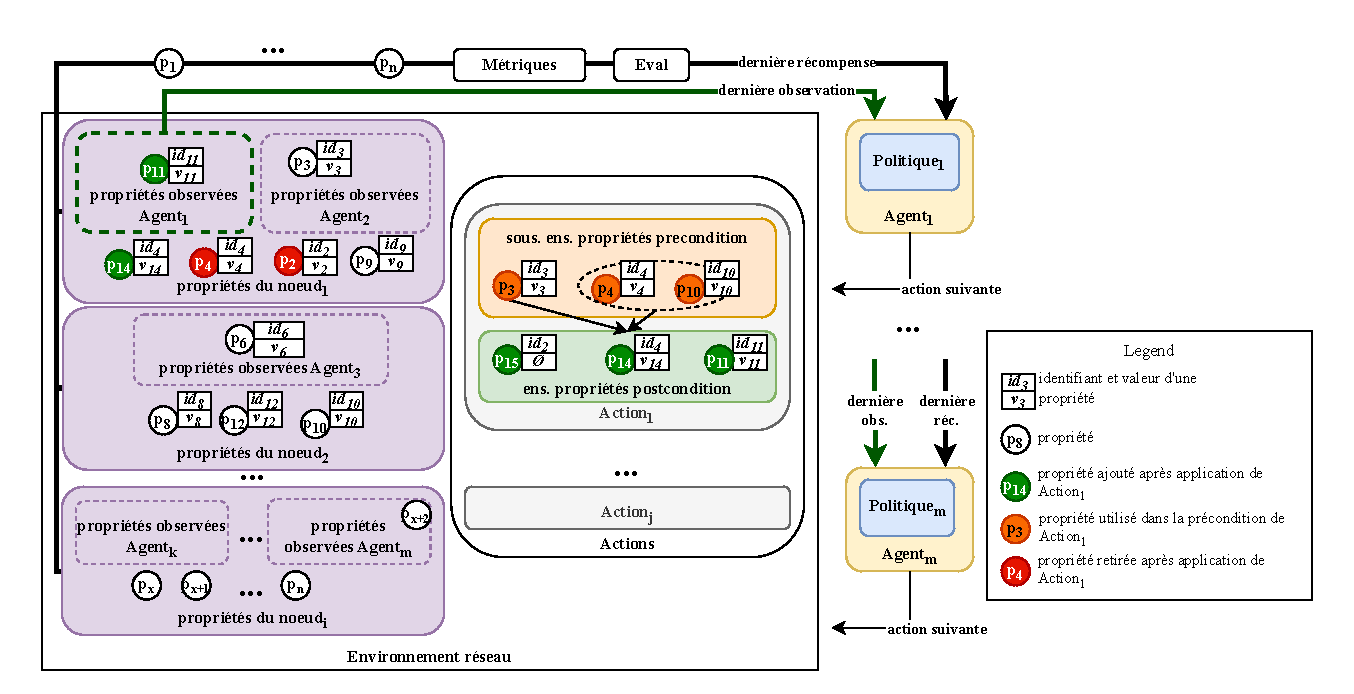
\includegraphics[width=0.97\textwidth]{figures/model_example_illustration.pdf}
    \caption{An illustrative view of the simulation model}
    \label{fig:model_example_illustration}
\end{figure*}

\noindent
From a global view the proposed Dec-POMDP model expresses an environment state as the set of nodes properties including agents observable properties. We define a property as a couple made of an identifier and a value. The environment state is changed when an action is applied by an agent. An action can be applied only if the boolean property-based pre-condition is satisfied in the current environment state. The resulting state is then modified depending on post-condition ultimately leading some new properties to be added while some others are deleted. After an action is successfully applied by an agent, observable properties of the same agent are returned to it as observations from that new state. A reward is also computed based on the current state and returned to the agent. An agent is chosen to be modeled as a behavior function which has to select the next action to be made depending on received observations and rewards.

There are different ways for several agents to be executed in a same environment tweaking with the number of agents to execute in a time step and the number of actions to be played by an agent in a time step. Even though not realistic, we chose the \textquote{Agent Environment Cycle}~\cite{jk2020} as a first approximation by having several agents playing one action in each turn in a sequential cyclic manner. The iteration cycle is presented through an illustrative informal view of the simulation model in Figure~\ref{fig:model_example_illustration}. It shows $i$ nodes with their properties including the $m$ agents' observed ones; and how each of the available $j$ actions associates a pre-condition set of properties subsets to a subset of new properties to be added in the environment optionally deleting obsolete properties having the same identifiers as the new properties' ones: \begin{enumerate*}[label=\arabic*),itemjoin={;\quad}]     
    \item An agent chooses an action from previous observations and rewards according to a behavior function. In Figure~\ref{fig:model_example_illustration}, as $Agent_1$ begins its first turn, it receives only initial observations ($p_{1}$) and zero rewards and chooses $Action_1$
    
    \item The environment is updated by a transition function depending on the current state and the action taken by the agent (change of properties once the pre-condition is satisfied). An action is used to change the environment properties by updating the relation between property identifiers and property values.
    For instance, in Figure~\ref{fig:model_example_illustration}, in current state, $Node_1$ properties are $p_1,p_3,p_4,p_2,p_9$. When $Action_1$ is applied, the relation associate subsets $\{p_3\}$ or $\{p_4, \allowbreak p_{10}\}$ to $\{p_{15}, \allowbreak p_{14}, \allowbreak p_{11}\}$. The property based pre-condition can be understood as $p_3 \lor (p_4 \land p_{10})$. As $p_{15}$ and $p_{14}$ are identified by $ID_4$ and $ID_2$ which already respectively define $p_{2}$ and $p_{4}$, $p_{4}$ and $p_{2}$ are deleted and $p_{11}$ and $p_{14}$ are added ($p_{15}$ is not added as $id_2$ is not associated with any value)
    
    \item Observed properties are returned to the current executor agent for its next turn. In Figure~\ref{fig:model_example_illustration} $p_{11}$ and $p_1$ are returned after $Action_1$ is applied.

\end{enumerate*}

\noindent
Agents are selected following a sequential order. Each one receives last observations and rewards from their last turn (or just initial observation and zero rewards if they are on their first turn); chooses the next action to play in its current turn. Once the last agent has finished playing (such as $Agent_m$), rewards are computed and sent to cyber-attackers and cyber-defenders based on the evaluation of the collected metrics from last state. Then, the agents play again following the same sequential order for another iteration.


\subsection{Formal Dec-POMDP modeling}

We set the elements related to the properties of the nodes, agents and actions of the following environment:

\begin{itemize}

    \item $Ag = \{ag_1,..,ag_{|Ag|}\}$: The set of agents (cyber-attackers and cyber-defenders).
    % \begin{itemize}
    %     \item With $Attackers \subseteq Ag$: The set of attacker agents
    %     \item With $Defenders \subseteq Ag$: The set of defender agents
    % \end{itemize}

    \item We call the couple $p = (id_{j}, v_{j})$ with $id_j \in {ID}$ and $v_j \in V$, a property.
    \begin{itemize}
        \item $ID$: The set of property identifiers optionally indicating how are organized the properties in a non-flat data structure (such as $PC1.processes.agents.agent1$). These property identifiers may be used for a file path, the type of operating system used in a node, a used command line by an agent\dots
        \item $V$: The set of property values. These may include the content of a file, a full description of the operating system, the output result of a command line\dots
        % \item $Values: ID \rightarrow \mathcal{P}(V) = \{(id_{j}, V_{j}) \: | \: id_j \in {ID},$ $V_j \in \mathcal{P}(V)\}$: a bijection associating a property identifier to the set of the different values it can be associated with. For instance, a the identifier $ls\_command\_output$ may be associated with the following values $\{file.txt,\{file.txt,passwd.txt\}\}$
    \end{itemize}

    \item $P_{j} = \{ p_1, .., p_{|P_{j}|} \}$: The set of the $p_{l}$ properties (with $l \in \{1,..,|P_{j}|\}$) of node $j$ ($j \in \mathbb{N} $). For example, such properties may include some running process IDs, files list in a folder, type of operating system with description, specific knowledge of an agent, etc.
    \begin{itemize}
        \item $P = P_1 \cup P_2 .. \cup P_{|P|} $: The set of all the node properties.
    \end{itemize}

    \item $Obs: \mathcal{P}(P) \times Ag \rightarrow \mathcal{P}(P_{Ag}), P_{Ag} \subset P$: A relation which associates node properties and an agent with the observed property subset by the agent.
    
    \item $Action: P_{pre} \rightarrow P_{post}$: A relation which associates a property subset implied by an equivalent conjunctive boolean pre-condition ($P_{pre} \subset \mathcal{P}(P)$) to a subset of all of the properties of the post-condition ($P_{post} \in \mathcal{P}(P)$). For example, the properties $p_1 = (agent\_X\_privilege\_level, \allowbreak root)$, $p_2 = (agent\_X\_accessed\_text\_editor, \allowbreak Vim)$ and $p_3 = (agent\_X\_bashrc\_known\_filepath, \allowbreak /home/user/.bashrc)$ can make a pre-condition ($p_1 \land p_2 \land p_3$) to associate a new set of property containing $p4 = (bashrc\_file\_modified\_by\_X\_agent, \top)$. Two pre-condition subsets can be associated to the same post-condition subset to model a boolean disjunction.

    \item $Metrics: \mathcal{P}(P) \times A \rightarrow \mathbb{R}^{n}$: Gives metrics associated with a set of properties and joint action. For example, the number of nodes still active, lateral moves, etc.

\end{itemize}


Using the formal description of a Dec-POMDP~\cite{OliehoekA16}, we propose the following model:

\begin{itemize}
    \item $S = \{s_1, ..s_{|S|}\}, s_{i} \subseteq P \: and \: 1 \le i \le |S|$: The space of states as possible property sets.

    \item $A_{i} = \{a_{i}^{1},..,a_{i}^{|A_{i}|}\}, a_{i}^j \in Action \: and \: 1 \le j \le |A_i|$: The set of possible actions for agent $i$.

    \item $T$ : The set of conditional transition probabilities between states
    \begin{itemize}
        \item With $T(s,a,s') = \probP(s'|s,a)$, the relation which associates probability to go to state $s' \in S$ from state $s \in S$ knowing we played $a = (P^a_{pre} \times P^a_{post}) \in A$ with $P^a_{pre} \subset \mathcal{P}(P)$ and $P^a_{post} \in \mathcal{P}(P)$
        \item With $\probP(s'|s,a) = 0$ if $s$ does not satisfy the pre-condition of $a$ (i.e $\exists \: P_{pre_s}^{a} \in P_{pre}^{a} \: | \: P_{pre_s}^{a} \not\in \mathcal{P}(s)$).
        \item With $s' = (s - \{p_l=(id_l, v_l) \: | \: p_l \in s \: and$ $id_l \in \{id_k \: | \: (id_k, v_k) \in P^a_{post} \: and \: v_k \neq \varnothing\}\}) \cup P^a_{post}$
    \end{itemize}
    
    \item $R: S \times A \rightarrow \mathbb{R}^2 = Eval \circ Metrics$: The reward function that takes a state and an action and associates a performance indicator (using the state's metrics) for attackers and defenders.
    \begin{itemize}
        \item With $Eval: \mathbb{R}^{n} \rightarrow \mathbb{R}^2$, associates a metric vector to a a reward for cyber-attackers and cyber-defenders.
    \end{itemize}
    
    \item $\Omega_{i} \subset Range(Obs \: | \: \{ (s, ag_i) | s \in S \: and \: ag_i \in Ag \}) \subset P$: The set of observable properties for agent $ag_i$. For example, the content of a file, the log output of a command, the result of a port scan, etc.
    \begin{itemize}
        \item $\Omega = \Omega_1 \cup \Omega_2 .. \cup \Omega_{|Ag|} = Range(Obs)$: The set of all the observable properties for all agent.
    \end{itemize}

    \item $O$ : The set of conditional observation probabilities.
    \begin{itemize}
        \item With $O(s',a,o) = \probP(o|s',a)$, the relation which associates the probability to observe an observation $o \subset \Omega$ from state $s' \in S$ induced by $a \in A$
        \item With $\probP(o|s',a) = 0$ if the state $s' \in S$ does not contain the properties of $o \subset \Omega$ (i.e $o \not\in \mathcal{P}(s')$). For example, an agent plays the action $x\_reads\_a\_log\_file$, a new state results from which a property belonging to the knowledge of agent x is $(log\_file\_content\_known\_by\_x, \allowbreak abc)$. This property will be therefore included in the returned observations to agent x. 
    \end{itemize}

\end{itemize}


\subsection{Attack/defense scenarios integration\label{sec:ad_integration}}

\noindent
From a raw perspective, the proposed formal Dec-POMDP modeling relies on actions to simulate how a real networked system would react including vulnerabilities and countermeasures applied by cyber-attacker and cyber-defender agents.

A first challenge is to build a representative attack/defense scenario of a networked system comprising vulnerabilities to allow rendering an attack by linking the only available pieces of information (such as known tactics, techniques and procedures from MITRE ATT\&CK) and by choosing relevant defense countermeasures (from MITRE ATT\&CK mitigations) and a deployment environment. A second challenge is to establish the actions to match the attack/defense scenario. As actions modify the environment properties, they also impact possible states space and the transitions between them.
Moreover, when considering a low abstraction level, numerous simple actions may allow describing the operated changes in the network finely. Yet, doing so increases the number of actions, and even more the number of states for they are combinations of action effects.

These challenges are directly linked to studied issues about automated generation of attack graphs using available databases optionally integrating artificial intelligence techniques as in ~\cite{GFalco2018}. We do not intend to focus more on these issues as they are out of the scope of this work.

\

\noindent
\textbf{MITRE ATT\&CK integration approach}: We suggest a high-level manual approach we used to integrate MITRE ATT\&CK information as an AD tree for it formalizes actions to be played in a scenario and their interactions with the environment. It is aimed at being helpful to establish the attack/defense actions to be finally integrated in the simulator:
\begin{enumerate*}[label=\arabic*),itemjoin={;\quad}]

    \item For a given Advanced Persistent Threat (APT), we identified relevant tactics and techniques and procedures from MITRE ATT\&CK that seemed relevant for a networked system
    
    \item We produced a description linking identified tactics together and associated techniques, sub-techniques and procedures to create a scenario that describes how the APT group could attack the networked system. This step defines the network topology with its main properties
    %(such as a company network made up of several dedicated database servers communicating through FTP and HTTP, etc.)

    \item We created an AD tree as proposed in ~\cite{BKordy2010} with tactics as top action goals while techniques, sub-techniques and procedures are in the lower part of the tree. We made sure to have several paths to reach a same top-action goal. We paid attention to define each attack action with property based pre-condition and property post-conditions in the environment

    \item We extracted the MITRE ATT\&CK techniques/sub-techniques related detection and mitigations we added in the AD tree to decorate the attack nodes. We paid attention to define each defense actions with property based pre-condition and property post-conditions in the environment.



    % \item We also listed and defined the main deployment specific environmental actions from deployment environment previous description or extended attack/defense actions which are common to both cyber-defenders and cyber-attackers. This step brings a more realistic environment providing a representative number of plausible actions an agent can choose in many systems.
    % These common actions could include at least:
    % \begin{itemize}
    %     \item Reading and writing files
    %     \item Creating, deleting, copying, moving, renaming, modifying properties of files/folders.
    %     \item Go into a folder, go to the parent folder
    %     \item Focusing a file/folder for applying future actions
    %     \item Execute binary file
    %     \item Using network protocol (such as HTTP, FTP, SSH, etc.).
    %     \item Some other interactions with basic command lines about system monitoring or controlling.
    % \end{itemize}
    % Then, associated environmental properties should describe a file system, a terminal interface, port with rules, operating system parameters properties, etc.

\end{enumerate*}

\subsection{Simulation model implementation}

\noindent
Potential works to implement our model include: NeSSi2~\cite{DGrunewald2011} which is an agent-based simulation platform aiming to model only packet-level description of a networked system and the effects of DDoS attacks; and Kotenko et al.~\cite{IKotenko2007} which relies on OMNet++~\cite{Varga2010} to model and simulate cooperative cyber-defense agents against network attacks combining discrete-event simulation, multi-agent approach and packet-level simulation of network protocols.
% Additionally, to overcome limited realism, emulators using virtual machines and integrated with offensive tools have been pushed forward, such as DCAFE~\cite{GRush2014} and SVED~\cite{HHannes2016}.
However, among these, none can fully meet both the consideration of a multi-agent cyber environment for a Dec-POMDP model.
%and the need for code accessibility (open source code).

\begin{figure}
    \centering
    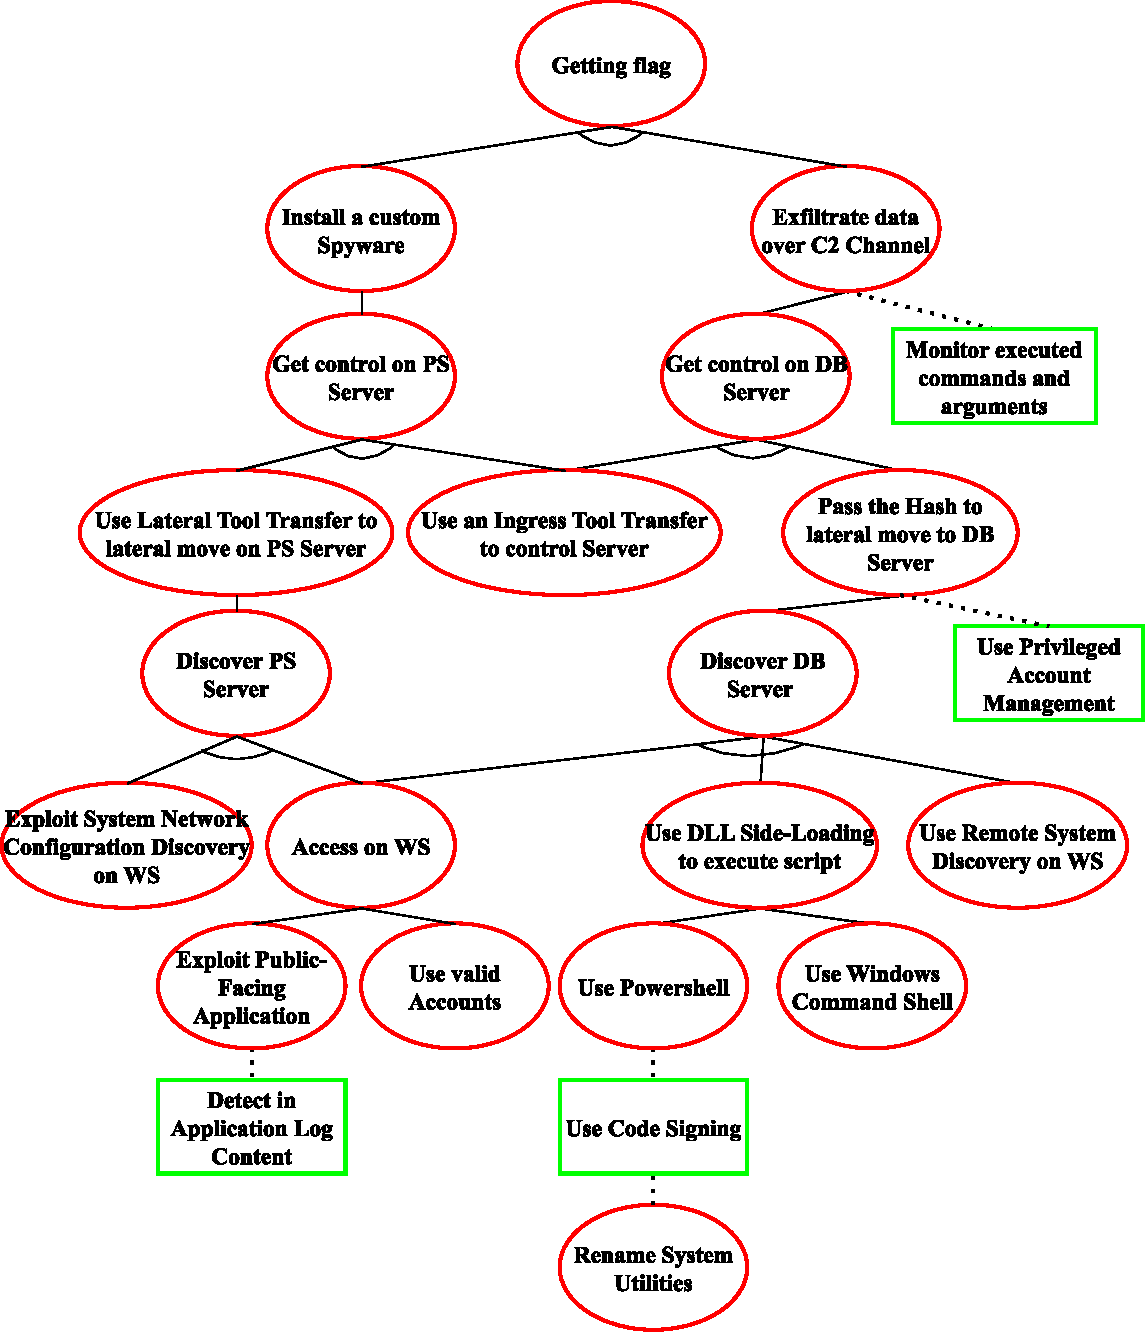
\includegraphics[width=\linewidth]{figures/ADTree.pdf}
    \caption{An overview of the proposed attack/defense AD Tree}
    \label{fig:ADTree}
\end{figure}

Yet, we identified discrete-event simulators with a single cyber-attacker such as CYST\cite{drasar_session-level_2020} or CyberBattleSim~\cite{cyberbattlesim}, which both provide a suited network simulation and evaluation approach towards an implementation of our model as their underlying models can be extended for several agents. Inspired by these approaches, we used \textit{PettingZoo}~\cite{jk2020} as a fundamental platform to implement our Dec-POMDP model onto which we aimed to implement a simulated network. \textit{PettingZoo} provides a framework where the designer has tools to facilitate the implementation of the space of observations, actions, management of agents at each turn and associated rewards.

% \begin{figure}
%      \centering
%      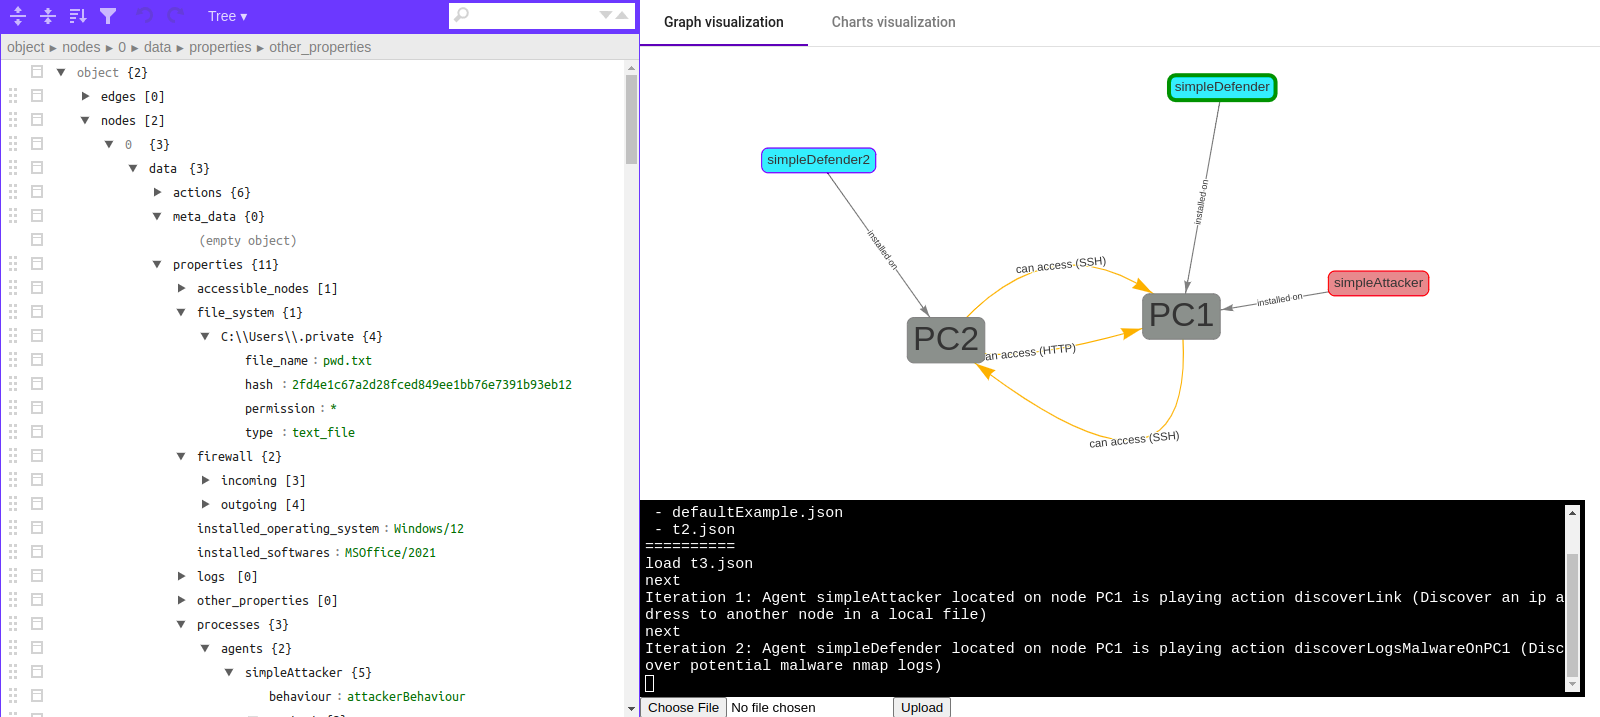
\includegraphics[width=\linewidth]{figures/interface_MCAS.png}
%      \caption{Simulator interface overview}
%      \label{fig:simulator_interface}
% \end{figure}

The development of our model has led to the \textquote{Multi Cyber Agent Simulator} (MCAS)~\cite{MCASWebsite} simulator. In the current state of development, this simulator allows loading/saving a \textit{json} file describing the nodes properties and actions of the environment and the defined agents with their behaviors; and launching the execution of the agents of this environment in turn-by-turn mode via the terminal. It is possible to view the environment properties in real time and visualize the environment in the form of a graph. Metrics are displayed as well.



\section{MITRE ATT\&CK based case study}

% \rem{Expliquer pourquoi on veut tester les capacités du simulateur -> illustration de comment fonctionne le simulateur}
% \rem{Gallium APT, pourquoi ce choix ? pourquoi ce cas d'étude inspiré de ça ? Qu'est-ce qui est interessant dans Gallium APT ? Type d'attaque/ coordination d'attaque ?}

\noindent
Intending to assess coordinated attacks and collective defense, we chose GALLIUM APT (a cyberespionage group active since 2012), for it allows defining several concurrent attacks.


\subsection{Network topology}

% \rem{Pour chaque élément présent dans la figure, faire le lien avec les éléments cités dans la présentation de la topologie...}

\noindent
Based on some GALLIUM APT tactics we selected some associated techniques/sub-techniques to propose a small company like networked environment, presented in Figure~\ref{fig:scenario_network_topology}. It is divided in 5 subnets communicating through implicit routers positioned after a firewall:
The outside subnet used to represent external attackers as if in the same network for convenience. It includes two desktop computers (At1 and At2).
The Demilitarized Zone (DMZ) subnet is used to separate devices that are accessible from the Internet from the rest of the company's network. The servers in the DMZ include a web server (WS), an email server (ES), a VPN server (VPN), and a FTP server (FTP), all connected bidirectionally both to outside and inside the company network.
The first local area network (ACC) subnet used to connect devices within the accounting department of the company where employee are working in. It contains two employee workstations (E1 and E2) and a Chief Technical Officer workstation (CTO), all connected bidirectionally to the DMZ. % and only accessible from SRV (defined below);
The second local area network (MAR) subnet used to connect devices within the marketing department of the company. It contains a printer server (PS), one employee workstations (E3) and tablet terminal (TAB) connected via a wireless access point, all connected bidirectionally to the DMZ. %and only accessible from SRV (defined below);
The third local area network (SRV) subnet used to connect the company devices providing services. It contains an API server (API), a database server (DB), and a domain controller (DC).

\begin{figure}
    \centering
    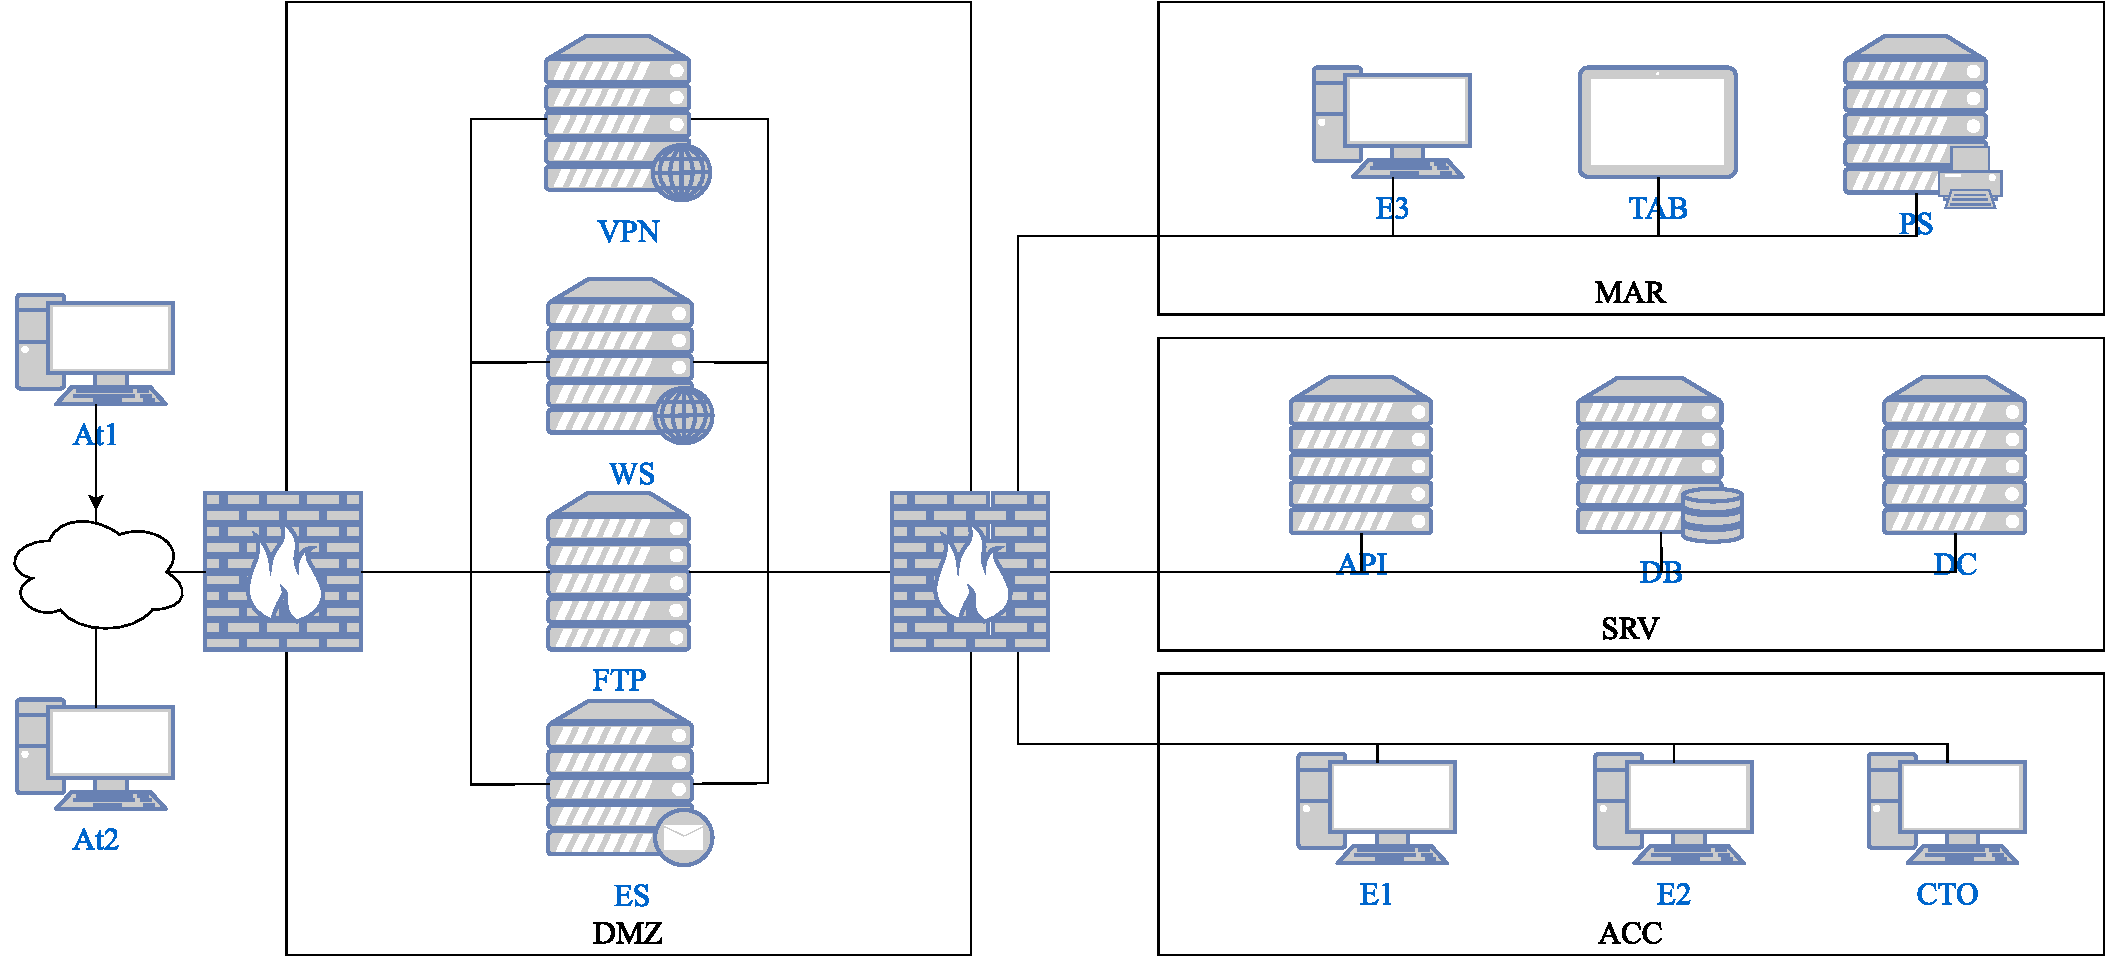
\includegraphics[width=\linewidth]{figures/topology.pdf}
    \caption{Proposed small-scale company network topology}
    \label{fig:scenario_network_topology}
\end{figure}


%These devices are accessible from the DMZ and from the CTO. API is also accessible via a VPN tunnel from the outside.

% The simulated machines are populated with files, folders, firewall rules, network services, and so on, so both attackers and defenders can have more actions to interact.


\subsection{Scenario and agent implementation with evaluation}

\begin{figure}
    \centering
    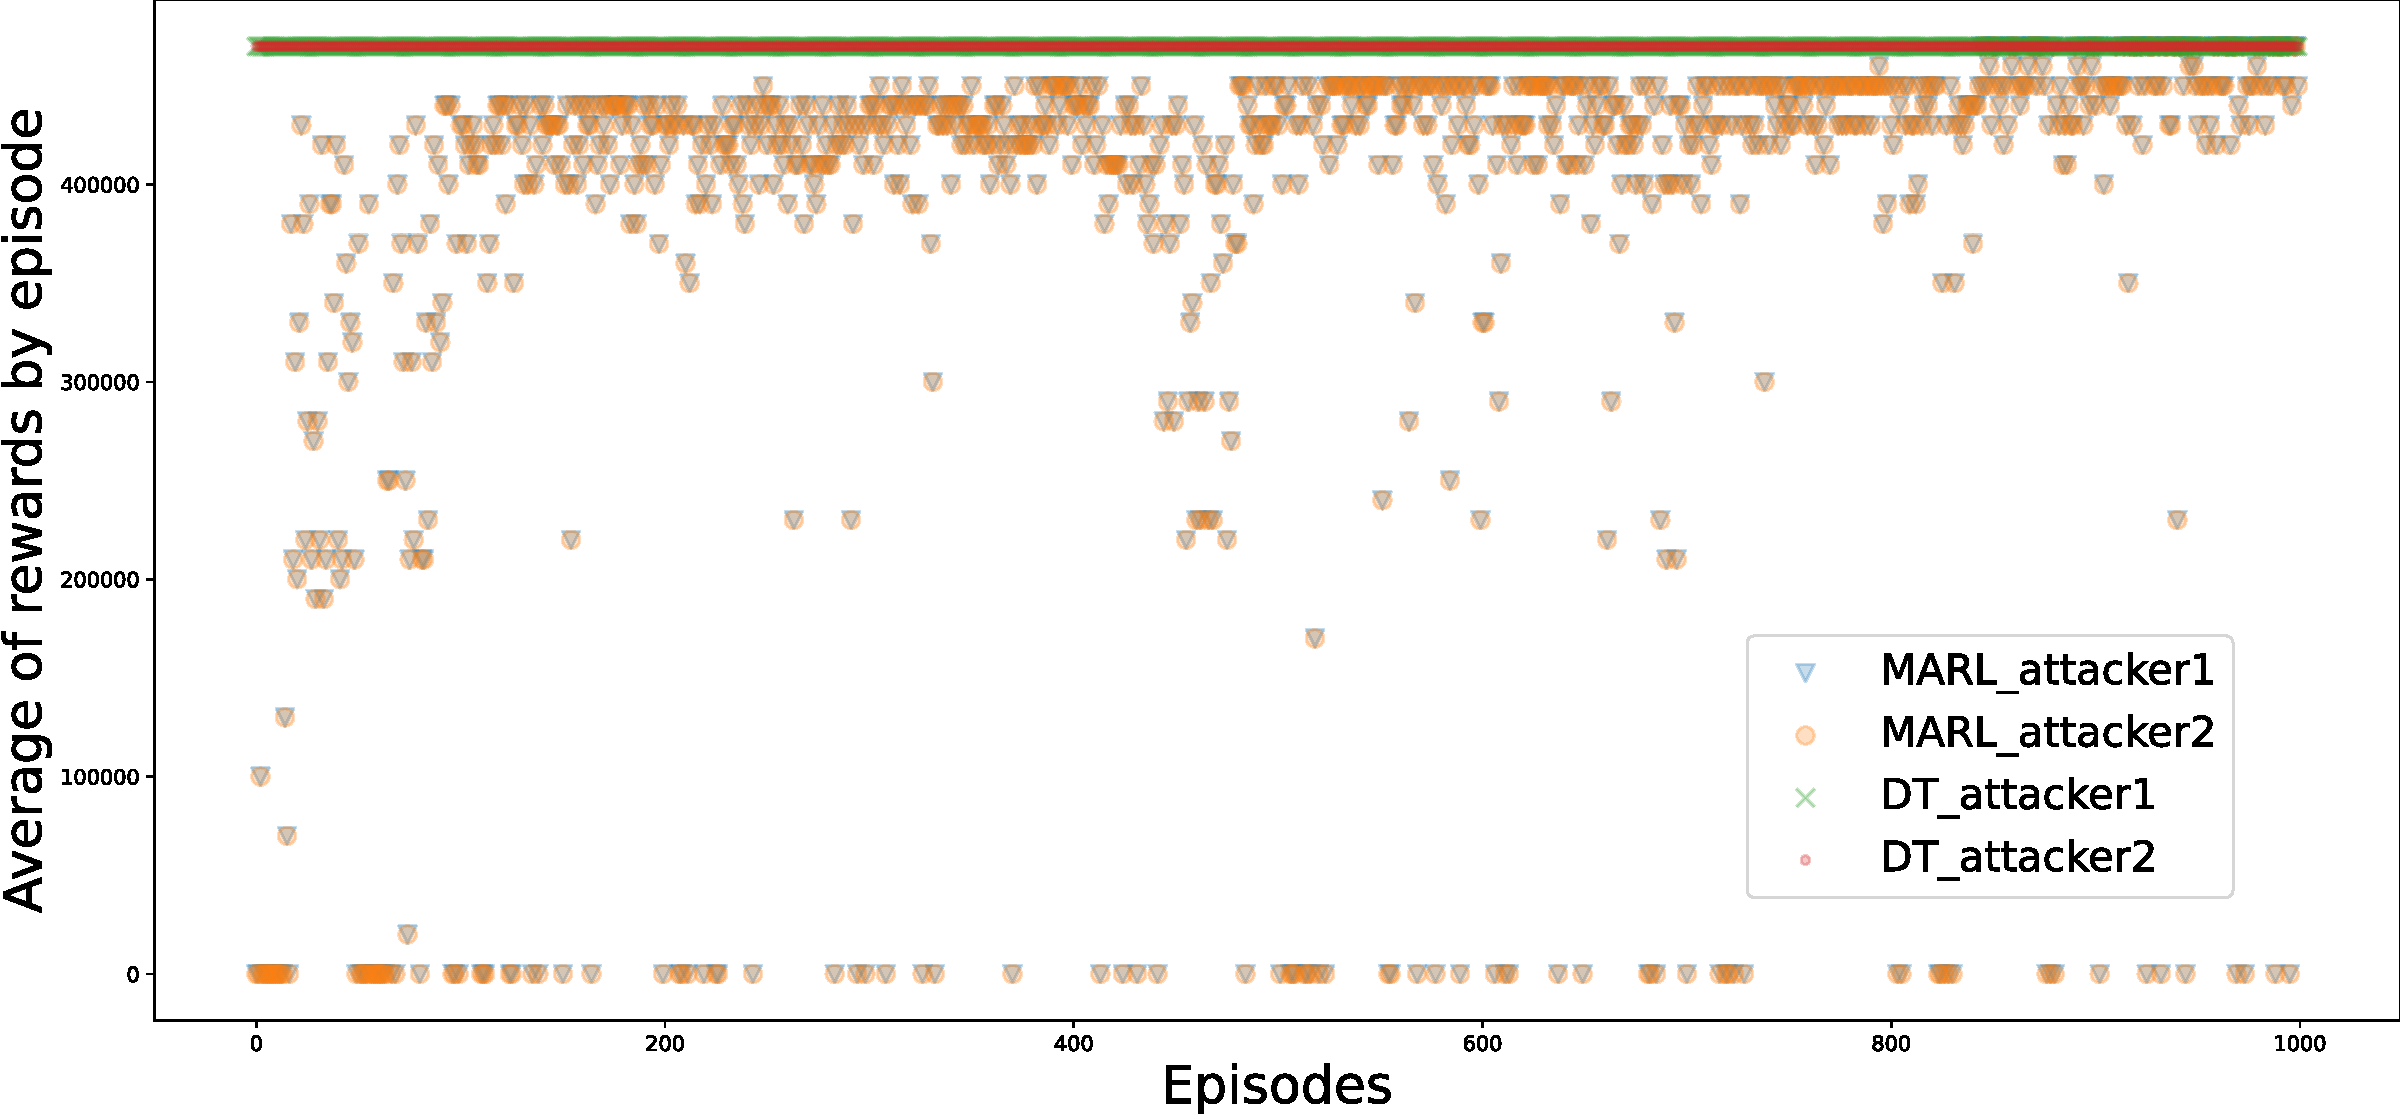
\includegraphics[width=\linewidth]{figures/graphs.pdf}
    \caption{An evolution of the rewards average according to episodes in small-scale tests with MARL and Decision Tree Approaches with inactive cyber-defense
    }
    \label{fig:graphs}
\end{figure}

\noindent
The cyber-attacker agents are initially deployed on At1 and At2 and the cyber-defender agents are deployed on WS and DB. The ultimate attackers' goals is to get data from the DB server and installing one spyware on the printer server PS. Following our approach in ~\ref{sec:ad_integration} we propose an AD tree presented in Figure~\ref{fig:ADTree}. It only shows the paths of the attacks to follow to reach the ultimate goal while the defender actions can prevent these at several stages of the attack.
We first interested in setting up the two cyber-attackers behaviors, then the two cyber-defenders' ones. We simulated an abstracted version of the scenario over 1000 episodes.

% In addition, we implemented some other common actions to interact with the file system, OS configuration, firewall configuration, and network services. These actions can be derived from the attack/defense actions but are implicitly not shown in the AD tree. Yet, they are taken into account in the simulation so agents can explore action paths even if this does not lead to an ultimate attacker goal.


%\subsection{Scenario execution and evaluation}

\noindent
\textbf{Random approach}: \quad The random agent only choose its actions by exploring the whole action space without any criteria until reaching the goal. In our case study, the shortest action path for attackers to reach the ultimate goal contains 16 different actions among the 30 defined actions, hence a low probability of $(1/30)^{16}$.
This approach allows getting a benchmark of unexpected edge failure cases and to compare with other types of agent.

\noindent
\textbf{Decision Tree (DT) approach}: \quad The decision tree was applied to get a reference when cyber-attackers or cyber-defenders already know the best action to take as the role of each agent is defined by a DT.
In Figure~\ref{fig:graphs}, the $DT\_attacker1$ follows an action path to reach the goal of installing a custom spyware in PS. In the same time, $DT\_attacker2$ reaches the goal of exfiltrating data in DB and completing the action path by getting the flag. Then we added the defenders $DT\_defender1$ which has to detect malicious logs on WS and $DT\_defender2$ which has to use privilege account management or monitor the executed commands and arguments on DB. We observed the attackers to be unable to reach the ultimate goal.

\noindent
\textbf{Multi-Agent Reinforcement Learning (MARL) approach}: \quad Q-Learning~\cite{CWatkins1992} was applied with curriculum learning for first the attackers learn how to reach the ultimate attack goal before adding defenders.
In the Figure~\ref{fig:graphs}, $MARL\_attacker1$ and $MARL\_attacker2$ follow a same behavior ultimately refining the applied actions to the relevant ones to reach the ultimate goal. After several episodes, chosen action paths by the attackers tend to be as efficient as the DT paths. When adding the defenders $MARL\_defender1$ and $MARL\_defender2$, we verified the attackers to be less and less able to reach the ultimate goal.


\section{Conclusion and perspectives}

\noindent
We proposed a Dec-POMDP modeling of networked node likely to be attacked and defended by agents. This model aims to integrate scenarios. The implementation of this model led to a simulator whose some capabilities have been assessed through a MITRE ATT\&CK scenario. Using three approaches, we briefly checked how decision tree, random and reinforcement learning approaches can be applied to agent for comparison.
Willing to take advantage of this simulation approach to address realistic issues related to cyber-defenders, particularly in the AICA context, we identified the main limitations to overcome:
automating the integration of more realistic scenarios leveraging on a basis of common actions and properties so agents can explore and act as in seemingly similar to reality information systems;
establishing a way to use the benefits of results obtained with simulations for emulated or real systems while maintaining agent behaviors during deployment;
having more coordination between agents, such as several entry points or scenarios with needed communication to reach a goal\dots;
and introducing new constraints in actions (such as cost, execution duration, etc.).


\section{Essaim de drones}

% TODO : A ajouter comme le cas d'étude "Essaim de drones"
% \usepackage{xcolor}
% \usepackage[hang, flushmargin]{footmisc}
% \usepackage[
% colorlinks=false, % don't highlight links in color
% linkbordercolor=green, % set border color for internal links
% citebordercolor=green, % set border color for citations
% filebordercolor=magenta, % set border color for file links
% urlbordercolor=cyan, % set border color for URLs
% pdfborder={0 0 1}, % determine border around links
% linkcolor=black,
% citecolor=black,
% filecolor=black,
% urlcolor=black,
% ]{hyperref}
% \usepackage{footnotebackref}

% \usepackage{cite}
% \usepackage{amsmath,amssymb,amsfonts}
% \usepackage{algorithmic}
% \usepackage{graphicx}
% \usepackage{textcomp}

% \def\BibTeX{{\rm B\kern-.05em{\sc i\kern-.025em b}\kern-.08em
%     T\kern-.1667em\lower.7ex\hbox{E}\kern-.125emX}}

% \usepackage[english]{babel}
% \addto\extrasenglish{  
%     \def\figureautorefname{Figure}
%     \def\tableautorefname{Table}
%     \def\algorithmautorefname{Algorithm}
%     \def\sectionautorefname{Section}
%     \def\subsectionautorefname{Subsection}
% }

% \newcommand{\supertiny}{\fontsize{1}{2}\selectfont}

% \usepackage{catoptions}
% \makeatletter

% \def\Autoref#1{%
%   \begingroup
%   \edef\reserved@a{\cpttrimspaces{#1}}%
%   \ifcsndefTF{r@#1}{%
%     \xaftercsname{\expandafter\testreftype\@fourthoffive}
%       {r@\reserved@a}.\\{#1}%
%   }{%
%     \ref{#1}%
%   }%
%   \endgroup
% }
% \def\testreftype#1.#2\\#3{%
%   \ifcsndefTF{#1autorefname}{%
%     \def\reserved@a##1##2\@nil{%
%       \uppercase{\def\ref@name{##1}}%
%       \csn@edef{#1autorefname}{\ref@name##2}%
%       \autoref{#3}%
%     }%
%     \reserved@a#1\@nil
%   }{%
%     \autoref{#3}%
%   }%
% }
% \makeatother

% \usepackage[T1]{fontenc}
% \usepackage{graphicx}
% %\usepackage{color}
% %\renewcommand\UrlFont{\color{blue}\rmfamily}

% \usepackage{amsmath,amssymb,amsfonts}
% \usepackage[inline, shortlabels]{enumitem}
% \usepackage{tabularx}
% \usepackage{caption}
% \usepackage{listings}
% % \usepackage{titlesec}
% \usepackage{ragged2e}

% \usepackage{xurl}
% % \usepackage[hyphens]{url}
% \usepackage{pifont}
% \usepackage{multirow}
% \usepackage[linesnumbered,ruled,vlined]{algorithm2e}
% \usepackage{float}
% \usepackage{listings}
% \usepackage{xcolor}

% \definecolor{codegreen}{rgb}{0,0.6,0}
% \definecolor{codegray}{rgb}{0.5,0.5,0.5}
% \definecolor{codepurple}{rgb}{0.58,0,0.82}
% \definecolor{backcolour}{rgb}{0.95,0.95,0.92}

% \lstdefinestyle{mystyle}{
%     backgroundcolor=\color{backcolour},   
%     commentstyle=\color{codegreen},
%     keywordstyle=\color{magenta},
%     numberstyle=\tiny\color{codegray},
%     stringstyle=\color{codepurple},
%     basicstyle=\footnotesize,
%     breakatwhitespace=false,         
%     breaklines=true,                 
%     captionpos=b,                    
%     keepspaces=true,                 
%     numbers=left,                    
%     numbersep=5pt,                  
%     showspaces=false,                
%     showstringspaces=false,
%     showtabs=false,                  
%     tabsize=2
% }

% \lstset{style=mystyle}

% % --- Tickz
% \usepackage{physics}
% \usepackage{amsmath}
% \usepackage{tikz}
% \usepackage{mathdots}
% \usepackage{yhmath}
% \usepackage{cancel}
% \usepackage{color}
% \usepackage{siunitx}
% \usepackage{array}
% \usepackage{multirow}
% \usepackage{amssymb}
% \usepackage{gensymb}
% \usepackage{tabularx}
% \usepackage{extarrows}
% \usepackage{booktabs}
% \usetikzlibrary{fadings}
% \usetikzlibrary{patterns}
% \usetikzlibrary{shadows.blur}
% \usetikzlibrary{shapes}

% % ---------
% % \usepackage{titlesec}
% \usepackage{pdfpages}
% \usepackage{booktabs}
% \usepackage{csquotes}
% \usepackage{lipsum}  
% \usepackage{arydshln}
% \usepackage{smartdiagram}
% \usepackage{textcomp}
% \usepackage{tabularray}\UseTblrLibrary{varwidth}
% \usepackage{xcolor}
% \def\BibTeX{{\rm B\kern-.05em{\sc i\kern-.025em b}\kern-.08em
%     T\kern-.1667em\lower.7ex\hbox{E}\kern-.125emX}}
% \usepackage{cite}
% \usepackage{amsmath}
% \newcommand{\probP}{\text{I\kern-0.15em P}}
% \usepackage{etoolbox}
% \patchcmd{\thebibliography}{\section*{\refname}}{}{}{}

% \setlength\tabcolsep{0.5pt}

% \newcommand{\before}[1]{\textcolor{red}{#1}}
% \newcommand{\after}[1]{\textcolor{green}{#1}}

% \newcommand{\old}[1]{\textcolor{orange}{#1}}
% \newcommand{\rem}[1]{\textcolor{red}{#1}}
% \newcommand{\todo}[1]{\textcolor{orange}{\newline \textit{\textbf{TODO:} #1}} \newline \newline }



% \newcounter{relation}
% \setcounter{relation}{0}
% \renewcommand{\therelation}{\arabic{relation}}
% \newcommand{\relationautorefname}{Relation}

% \newenvironment{relation}[1][]{%
%     \refstepcounter{relation}%
%     \noindent \raggedright \textit{\textbf{Relation. \therelation}} \hfill$}
% {%
% $ \hfill \phantom{x}

% }

% ====================================================

\section{Introduction}
\label{sec:introduction}

\textit{Les agents autonomes intelligents de cyberdéfense}~\cite{Kott2023} (AICA) sont des agents destinés à être déployés dans des environnements réseau afin de détecter, d'identifier et de caractériser les anomalies/attaques, de développer des contre-mesures et de les exécuter
%
\footnote{
    Théorisés par le \textit{Groupe de travail international AICA} (cf. \url{https://www.aica-iwg.org/}) et basés sur les résultats du \textit{Groupe de travail de recherche IST-152} de l'OTAN.
}.
Les recherches connexes de l'AICA soulignent le besoin croissant d'une \textit{cyberdéfense autonome} pour protéger les environnements décentralisés où les approches centralisées traditionnelles sont inefficaces, comme dans les systèmes basés sur l'IoT. Un système multi-agents (MAS) offre des mécanismes de défense robustes et adaptatifs en décomposant la complexité de la cyberdéfense en sous-tâches déléguées à des agents collaboratifs déployés dans tout le système.

L'approche descendante consiste à concevoir des MAS de cyberdéfense à partir d'architectures et de fonctionnalités prédéfinies. L'\textit{architecture de référence MAS centrée sur l'AICA} (MASCARA)~\cite{Kott2023} décrit un MAS de type AICA avec des composants qui permettent des mécanismes collaboratifs basés sur des plans ou des processus explicitement définis. Cependant, cette approche peut être coûteuse car elle nécessite une connaissance approfondie de l'environnement de déploiement, qui doit être régulièrement mise à jour en raison de changements fréquents, tels que des modifications de topologie ou de nouvelles vulnérabilités.

L'approche ascendante peut inclure l'apprentissage par renforcement multi-agents (MARL)~\cite{Albrecht2024}, où les agents apprennent à atteindre les objectifs de cyberdéfense de manière autonome, renforçant ainsi l'autonomie du MAS~\cite{hammar_stadle4_noms_23}. Malgré des résultats de simulation prometteurs, cette approche ne offre pas les garanties de sécurité nécessaires pour des applications dans le monde réel et ne fournit pas de moyens explicites pour justifier le succès ou l'échec des MAS~\cite{dulacarnold2019}. Ces problèmes entravent le développement de MAS de cyberdéfense entièrement ou semi-autonomes, tels que l'AICA, dans des environnements critiques, où les actions doivent être justifiées compte tenu de leurs conséquences potentiellement irréversibles.

Pour répondre à cette préoccupation, nous proposons de combiner ces deux points de vue en étendant la \textit{relation partielle entre l'historique des agents et le modèle organisationnel}~\cite{soule2024} (PRAHOM). PRAHOM est une approche générale qui permet d'intégrer le modèle organisationnel $\mathcal{M}OISE^+$ dans le cadre MARL, jetant ainsi les bases pour contraindre l'apprentissage. Cependant, cette perspective reste limitée dans sa mise en œuvre et se heurte à des problèmes d'évolutivité avec le nombre de spécifications organisationnelles, ce qui limite son application dans des environnements réseau complexes.

La principale contribution de cet article est le \textit{PRAHOM orienté cyberdéfense} (CoPRAHOM), inspiré du PRAHOM et des travaux connexes. Cet algorithme est spécifiquement destiné à traiter les scénarios de cyberdéfense s'appuyant sur des architectures générales de cyberdéfense telles que MASCARA. Cet algorithme permet aux utilisateurs de contraindre les agents à des rôles et des missions de cyberdéfense. Nous avons mis en œuvre des moyens pratiques pour appliquer CoPRAHOM, également dans le but de répondre aux préoccupations en matière d'évolutivité. L'un des principaux intérêts est d'assurer des garanties de sécurité en intégrant des connaissances spécifiques au domaine, telles que des règles, ou en accélérant ou stabilisant la formation en limitant l'espace de recherche.

Nous avons évalué CoPRAHOM dans le scénario simulé fourni par le 3e défi CAGE~\cite{cage_challenge_3_announcement}. Il s'agit de créer un MAS de cyberdéfense pour détecter, atténuer et éliminer les programmes malveillants dans un essaim de drones. À l'aide de CoPRAHOM, nous avons développé plusieurs modèles de MAS de cyberdéfense. Ces modèles sont utilisés par CoPRAHOM pour guider et contraindre l'entraînement des agents afin de mieux atteindre les objectifs du scénario et de garantir les exigences de sécurité. Nous vérifions que les agents entraînés présentent les stratégies collectives attendues tout en étant affinés tout au long de l'entraînement, ce qui rend le score global comparable à celui des meilleures entrées du classement.

Le reste de cet article est organisé comme suit. \autoref{sec:marl_background} présente les principes fondamentaux du MARL. \autoref{sec:related_works} passe en revue les travaux connexes sur le MARL pour la cyberdéfense et la surveillance de la formation des agents. \autoref{sec:marl_moise_linking} décrit le modèle $\mathcal{M}OISE^+$ et son intégration avec le MARL. \autoref{sec:coprahom} récapitule l'architecture MASCARA que nous avons utilisée conjointement avec l'algorithme CoPRAHOM et discute de sa mise en œuvre. \autoref{sec:experimental_setup} couvre la configuration expérimentale du 3e défi CAGE ainsi que les mesures et critères d'évaluation de CoPRAHOM. \autoref{sec:results_and_discussion} présente et discute les résultats bruts. Enfin, \autoref{sec:conclusion} conclut l'article et présente les orientations futures de la recherche.


\section{Contexte MARL}\label{sec:marl_background}

L'apprentissage par renforcement multi-agents (MARL) étend les principes de l'apprentissage par renforcement (RL) à des scénarios impliquant plusieurs agents en interaction. Les agents visent à maximiser la récompense cumulative globale par l'apprentissage, mais la présence d'autres agents introduit une complexité supplémentaire en raison de la nature dynamique de l'environnement.

Le MARL est souvent modélisé à l'aide du processus de décision markovien décentralisé partiellement observable (Dec-POMDP)~\cite{Beynier2013}, un cadre adapté aux environnements où les agents ont des observations limitées et différentes. Un Dec-POMDP est formellement défini comme un tuple $(S, \{A_i\}, T, R, \{\Omega_i\}, O, \gamma)$ :

\begin{itemize}
    \item $S$ : ensemble fini d'états décrivant l'environnement.
    \item $\{A_i\}$ : un ensemble d'ensembles d'actions, un pour chaque agent $i$.
    \item $T$ : La fonction de probabilité de transition d'état $T(s, \vec{a}, s') = P(s'|s, \vec{a})$, où $\vec{a}$ est l'action conjointe de tous les agents.
    \item $R$ : la fonction de récompense $R(s, \vec{a}, s')$, qui associe les états et les actions à une récompense.
    \item $\{\Omega_i\}$ : ensemble d'ensembles d'observations, un pour chaque agent $i$.
    \item $O$ : La fonction de probabilité d'observation $O(\vec{o} | s', \vec{a})$, où $\vec{o}$ est l'observation conjointe de tous les agents.
    \item $\gamma \in [0,1]$ : Le facteur d'actualisation pour les récompenses futures.
\end{itemize}

Dans MARL, chaque agent $i$ maintient une politique $\pi_i: H \times \Omega \rightarrow A$, qui mappe une action $a \in A$ à partir d'une observation $\omega \in \Omega$ et, éventuellement, de l'historique de l'agent $h \in H, h=\langle(\omega_0,a_0),(\omega_1,a_1)\dots(\omega_{n_e},a_{n_e})\rangle$ (avec $n_e \in \mathbb{N}$, le nombre d'étapes par épisode). Une politique conjointe $\pi_{\text{joint}} = (\pi_1, \pi_2, \ldots, \pi_n)$ décrit le comportement collectif de tous les agents.

L'objectif final est de trouver une politique conjointe $\pi_{\text{joint}}$ qui maximise la récompense cumulative attendue $U(\pi^*_{\text{joint}}) = \mathbb{E}\left[\sum_{t=0}^{\infty} \gamma^t R(s_t, \vec{a}_t)\right]$. Au lieu de viser uniquement un optimum global, notre approche met l'accent sur l'obtention de solutions approximatives avec une récompense suffisante.

Diverses méthodes ont été proposées pour relever les défis posés par les MARL.
%
\textbf{Les méthodes basées sur la valeur}, telles que QMIX~\cite{rashid2018}, estiment la fonction de valeur $Q(s,\vec{a})$, qui représente la récompense cumulative attendue pour un état donné $s$ et une action conjointe $\vec{a}$. Si ces méthodes ont donné des résultats prometteurs dans des scénarios simples, elles ont souvent du mal à exploiter efficacement la communication multi-agents pour améliorer les récompenses globales~\cite{oroojlooy2021review}.
%
\textbf{Les méthodes basées sur les politiques}, notamment l'optimisation de la politique proximale multi-agents (MAPPO)\cite{yu2022surprising} et le gradient de politique déterministe profond multi-agents (MADDPG)\cite{lowe2017multi}, paramètrent directement la politique sous la forme $\pi_\theta$ et l'optimisent, en utilisant éventuellement un entraînement centralisé avec une exécution décentralisée. Nous avons privilégié ces méthodes car elles ont démontré une efficacité significative dans divers contextes coopératifs et compétitifs à agents multiples~\cite{yu2022surprising}\cite{lowe2017multi}.
%
Enfin, les méthodes \textbf{Actor-Critic} combinent les approches basées sur la valeur et celles basées sur la politique. Par exemple, dans COMA (Counterfactual Multi-Agent Policy Gradients), l'acteur met à jour les paramètres de la politique dans la direction indiquée par le critique, qui évalue la politique actuelle. Bien que ces méthodes se soient révélées efficaces dans des configurations à agent unique, des efforts supplémentaires sont nécessaires pour les adapter pleinement à des scénarios multi-agents, en particulier pour gérer la complexité introduite par l'influence mutuelle des agents~\cite{papoudakis2021agent}.


\section{Travaux connexes}
\label{sec:related_works}

Nous définissons le MARL orienté organisation comme le vaste domaine de recherche englobant les études qui introduisent des spécifications explicites (telles que des règles, des rôles ou des protocoles) afin de guider ou de restreindre le processus de formation MARL pour répondre à des exigences. Bien que l'intégration explicite de spécifications organisationnelles dans le MARL ne soit pas largement traitée dans la littérature, plusieurs approches ont été proposées pour intégrer certaines contraintes dans les MAS afin de garantir que les agents se conforment à des exigences spécifiques.

\textbf{Apprentissage avec des contraintes organisationnelles} \quad
Dans \cite{cruz2020norms}, les auteurs présentent une méthode pour intégrer des normes dans les algorithmes d'apprentissage des agents, garantissant ainsi que leur comportement reste dans des limites acceptables. De plus, \cite{villatoro2011social} propose un mécanisme permettant aux agents d'apprendre et de s'adapter aux normes sociales dans des environnements dynamiques, soulignant l'importance de l'adaptation aux normes dans les MAS.
%
Un sous-ensemble pertinent de travaux appartient au domaine de l'apprentissage par renforcement guidé par des spécifications, qui vise à générer des politiques permettant d'accomplir des tâches spécifiques à l'aide de spécifications externes pour guider l'apprentissage dans la réalisation d'objectifs soumis à des contraintes données~\cite{Bansal2022}. Jothimurugan et al.~\cite{Jothimurugan2021} proposent l'apprentissage de spécifications logiques, exploitant la structure compositionnelle des spécifications pour générer des politiques pour des tâches complexes. Cependant, cela ne s'inscrit pas complètement dans le cadre MARL que nous avons défini, car cela nécessite l'introduction de spécifications logiques.

\textbf{MARL dans la cybersécurité et les opérations cyberautonomes} \quad
Le MARL a également été appliqué à la cybersécurité afin de développer des systèmes autonomes capables de se défendre contre les cybermenaces. Albrecht et al.~\cite{Albrecht2024} explorent l'utilisation du MARL pour former des agents dans des environnements dynamiques afin d'atteindre des objectifs de cybersécurité.
Comme indiqué précédemment dans Kott et al.~\cite{Kott2023}, certains travaux impliquant les AICA comprennent le développement de cadres de simulation pour la formation sur mesure d'agents autonomes dans un environnement décentralisé~\cite{Drasar2020}.
De même, dans \cite{Hammar2022}, les auteurs présentent un cadre utilisant des méthodes d'identification de systèmes pour intégrer des jumeaux numériques à MARL afin d'améliorer l'automatisation de la cybersécurité et l'applicabilité de MARL dans des systèmes réels.

\textbf{Approches basées sur des politiques} \quad
Certains travaux liés aux approches basées sur des politiques favorisent des moyens de faire respecter les contraintes organisationnelles en définissant des politiques explicites qui régissent le comportement des agents. Dans \cite{krupanski2015norm}, l'utilisation de politiques normatives est étudiée pour guider les interactions entre agents et les processus décisionnels. De plus, \cite{vos2020governing} explore l'utilisation de mécanismes de gouvernance pour faire respecter les politiques organisationnelles dans les systèmes décentralisés. Cependant, ces approches se heurtent à un manque de praticité dans leur utilisation et peuvent être difficiles à expliquer, car la plupart des politiques sont opaques et ne peuvent pas être facilement modifiées.

\textbf{Cadres intégrant les aspects organisationnels} \quad
Wang et al.~\cite{Wang2020} introduisent une approche dans laquelle des rôles émergents similaires sont encouragés à se spécialiser conjointement dans des tâches spécifiques. Tosic et al.~\cite{Tosic2010} proposent un cadre de coordination basé sur les capacités de communication des systèmes multi-agents. Zheng et al.~\cite{Zheng2018} présentent une plateforme pour le MARL qui vise à faciliter la recherche sur l'intelligence collective artificielle en fournissant un ensemble complet de mesures d'évaluation permettant de comparer les performances des algorithmes MARL. Cependant, elle ne tient pas compte des spécifications susceptibles d'inciter les agents à adhérer à un comportement attendu, tel que des missions.


Malgré ces avancées, les recherches utilisant explicitement des spécifications organisationnelles pour contraindre l'apprentissage des agents en fonction des exigences sont encore rares. À notre connaissance, aucun travail existant ne facilite la génération d'un MAS qui satisfait explicitement des contraintes organisationnelles supplémentaires. L'originalité de CoPRAHOM réside dans l'utilisation explicite d'un modèle organisationnel comme moyen général de contraindre l'apprentissage en fonction de ces exigences.

\section{Combinaison du modèle $\mathcal{M}OISE^+$ et du MARL}
\label{sec:marl_moise_linking}

Cette section présente brièvement les principes que nous proposons pour adapter MARL aux spécifications organisationnelles afin d'aligner les politiques sur les comportements attendus et les objectifs de la mission.

Le modèle $\mathcal{M}OISE^+$ fournit un cadre structuré pour définir les rôles et les interactions au sein d'un système multi-agents (MAS). Il est compatible avec MARL, ce qui permet de décrire formellement les politiques des agents. L'approche CoPRAHOM intègre les spécifications $\mathcal{M}OISE^+$ dans la formation MARL, permettant ainsi aux agents de respecter les rôles et les missions prédéfinis. $\mathcal{M}OISE^+$ définit les \textbf{spécifications organisationnelles (OS)} comme $\mathcal{OS} = \langle \mathcal{SS}, \mathcal{FS}, \mathcal{DS} \rangle$, où $\mathcal{SS}$ sont les \textbf{spécifications structurelles}, $\mathcal{FS}$ sont les \textbf{spécifications fonctionnelles} et $\mathcal{DS}$ sont les \textbf{spécifications déontiques}.

\subsection{Spécifications structurelles}

\textbf{Spécifications structurelles} ($\mathcal{SS} = \langle \mathcal{R}, \mathcal{IR}, \mathcal{G} \rangle$) décrivent la structure organisationnelle :
\begin{itemize}
    \item $\mathcal{R}_{ss}$ : tous les rôles ($\rho \in \mathcal{R}$).
    \item $\mathcal{IR}$ : relation d'héritage des rôles ($\rho_1 \sqsubset \rho_2$).
    \item $\mathcal{RG} \subseteq \mathcal{GR}$ : groupes racines, $\mathcal{GR} = \langle \mathcal{R}, \mathcal{SG}, \mathcal{L}^{intra}, \mathcal{L}^{inter}, \mathcal{C}^{intra}, \mathcal{C}^{inter}, np, ng \rangle$, où :
          \begin{itemize}
              \item $\mathcal{R}$ : Rôles non abstraits.
              \item $\mathcal{SG}$ : sous-groupes.
              \item $\mathcal{L}^{intra}$ et $\mathcal{L}^{inter}$ : Liens intra et inter groupes désignés par un triplet $(\rho_s, \rho_d, t)$, où $t \in \{acq, com, aut\}$.
              \item $\mathcal{C}^{intra}$ et $\mathcal{C}^{inter}$ : Compatibilités intra et intergroupes notées $\rho_a \bowtie \rho_b$.
              \item $np$ : cardinalité des agents dans un rôle.
              \item $ng$ : cardinalité de chaque sous-groupe.
          \end{itemize}
\end{itemize}

Les contraintes directes sur les politiques sont impraticables en raison des modèles de type boîte noire tels que les réseaux neuronaux. À la place, nous représentons les rôles sous forme de sous-ensembles historiques $\mathcal{P}(H)$ que les agents doivent générer, caractérisant les comportements attendus. Chaque rôle est mappé à un sous-ensemble historique via $rh: \mathcal{R} \rightarrow \mathcal{P}(H)$. Les politiques des agents doivent générer des historiques appartenant à ces sous-ensembles.

Nous traitons les observations complexes et volumineuses en utilisant des étiquettes pour les représenter. Le mappage $ol: \mathcal{P}(\Omega) \rightarrow \mathcal{P}(L)$ traduit les observations en étiquettes, éventuellement à l'aide d'un modèle linguistique à grande échelle (LLM) entraîné. Cela simplifie la définition des sous-ensembles d'historiques, qui peuvent être représentés par des modèles, des règles ou des scripts personnalisés.

\begin{figure}[h!]
    \centering
    


\tikzset{every picture/.style={line width=0.75pt}} %set default line width to 0.75pt        

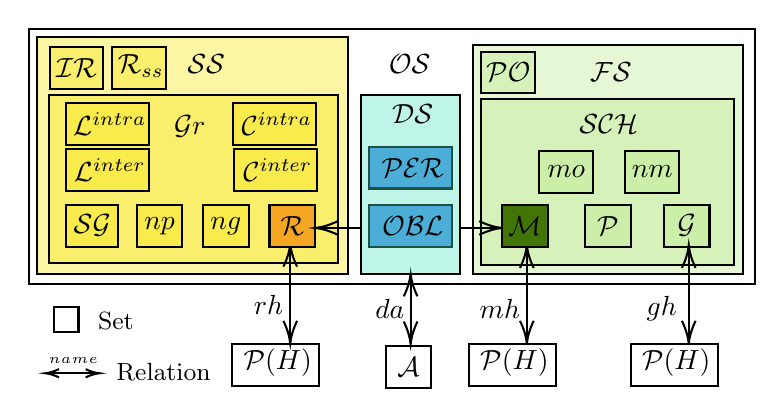
\begin{tikzpicture}[x=0.75pt,y=0.75pt,yscale=-1,xscale=1]
%uncomment if require: \path (0,1800); %set diagram left start at 0, and has height of 1800

%Shape: Rectangle [id:dp9341453924522656] 
\draw  [fill={rgb, 255:red, 255; green, 255; blue, 255 }  ,fill opacity=1 ] (160,44) -- (510,44) -- (510,167) -- (160,167) -- cycle ;
%Shape: Rectangle [id:dp4628140741854456] 
\draw  [fill={rgb, 255:red, 184; green, 233; blue, 134 }  ,fill opacity=0.34 ] (374,52) -- (504,52) -- (504,162) -- (374,162) -- cycle ;
%Shape: Rectangle [id:dp6461749357206974] 
\draw  [fill={rgb, 255:red, 184; green, 233; blue, 134 }  ,fill opacity=0.34 ] (378,78) -- (500,78) -- (500,158) -- (378,158) -- cycle ;
%Shape: Rectangle [id:dp47018118728898073] 
\draw  [fill={rgb, 255:red, 248; green, 231; blue, 28 }  ,fill opacity=0.4 ] (164,48) -- (314,48) -- (314,162) -- (164,162) -- cycle ;
%Straight Lines [id:da37904402438854] 
\draw    (400,150.31) -- (400,193.69) ;
\draw [shift={(400,195.69)}, rotate = 270] [color={rgb, 255:red, 0; green, 0; blue, 0 }  ][line width=0.75]    (10.93,-3.29) .. controls (6.95,-1.4) and (3.31,-0.3) .. (0,0) .. controls (3.31,0.3) and (6.95,1.4) .. (10.93,3.29)   ;
\draw [shift={(400,148.31)}, rotate = 90] [color={rgb, 255:red, 0; green, 0; blue, 0 }  ][line width=0.75]    (10.93,-3.29) .. controls (6.95,-1.4) and (3.31,-0.3) .. (0,0) .. controls (3.31,0.3) and (6.95,1.4) .. (10.93,3.29)   ;
%Straight Lines [id:da30557994145553513] 
\draw    (368,140) -- (386,140) ;
\draw [shift={(388,140)}, rotate = 180] [color={rgb, 255:red, 0; green, 0; blue, 0 }  ][line width=0.75]    (10.93,-3.29) .. controls (6.95,-1.4) and (3.31,-0.3) .. (0,0) .. controls (3.31,0.3) and (6.95,1.4) .. (10.93,3.29)   ;
%Shape: Rectangle [id:dp15689957472567295] 
\draw  [fill={rgb, 255:red, 248; green, 231; blue, 28 }  ,fill opacity=0.4 ] (169.56,76) -- (309.06,76) -- (309.06,157) -- (169.56,157) -- cycle ;
%Shape: Rectangle [id:dp6202366628126772] 
\draw  [fill={rgb, 255:red, 255; green, 255; blue, 255 }  ,fill opacity=1 ] (372,196) -- (414,196) -- (414,216) -- (372,216) -- cycle ;

%Shape: Rectangle [id:dp20067598884831228] 
\draw  [fill={rgb, 255:red, 248; green, 231; blue, 28 }  ,fill opacity=0.4 ] (212.06,129) -- (234.06,129) -- (234.06,149) -- (212.06,149) -- cycle ;

%Shape: Rectangle [id:dp5970765798398485] 
\draw  [fill={rgb, 255:red, 248; green, 231; blue, 28 }  ,fill opacity=0.4 ] (178.06,129) -- (203.06,129) -- (203.06,149) -- (178.06,149) -- cycle ;
%Shape: Rectangle [id:dp92237875722883] 
\draw  [fill={rgb, 255:red, 248; green, 231; blue, 28 }  ,fill opacity=0.4 ] (178.06,102) -- (218.06,102) -- (218.06,122) -- (178.06,122) -- cycle ;

%Shape: Rectangle [id:dp6591761395302378] 
\draw  [fill={rgb, 255:red, 248; green, 231; blue, 28 }  ,fill opacity=0.4 ] (178.06,80) -- (218.06,80) -- (218.06,100) -- (178.06,100) -- cycle ;

%Shape: Rectangle [id:dp11794703752595392] 
\draw  [fill={rgb, 255:red, 248; green, 231; blue, 28 }  ,fill opacity=0.4 ] (258.5,80) -- (298.5,80) -- (298.5,100) -- (258.5,100) -- cycle ;

%Shape: Rectangle [id:dp6557958558103134] 
\draw  [fill={rgb, 255:red, 248; green, 231; blue, 28 }  ,fill opacity=0.4 ] (259,102) -- (299,102) -- (299,122) -- (259,122) -- cycle ;

%Shape: Rectangle [id:dp8284992701408749] 
\draw  [fill={rgb, 255:red, 65; green, 117; blue, 5 }  ,fill opacity=1 ] (388,129) -- (410,129) -- (410,149) -- (388,149) -- cycle ;

%Shape: Rectangle [id:dp7066110016250453] 
\draw  [fill={rgb, 255:red, 248; green, 231; blue, 28 }  ,fill opacity=0.4 ] (244,129) -- (266,129) -- (266,149) -- (244,149) -- cycle ;

%Shape: Rectangle [id:dp4021333114319714] 
\draw  [fill={rgb, 255:red, 248; green, 231; blue, 28 }  ,fill opacity=0.4 ] (170.31,53) -- (195.69,53) -- (195.69,73) -- (170.31,73) -- cycle ;

%Shape: Rectangle [id:dp8476756388266236] 
\draw  [fill={rgb, 255:red, 248; green, 231; blue, 28 }  ,fill opacity=0.4 ] (200,53) -- (226,53) -- (226,73) -- (200,73) -- cycle ;

%Shape: Rectangle [id:dp07470576340681823] 
\draw  [fill={rgb, 255:red, 74; green, 144; blue, 226 }  ,fill opacity=1 ] (324,101) -- (364,101) -- (364,121) -- (324,121) -- cycle ;

%Shape: Rectangle [id:dp31407652093057714] 
\draw  [fill={rgb, 255:red, 74; green, 144; blue, 226 }  ,fill opacity=1 ] (324,129) -- (364,129) -- (364,149) -- (324,149) -- cycle ;

%Shape: Rectangle [id:dp053729126169398844] 
\draw  [fill={rgb, 255:red, 184; green, 233; blue, 134 }  ,fill opacity=0.34 ] (378,55) -- (404,55) -- (404,75) -- (378,75) -- cycle ;

%Shape: Rectangle [id:dp7720103442630182] 
\draw  [fill={rgb, 255:red, 184; green, 233; blue, 134 }  ,fill opacity=0.34 ] (405.94,103) -- (431.94,103) -- (431.94,123) -- (405.94,123) -- cycle ;

%Shape: Rectangle [id:dp3183552657000306] 
\draw  [fill={rgb, 255:red, 184; green, 233; blue, 134 }  ,fill opacity=0.34 ] (447.44,103) -- (473.44,103) -- (473.44,123) -- (447.44,123) -- cycle ;

%Shape: Rectangle [id:dp10802424702469593] 
\draw  [fill={rgb, 255:red, 184; green, 233; blue, 134 }  ,fill opacity=0.34 ] (466,129) -- (488,129) -- (488,149) -- (466,149) -- cycle ;

%Shape: Rectangle [id:dp16589412198505937] 
\draw  [fill={rgb, 255:red, 184; green, 233; blue, 134 }  ,fill opacity=0.34 ] (428,129) -- (450,129) -- (450,149) -- (428,149) -- cycle ;

%Shape: Rectangle [id:dp1270989692188249] 
\draw  [fill={rgb, 255:red, 255; green, 255; blue, 255 }  ,fill opacity=1 ] (258,196) -- (300,196) -- (300,216) -- (258,216) -- cycle ;

%Straight Lines [id:da40017392935840324] 
\draw    (286,149.69) -- (286,193.69) ;
\draw [shift={(286,195.69)}, rotate = 270] [color={rgb, 255:red, 0; green, 0; blue, 0 }  ][line width=0.75]    (10.93,-3.29) .. controls (6.95,-1.4) and (3.31,-0.3) .. (0,0) .. controls (3.31,0.3) and (6.95,1.4) .. (10.93,3.29)   ;
\draw [shift={(286,147.69)}, rotate = 90] [color={rgb, 255:red, 0; green, 0; blue, 0 }  ][line width=0.75]    (10.93,-3.29) .. controls (6.95,-1.4) and (3.31,-0.3) .. (0,0) .. controls (3.31,0.3) and (6.95,1.4) .. (10.93,3.29)   ;
%Shape: Rectangle [id:dp21027747628033966] 
\draw  [fill={rgb, 255:red, 245; green, 166; blue, 35 }  ,fill opacity=1 ] (276,129) -- (298,129) -- (298,149) -- (276,149) -- cycle ;

%Shape: Rectangle [id:dp5582162899072272] 
\draw  [fill={rgb, 255:red, 255; green, 255; blue, 255 }  ,fill opacity=1 ] (172,178) -- (184,178) -- (184,190) -- (172,190) -- cycle ;
%Straight Lines [id:da3472969066473863] 
\draw    (170,210) -- (192,210) ;
\draw [shift={(194,210)}, rotate = 180] [color={rgb, 255:red, 0; green, 0; blue, 0 }  ][line width=0.75]    (6.56,-1.97) .. controls (4.17,-0.84) and (1.99,-0.18) .. (0,0) .. controls (1.99,0.18) and (4.17,0.84) .. (6.56,1.97)   ;
\draw [shift={(168,210)}, rotate = 0] [color={rgb, 255:red, 0; green, 0; blue, 0 }  ][line width=0.75]    (6.56,-1.97) .. controls (4.17,-0.84) and (1.99,-0.18) .. (0,0) .. controls (1.99,0.18) and (4.17,0.84) .. (6.56,1.97)   ;
%Shape: Rectangle [id:dp07012270906311535] 
\draw  [fill={rgb, 255:red, 255; green, 255; blue, 255 }  ,fill opacity=1 ] (332,197) -- (354,197) -- (354,217) -- (332,217) -- cycle ;

%Straight Lines [id:da7534392810513293] 
\draw    (344,164) -- (344,194) ;
\draw [shift={(344,196)}, rotate = 270] [color={rgb, 255:red, 0; green, 0; blue, 0 }  ][line width=0.75]    (10.93,-3.29) .. controls (6.95,-1.4) and (3.31,-0.3) .. (0,0) .. controls (3.31,0.3) and (6.95,1.4) .. (10.93,3.29)   ;
\draw [shift={(344,162)}, rotate = 90] [color={rgb, 255:red, 0; green, 0; blue, 0 }  ][line width=0.75]    (10.93,-3.29) .. controls (6.95,-1.4) and (3.31,-0.3) .. (0,0) .. controls (3.31,0.3) and (6.95,1.4) .. (10.93,3.29)   ;
%Straight Lines [id:da4125176624573814] 
\draw    (320,140) -- (300,140) ;
\draw [shift={(298,140)}, rotate = 360] [color={rgb, 255:red, 0; green, 0; blue, 0 }  ][line width=0.75]    (10.93,-3.29) .. controls (6.95,-1.4) and (3.31,-0.3) .. (0,0) .. controls (3.31,0.3) and (6.95,1.4) .. (10.93,3.29)   ;
%Shape: Rectangle [id:dp005426842763594397] 
\draw  [fill={rgb, 255:red, 80; green, 227; blue, 194 }  ,fill opacity=0.36 ] (320,76) -- (368,76) -- (368,162) -- (320,162) -- cycle ;
%Straight Lines [id:da9128713017721406] 
\draw    (478,150.31) -- (478,193.69) ;
\draw [shift={(478,195.69)}, rotate = 270] [color={rgb, 255:red, 0; green, 0; blue, 0 }  ][line width=0.75]    (10.93,-3.29) .. controls (6.95,-1.4) and (3.31,-0.3) .. (0,0) .. controls (3.31,0.3) and (6.95,1.4) .. (10.93,3.29)   ;
\draw [shift={(478,148.31)}, rotate = 90] [color={rgb, 255:red, 0; green, 0; blue, 0 }  ][line width=0.75]    (10.93,-3.29) .. controls (6.95,-1.4) and (3.31,-0.3) .. (0,0) .. controls (3.31,0.3) and (6.95,1.4) .. (10.93,3.29)   ;
%Shape: Rectangle [id:dp7604827971406838] 
\draw  [fill={rgb, 255:red, 255; green, 255; blue, 255 }  ,fill opacity=1 ] (450,196) -- (492,196) -- (492,216) -- (450,216) -- cycle ;



% Text Node
\draw (465,179) node   [align=left] {$gh$};
% Text Node
\draw (181.5,204) node  [font=\tiny] [align=left] {$name$};
% Text Node
\draw (334,179) node   [align=left] {$da$};
% Text Node
\draw (222,207) node  [font=\footnotesize] [align=left] {\begin{minipage}[lt]{29.67pt}\setlength\topsep{0pt}
\begin{center}
{\small Relation}
\end{center}

\end{minipage}};
% Text Node
\draw (202,185) node  [font=\footnotesize] [align=left] {\begin{minipage}[lt]{13.75pt}\setlength\topsep{0pt}
\begin{center}
{\small Set}
\end{center}

\end{minipage}};
% Text Node
\draw (343.5,61) node   [align=left] {$\mathcal{OS}$};
% Text Node
\draw (190.56,139) node   [align=left] {$\mathcal{SG}$};
% Text Node
\draw (345,85) node   [align=left] {$\mathcal{DS}$};
% Text Node
\draw (245.5,61) node   [align=left] {$\mathcal{SS}$};
% Text Node
\draw (387,179) node   [align=left] {$mh$};
% Text Node
\draw (275.5,177) node   [align=left] {$rh$};
% Text Node
\draw (237.56,91) node   [align=left] {$\mathcal{G}r$};
% Text Node
\draw (440.5,65) node   [align=left] {$\mathcal{FS}$};
% Text Node
\draw (439.44,90) node   [align=left] {$\mathcal{SCH}$};
% Text Node
\draw (472,205) node   [align=left] {$\mathcal{P}(H)$};
% Text Node
\draw (343,207) node   [align=left] {$\mathcal{A}$};
% Text Node
\draw (287,139) node   [align=left] {$\mathcal{R}$};
% Text Node
\draw (280,205) node   [align=left] {$\mathcal{P}(H)$};
% Text Node
\draw (439,139) node   [align=left] {$\mathcal{P}$};
% Text Node
\draw (477,139) node   [align=left] {$\mathcal{G}$};
% Text Node
\draw (460.44,113) node   [align=left] {$nm$};
% Text Node
\draw (418.94,113) node   [align=left] {$mo$};
% Text Node
\draw (391,65) node   [align=left] {$\mathcal{PO}$};
% Text Node
\draw (345,139) node   [align=left] {$\mathcal{OBL}$};
% Text Node
\draw (345,111) node   [align=left] {$\mathcal{PER}$};
% Text Node
\draw (214,62) node   [align=left] {$\mathcal{R}_{ss}$};
% Text Node
\draw (183,63) node   [align=left] {$\mathcal{IR}$};
% Text Node
\draw (255,139) node   [align=left] {$\mathnormal{ng}$};
% Text Node
\draw (399,139) node   [align=left] {$\mathcal{M}$};
% Text Node
\draw (280,112) node   [align=left] {$\mathcal{C}^{inter}$};
% Text Node
\draw (279.5,90) node   [align=left] {$\mathcal{C}^{intra}$};
% Text Node
\draw (199.06,90) node   [align=left] {$\mathcal{L}^{intra}$};
% Text Node
\draw (199.06,112) node   [align=left] {$\mathcal{L}^{inter}$};
% Text Node
\draw (223.06,139) node   [align=left] {$np$};
% Text Node
\draw (394,205) node   [align=left] {$\mathcal{P}(H)$};


\end{tikzpicture}
    \caption{Relations entre les spécifications organisationnelles et les sous-ensembles historiques}
    \label{fig:PRAHOM_osm_rels}
\end{figure}

Un sous-ensemble historique contraint une politique à un rôle. Nous introduisons des \textbf{contraintes de politique observables} $c\pi: H \times \Omega \rightarrow \mathcal{P}(A)$, qui dictent les actions autorisées par observation. Ces contraintes s'intègrent dans les politiques selon trois modes :
\begin{itemize}
    \item \textbf{Correct} : ajuste toute action choisie $\pi(\omega)$ à une action attendue dans $c\pi(\omega)$, garantissant ainsi la sécurité.
    \item \textbf{Pénaliser} : ajoute une pénalité pour les actions $\pi(\omega) \notin c\pi(\omega)$, encourageant les agents à apprendre les contraintes.
    \item \textbf{Correct\_Policy} : crée une \textbf{politique contrainte} $\pi_c$ où $c\pi$ corrige $\pi$, garantissant la sécurité interne.
\end{itemize}

\subsection{Spécifications fonctionnelles}

\textbf{Spécifications fonctionnelles} ($\mathcal{FS} = \langle \mathcal{SCH}, \mathcal{PO} \rangle$) définissent les tâches et les objectifs :
\begin{itemize}
    \item $\mathcal{SCH} = \langle \mathcal{G}, \mathcal{M}, \mathcal{P}, mo, nm \rangle$ : schémas sociaux, où :
          \begin{itemize}
              \item $\mathcal{G}$ : objectifs globaux.
              \item $\mathcal{M}$ : Étiquettes de mission.
              \item $\mathcal{P}$ : Plans $(g_f, \{g_i\}_{0 \leq i \leq s}, op, ps)$.
              \item $mo$ : objectifs pour chaque mission.
              \item $nm$ : Cardinalité des agents par mission.
          \end{itemize}
    \item $\mathcal{PO}$ : Ordres de préférence $(m_1 \prec m_2)$.
\end{itemize}

Les objectifs sont représentés sous forme de sous-ensembles d'historique, $gh: \mathcal{G} \rightarrow \mathcal{P}(H)$. Les missions sont mappées à des historiques attendus $mh: \mathcal{M} \rightarrow \mathcal{P}(H)$. Les objectifs ont un impact sur le MARL en mettant à jour la fonction de récompense, incitant les agents à générer les historiques souhaités. Nous introduisons des \textbf{fonctions de récompense observables} $R_g: H \rightarrow \mathbb{R}$, qui mesurent la proximité des histoires générées par rapport à celles attendues. Les récompenses des missions sont des sommes pondérées des récompenses des objectifs, ce qui favorise une convergence plus rapide.

\subsection{Spécifications déontiques}

\textbf{Spécifications déontiques} ($\mathcal{DS} = \langle \mathcal{OBL}, \mathcal{PER} \rangle$) définissent les permissions et les obligations :
\begin{itemize}
    \item $\mathcal{TC}$ : Contraintes temporelles.
    \item $\mathcal{OBL}$ : Obligations $(obl(\rho_a, m, tc))$.
    \item $\mathcal{PER}$ : autorisations $(per(\rho_a, m, tc))$.
\end{itemize}

La relation $da: \mathcal{PER} \cup \mathcal{OBL} \rightarrow \mathcal{P}(\mathcal{A})$ contraint les rôles et les missions avec des limites de temps, gérées par $dttl: \mathcal{PER} \cup \mathcal{OBL} \times \mathcal{A} \rightarrow \mathbb{N}$. Les obligations ont des multiplicateurs de récompense plus élevés que les autorisations, ce qui donne la priorité au respect des missions.

Ces principes intègrent les spécifications organisationnelles dans le cadre MARL, formant ainsi l'algorithme CoPRAHOM.

\section{Un algorithme MARL orienté cyberdéfense}\label{sec:coprahom}

Dans cette section, nous récapitulons brièvement l'architecture MASCARA en tant que modèle organisationnel abstrait général de cyberdéfense $\mathcal{M}OISE^+$ à utiliser conjointement avec CoPRAHOM.
Nous détaillons ensuite l'algorithme CoPRAHOM ainsi que sa mise en œuvre pratique dans des scénarios concrets de cyberdéfense.
%Nous présentons CoPRAHOM, un nouvel algorithme qui intègre l'architecture MASCARA aux principes de $\mathcal{M}OISE^+$ afin de relever les défis de la cyberdéfense dans le cadre de l'apprentissage par renforcement multi-agents (MARL). Cette intégration facilite la formation d'agents qui adhèrent à des rôles et missions organisationnels prédéfinis dans le contexte de la cyberdéfense.

\subsection{Une architecture générale de cyberdéfense comme fondement}

L'architecture MASCARA est conçue pour les AICA. Elle comprend des composants tels qu'un moteur de prise de décision, une base de connaissances, un moteur d'apprentissage en ligne, un moteur de comportement des agents, un orchestrateur, un espace de travail, une interface de collaboration et un protocole de communication interne. Ces composants fonctionnent ensemble pour surveiller, détecter et répondre aux cybermenaces.
%
% La conversion de l'architecture MASCARA en modèle $\mathcal{M}OISE^+$ présente des avantages pour relever divers défis en matière de cyberdéfense, car :

% \begin{itemize}
%     \item \textbf{Représentation structurée} : $\mathcal{M}OISE^+$ fournit une représentation structurée des rôles, des interactions et des objectifs, qui s'aligne bien avec la nature hiérarchique et fonctionnelle de MASCARA.
%     \item \textbf{Spécification des rôles et des missions} : $\mathcal{M}OISE^+$ permet une spécification précise des rôles et des missions, garantissant que le comportement de chaque agent est aligné sur la stratégie globale de cyberdéfense.
%     \item \textbf{Relations déontiques} : La spécification déontique dans $\mathcal{M}OISE^+$ aide à définir les autorisations et les obligations des agents, ce qui est crucial dans un environnement de cyberdéfense dynamique et réactif.
% \end{itemize}

Le modèle organisationnel général abstrait de cyberdéfense dérivé de MASCARA peut être représenté à l'aide de $\mathcal{M}OISE^+$. Les plus importants sont les suivants :
%
% \begin{itemize}
%     \item \textbf{Spécifications structurelles} ($\mathcal{SS}$) : définir des rôles tels que \textit{Détecteur d'intrusion}, \textit{Analyseur de trafic}, \textit{Coordinateur de réponse} et leurs relations.
%     \item \textbf{Spécifications fonctionnelles} ($\mathcal{FS}$) : définir des missions telles que \textit{Détecter les intrusions}, \textit{Analyser le trafic malveillant} et \textit{Atténuer les attaques}, chacune avec des objectifs et des plans spécifiques.
%     \item \textbf{Spécifications déontiques} ($\mathcal{DS}$) : Définir les autorisations et les obligations des rôles pour s'engager dans des missions en fonction de la connaissance de la situation et de règles prédéfinies.
% \end{itemize}
%
% Pour relier chaque rôle ou mission à un sous-ensemble d'historique attendu, il est nécessaire de définir des modèles, des protocoles, une logique et des règles que les agents doivent respecter. Ci-dessous, nous présentons un cadre permettant de relier les rôles aux sous-ensembles d'historique attendus :
%
\textbf{Détecteur d'intrusion} qui implique la surveillance continue du trafic réseau, la génération d'alertes en cas de détection d'anomalies et l'utilisation de modèles statistiques et d'algorithmes de détection d'anomalies.
%
\textbf{Analyseur de trafic} qui se concentre sur l'analyse du contenu des paquets à la recherche de signatures malveillantes, la corrélation des données provenant de plusieurs sources et l'utilisation de techniques d'inspection approfondie des paquets et de correspondance des signatures.
%
\textbf{Coordinateur de réponse} qui exécute des plans de réponse prédéfinis, coordonne les autres agents pour une réponse synchronisée et évalue l'impact des différentes stratégies de réponse.


Les missions les plus pertinentes comprennent :
%
\textbf{Détection des intrusions}, qui vise à identifier les tentatives d'accès non autorisés, à déployer des honeypots pour attirer les attaquants et à mettre à jour les règles de détection en fonction des menaces émergentes.
%
\textbf{Analyser le trafic malveillant} qui vise à collecter et examiner les données de trafic ; utiliser des modèles d'apprentissage automatique pour classer le trafic ; et corréler les résultats avec des modèles d'attaque connus.
%
\textbf{Atténuer les attaques} qui vise à déployer des contre-mesures contre les menaces identifiées ; isoler les systèmes affectés et rediriger le trafic ; et hiérarchiser les mesures qui minimisent les interruptions de service.

Cette présentation générale présente un modèle abstrait appelé \textit{MASCARA-$\mathcal{M}OISE^+$}, conçu comme un cadre flexible permettant de spécifier des rôles, des missions et des interactions personnalisés dans divers scénarios. Le concept central de CoPRAHOM exploite la capacité à définir partiellement les rôles ou les missions du modèle susmentionné à travers leurs sous-ensembles d'historique attendus associés. Cette définition partielle permet un ajustement adaptatif à mesure que surviennent des situations nouvelles ou imprévues qui n'étaient pas couvertes à l'origine. Cette prémisse a donc conduit à l'algorithme CoPRAHOM pour la mise en œuvre de mécanismes visant à guider et à contraindre les agents, les obligeant à respecter ces rôles et missions prédéfinis. Cette approche facilite non seulement la surveillance en temps réel des activités des agents, mais garantit également que leurs comportements restent conformes aux exigences.


\subsection{CoPRAHOM pour les scénarios de cyberdéfense}

L'algorithme CoPRAHOM nécessite tout d'abord de définir un modèle organisationnel concret $\mathcal{M}OISE^+$ (à partir du modèle \textit{MASCARA-$\mathcal{M}OISE^+$}) et de décrire comment chaque rôle ou mission doit se présenter en termes de sous-ensembles historiques dans MARL.
% Il permet ensuite d'intégrer systématiquement les spécifications organisationnelles dans le processus d'apprentissage en imposant des contraintes sur les politiques conjointes basées sur des rôles, des missions et des relations d'autorisation/obligation prédéfinis.
Cette intégration garantit que les comportements des agents sont non seulement optimisés en termes de performances, mais également conformes aux exigences organisationnelles.
%
Dans cette section, nous présentons de manière informelle une description détaillée, étape par étape, de l'algorithme CoPRAHOM et discutons de sa mise en œuvre dans le \textit{CoPRAHOM Wrapper}.\\

\textbf{Initialisation et paramètres d'entrée} :
Tout d'abord, CoPRAHOM initialise la politique conjointe avec la politique conjointe initiale et règle le compteur d'épisodes sur zéro. Il définit également une variable booléenne appelée « sufficient » sur False, indiquant que la récompense cumulée attendue n'a pas encore été atteinte. Elle est initialisée avec le rôle par rapport à l'historique $rh$, la mission par rapport à l'historique $mh$ et les spécifications déontiques de l'agent $da$ qui décrivent comment les agents doivent être influencés pendant l'apprentissage par des rôles et des missions prédéfinis.

\textbf{Étape 1 : Déterminer les contraintes de politique observable conjointe} :
Identifier les contraintes de politique observables conjointes à partir des spécifications organisationnelles à l'aide des relations $rh$ et $da$.

\textbf{Étape 2 : Initialiser la politique contrainte} :
Si le mode d'intégration des contraintes est défini sur « corriger la politique », créez et utilisez une politique conjointe contrainte basée sur la politique initiale et les contraintes de politique observables.

\textbf{Étape 3 : Déterminer les fonctions de récompense observables} :
Établissez les fonctions de récompense observables à partir des spécifications organisationnelles. Intégrez ces fonctions de récompense observables dans la fonction de récompense globale.

\textbf{Étape 4 : Boucle d'entraînement principale} :
Exécutez la boucle d'entraînement principale pendant un nombre maximal d'épisodes ou jusqu'à ce que l'espérance de récompense cumulative soit atteinte.

\textbf{Initialiser l'épisode} :
Au début de chaque épisode, réinitialisez l'environnement, les observations et l'historique des actions. Réinitialisez la récompense et la pénalité cumulées. Initialisez les valeurs de durée de vie des autorisations/obligations et définissez l'observation et l'action initiales par l'environnement.

\textbf{Parcourir l'épisode} :
Au cours de chaque épisode, effectuez les étapes suivantes pour un nombre maximal d'étapes :

\begin{itemize}
    \item Mettre à jour la politique conjointe à l'aide de l'algorithme MARL en fonction de l'historique actuel et des dernières récompenses ;
    \item Sélectionnez l'action suivante en fonction de l'observation actuelle ;
    \item Identifier les actions attendues à partir des contraintes observables de la politique. Si l'action sélectionnée ne figure pas parmi les actions attendues, la corriger ou la pénaliser en fonction du mode d'intégration des contraintes ;
    \item Mettre à jour l'historique actuel et appliquer l'action à l'environnement pour obtenir la prochaine observation et récompense, en ajoutant les pénalités encourues ;
    \item Diminuer les valeurs de durée de vie et mettre à jour les fonctions de récompense et les politiques si certaines spécifications organisationnelles ont changé.
\end{itemize}

\textbf{Vérification de la suffisance} :
Après chaque épisode, vérifiez si la récompense cumulative correspond à l'espérance et incrémentez le compteur d'épisodes.


% \quad \emph{Implémentation} :
% Le wrapper utilise la fonction \textit{train\_under\_constraint()} proposée pour gérer ces initialisations, en acceptant les paramètres d'entrée et en définissant le compteur d'épisodes et la condition de suffisance. Cette fonction prend au moins deux arguments : les objets \textit{ol\_mngr} et \textit{os} :

% Le singleton \textit{ol\_mngr} fait partie de l'API. Il utilise le modèle de transformateur HuggingFace \textit{tiiuae/falcon-7b} pour apprendre les correspondances entre les observations réelles et les étiquettes courtes, en conjonction avec un dictionnaire simple. Il fournit également un processus interactif permettant aux utilisateurs d'étiqueter chaque observation pendant la procédure d'étiquetage, ce qui est essentiel pour détecter et catégoriser avec précision les cybermenaces dans un environnement dynamique. Son intérêt réside dans son utilisation au sein d'un \textit{history\_subset}. Cette classe gère les sous-ensembles d'historique en fonction de modèles ou de règles prédéfinis via un graphe d'historique implémenté lors du traitement des modèles. \textit{ol\_mngr} facilite la création d'un modèle en permettant aux utilisateurs d'utiliser des étiquettes explicites pour créer facilement un comportement attendu. Il est également possible d'utiliser des fonctions personnalisées au sein d'un history\_subset, ce qui offre une grande flexibilité pour s'adapter à divers scénarios de cyberdéfense.

% La classe \textit{osr} représente un modèle organisationnel $\mathcal{M}OISE^+$ dans une représentation de type JSON et constitue l'épine dorsale du \emph{CoPRAHOM Wrapper}. Dans cette classe, les rôles et les objectifs sont directement mappés à des contraintes de politique observables \textit{opc} et à des fonctions de récompense observables \textit{orf} à l'aide de modèles, de règles ou de fonctions personnalisées. Cette classe implémente les mappages rôle-historique (rh), objectif-historique (gh) et mission-historique (mh). Les autorisations et les obligations sont également définies ici, chaque obligation ou autorisation étant mappée à des agents, implémentant ainsi la relation spécification déontique-agents (da).

\

Pour implémenter CoPRAHOM, nous avons privilégié la bibliothèque \emph{PettingZoo}, qui offre une API largement utilisée et standardisée pour développer des environnements multi-agents et utiliser des algorithmes MARL~\cite{terry2020pettingzoo}. Nous avons intégré la bibliothèque MARLlib~\cite{hu2022marllib}, qui offre un nombre important d'algorithmes MARL implémentés, tels que MAPPO ou MADDPG, ainsi que des modèles affinés pour un large éventail d'environnements. Cette implémentation a donné naissance au \textit{CoPRAHOM Wrapper}, qui étend l'API PettingZoo avec des fonctionnalités supplémentaires spécifiques à CoPRAHOM.
%
Le CoPRAHOM Wrapper fournit une API avec des classes auxiliaires supplémentaires pour définir les spécifications organisationnelles et les relier à leur comportement attendu dans un contexte de cyberdéfense. Ces deux classes principales sont les objets \textit{ol\_mngr} et \textit{osr}.

La classe singleton \textit{ol\_mngr}, qui fait partie de l'API, utilise le modèle de transformateur HuggingFace \textit{tiiuae/falcon-7b} pour apprendre les mappages en conjonction avec un dictionnaire simple.
%Elle fournit également un processus interactif permettant aux utilisateurs d'étiqueter chaque observation pendant la procédure d'étiquetage, ce qui est essentiel pour détecter et catégoriser avec précision les cybermenaces dans un environnement dynamique.
La classe \textit{osr} rassemble tous les éléments précédemment instanciés dans un modèle organisationnel $\mathcal{M}OISE^+$ complet, qui peut être représenté au format JSON. Dans cette classe, les rôles et les objectifs sont directement mappés à des objets \textit{opc} de contrainte de politique observable et \textit{orf} de fonction de récompense observable à l'aide de modèles, de règles ou de fonctions personnalisées. Cette classe implémente les mappages rôle-historique (rh), objectif-historique (gh) et mission-historique (mh). Les autorisations et les obligations sont également définies ici, chaque obligation ou autorisation étant mappée à des agents, ce qui implémente la relation d'allocation déontique (da).

Une fois que l'environnement PettingZoo est encapsulé dans le wrapper CoPRAHOM et que toutes les classes auxiliaires ont été instanciées pour obtenir un \textit{ol\_mngr} et un \textit{os}, l'API du wrapper fournit la fonction \textit{train\_under\_constraint()}. Cette fonction permet d'exécuter l'algorithme CoPRAHOM, en prenant comme arguments les objets \textit{ol\_mngr} et \textit{os}, en plus d'autres paramètres MARLlib. Au final, elle génère des objets de politique MARLlib et des données statistiques, garantissant que les agents sont formés pour répondre aux exigences strictes des opérations de cyberdéfense.

\section{Configuration expérimentale}\label{sec:experimental_setup}

Afin de répondre aux exigences du 3e défi CAGE, notre configuration expérimentale consiste à créer des modèles MAS de cyberdéfense à l'aide des spécifications organisationnelles $\mathcal{M}OISE^+$. Nous avons établi des modèles avec différents niveaux de contraintes, notamment différents rôles et missions. Pour nous inspirer, nous nous sommes référés à l'architecture MASCARA lors du développement de ces modèles. Après avoir mis en œuvre CoPRAHOM, nous avons démontré son utilisation dans l'intégration des modèles définis afin de contraindre l'apprentissage des agents. Enfin, nous avons évalué l'impact de ces modèles pendant la formation et après le déploiement.

\subsection{3e défi CAGE}

Comme illustré dans \autoref{fig:cage_challenge},
Le 3e défi CAGE simule un conflit frontalier fictif dans lequel Florin utilise des drones autonomes pour ses communications militaires. Le simulateur CybORG modélise un essaim de drones formant un réseau ad hoc, qui doit être défendu contre des programmes malveillants (agents rouges) implantés par les espions de Guilder. L'objectif est de créer des systèmes de défense autonomes (agents bleus) qui détectent, répondent et atténuent les attaques, assurant ainsi une communication continue pour les troupes de Florin (agents verts).

\begin{figure}
    \centering
    \begin{tikzpicture}
    % Define the positions of the drones
    \coordinate (A) at (0,2);
    \coordinate (B) at (2,2);
    \coordinate (C) at (1,3);
    \coordinate (D) at (3,3);
    \coordinate (E) at (4,2);
    \coordinate (F) at (5,3);
    \coordinate (G) at (6,2);
    
    % Draw the drones with the drone image
    \foreach \pos in {A,B,C,D,E,F,G} {
        \node at (\pos) {
\includegraphics[width=1cm]{figures/drone_scheme.png}};
    }
    
    % Draw the connections
    \draw[dotted] (A) -- (B);
    \draw[dotted] (B) -- (C);
    % \draw[dotted] (B) -- (D);
    \draw[dotted] (D) -- (E);
    \draw[dotted] (E) -- (F);
    % \draw[dotted] (F) -- (G);
    
    % Add agent symbols as green circles
    \node[fill=green, circle, minimum size=7pt, inner sep=0pt] at (0.41,2.41) {};
    \node[fill=green, circle, minimum size=7pt, inner sep=0pt] at (2.41,2.41) {};
    \node[fill=green, circle, minimum size=7pt, inner sep=0pt] at (1.41,3.41) {};
    \node[fill=green, circle, minimum size=7pt, inner sep=0pt] at (3.41,3.41) {};
    \node[fill=green, circle, minimum size=7pt, inner sep=0pt] at (4.41,2.41) {};
    \node[fill=green, circle, minimum size=7pt, inner sep=0pt] at (5.41,3.41) {};
    \node[fill=green, circle, minimum size=7pt, inner sep=0pt] at (6.41,2.41) {};
    
    % Add blue circles to the left of some green circles
    \node[fill=blue, circle, minimum size=7pt, inner sep=0pt] at (0.11,2.41) {};
    \node[fill=blue, circle, minimum size=7pt, inner sep=0pt] at (2.11,2.41) {};
    \node[fill=blue, circle, minimum size=7pt, inner sep=0pt] at (3.11,3.41) {};
    \node[fill=blue, circle, minimum size=7pt, inner sep=0pt] at (5.11,3.41) {};
    
    % Add one additional circle to the left of an existing circle
    \node[fill=red, circle, minimum size=7pt, inner sep=0pt] at (4.11,2.41) {}; % Example: red circle added

    % Add the legend
    \node[fill=red, circle, minimum size=7pt, inner sep=0pt, label=right:{\small red agent}] at (0,1) {};
    \node[fill=blue, circle, minimum size=7pt, inner sep=0pt, label=right:{\small blue agent}] at (3,1) {};
    \node[fill=green, circle, minimum size=7pt, inner sep=0pt, label=right:{\small green agent}] at (6,1) {};
    
    \node at (1,0.5) {
\includegraphics[width=1cm]{figures/drone_scheme.png}};
    \node[anchor=west] at (2,0.5) {\small drone};

    % Communication lines in legend
    \begin{scope}
        \draw[dotted] (4,0.5) -- (5,0.5);
        \node[anchor=west] at (5.1,0.5) {\small communication};
    \end{scope}
    
\end{tikzpicture}
    \caption{Illustration du scénario du 3e défi CAGE}\label{fig:cage_challenge}
\end{figure}

Le scénario met en scène trois types d'agents :
\begin{itemize}
    \item \textbf{Agents bleus (défenseurs)} : chargés de maintenir la sécurité et la fonctionnalité du réseau de drones. Leurs rôles consistent notamment à contrôler les drones, à empêcher tout accès non autorisé et à garantir l'intégrité des données. Ils peuvent effectuer des actions telles que \textit{RetakeControl}, \textit{RemoveOtherSessions} et \textit{BlockTraffic}.
    \item \textbf{Agents rouges (attaquants)} : visent à compromettre les drones afin de perturber la communication et le contrôle. Ils exploitent les vulnérabilités et peuvent effectuer des actions telles que \textit{ExploitDroneVulnerability}, \textit{SeizeControl} et \textit{FloodBandwidth}.
    \item \textbf{Agents verts (transfert de données)} : simulent des communications de données légitimes afin de tester l'intégrité du réseau, principalement à l'aide de l'action \textit{SendData}.
\end{itemize}

Chaque agent a une vision partielle de l'environnement, se concentrant sur des aspects tels que l'état du réseau, le statut des drones et les observations de communication. La structure de récompense des agents bleus est basée sur la réussite des transferts de données, le contrôle des drones, la sécurité du réseau et la gestion de la bande passante. Des récompenses positives sont accordées pour le maintien d'une communication sécurisée et fonctionnelle, tandis que des pénalités sont imposées pour les pertes de contrôle, les failles de sécurité et l'utilisation inefficace de la bande passante.

Ce défi souligne la nécessité de mesures de cybersécurité avancées, d'une gestion efficace des ressources et d'une coordination multi-agents efficace, ce qui en fait un banc d'essai pertinent pour le développement de CoPRAHOM.

\subsection{Modèles organisationnels}

\begin{figure*}[h!]
    \centering
    


\tikzset{every picture/.style={line width=0.75pt}} %set default line width to 0.75pt        

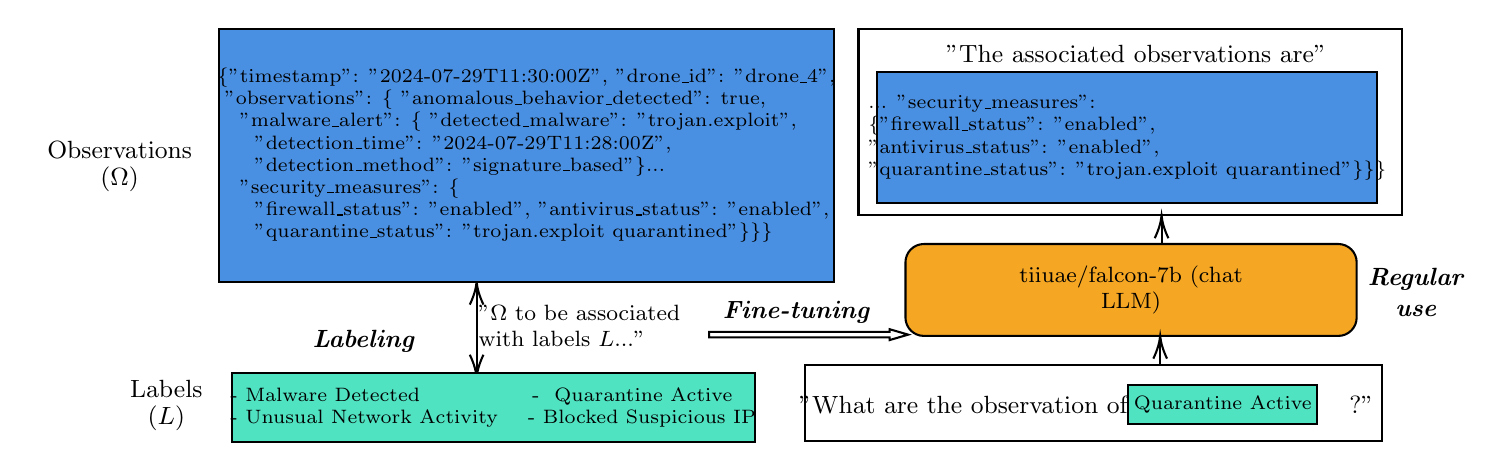
\begin{tikzpicture}[x=0.75pt,y=0.75pt,yscale=-1,xscale=1]
%uncomment if require: \path (0,1662); %set diagram left start at 0, and has height of 1662

%Rounded Rect [id:dp17386115134623514] 
\draw  [fill={rgb, 255:red, 245; green, 166; blue, 35 }  ,fill opacity=1 ] (424.61,402.58) .. controls (424.61,397.69) and (428.57,393.73) .. (433.46,393.73) -- (633.15,393.73) .. controls (638.04,393.73) and (642,397.69) .. (642,402.58) -- (642,429.15) .. controls (642,434.04) and (638.04,438) .. (633.15,438) -- (433.46,438) .. controls (428.57,438) and (424.61,434.04) .. (424.61,429.15) -- cycle ;
%Straight Lines [id:da8877910798706699] 
\draw    (547.33,451.83) -- (547.33,440) ;
\draw [shift={(547.33,438)}, rotate = 90] [color={rgb, 255:red, 0; green, 0; blue, 0 }  ][line width=0.75]    (10.93,-3.29) .. controls (6.95,-1.4) and (3.31,-0.3) .. (0,0) .. controls (3.31,0.3) and (6.95,1.4) .. (10.93,3.29)   ;
%Shape: Rectangle [id:dp44726237549140535] 
\draw   (376,452.18) -- (654,452.18) -- (654,488.66) -- (376,488.66) -- cycle ;
%Shape: Rectangle [id:dp2820683536345354] 
\draw   (402,290.27) -- (664,290.27) -- (664,379.64) -- (402,379.64) -- cycle ;
%Right Arrow [id:dp4162270206865013] 
\draw   (330,436.09) -- (417,436.09) -- (417,434.78) -- (425.91,437.39) -- (417,440) -- (417,438.7) -- (330,438.7) -- cycle ;
%Straight Lines [id:da8267677953106705] 
\draw    (548,393.83) -- (548,382) ;
\draw [shift={(548,380)}, rotate = 90] [color={rgb, 255:red, 0; green, 0; blue, 0 }  ][line width=0.75]    (10.93,-3.29) .. controls (6.95,-1.4) and (3.31,-0.3) .. (0,0) .. controls (3.31,0.3) and (6.95,1.4) .. (10.93,3.29)   ;
%Straight Lines [id:da6319519397458309] 
\draw    (218,456) -- (218,414) ;
\draw [shift={(218,412)}, rotate = 90] [color={rgb, 255:red, 0; green, 0; blue, 0 }  ][line width=0.75]    (10.93,-3.29) .. controls (6.95,-1.4) and (3.31,-0.3) .. (0,0) .. controls (3.31,0.3) and (6.95,1.4) .. (10.93,3.29)   ;
\draw [shift={(218,458)}, rotate = 270] [color={rgb, 255:red, 0; green, 0; blue, 0 }  ][line width=0.75]    (10.93,-3.29) .. controls (6.95,-1.4) and (3.31,-0.3) .. (0,0) .. controls (3.31,0.3) and (6.95,1.4) .. (10.93,3.29)   ;


% Text Node
\draw (68.5,471.5) node  [font=\footnotesize] [align=left] {\begin{minipage}[lt]{35.92pt}\setlength\topsep{0pt}
\begin{center}
{\small Labels ($\displaystyle L$)}
\end{center}

\end{minipage}};
% Text Node
\draw (372.5,426.5) node  [font=\small] [align=left] {\textit{\textbf{Fine-tuning}}};
% Text Node
\draw  [fill={rgb, 255:red, 74; green, 144; blue, 226 }  ,fill opacity=1 ]  (411,311) -- (652,311) -- (652,374) -- (411,374) -- cycle  ;
\draw (531.5,342.5) node  [font=\scriptsize] [align=left] {... "security\_measures":\\\{"firewall\_status": "enabled",\\"antivirus\_status": "enabled",\\"quarantine\_status": "trojan.exploit quarantined"\}\}\}};
% Text Node
\draw  [fill={rgb, 255:red, 80; green, 227; blue, 194 }  ,fill opacity=1 ]  (532,461.66) -- (623,461.66) -- (623,480.66) -- (532,480.66) -- cycle  ;
\draw (577.5,471.16) node  [font=\scriptsize] [align=left] {Quarantine Active};
% Text Node
\draw (536,302.25) node  [font=\footnotesize] [align=left] {{\small "The associated observations are"}};
% Text Node
\draw (671,417) node  [font=\small] [align=left] {\begin{minipage}[lt]{36.9pt}\setlength\topsep{0pt}
\begin{center}
\textit{\textbf{Regular}}\\\textit{\textbf{use}}
\end{center}

\end{minipage}};
% Text Node
\draw (512,471.16) node  [font=\footnotesize] [align=left] {{\small "What are the observation of \ \ \ \ \ \ \ \ \ \ \ \ \ \ \ \ \ \ \ \ \ \ \ \ \ ?"}};
% Text Node
\draw (46,356.32) node  [font=\footnotesize] [align=left] {\begin{minipage}[lt]{59.79pt}\setlength\topsep{0pt}
\begin{center}
{\small Observations ($\displaystyle \Omega $)}
\end{center}

\end{minipage}};
% Text Node
\draw (164,440.5) node  [font=\small] [align=left] {\textit{\textbf{Labeling}}};
% Text Node
\draw (267.5,433) node  [font=\footnotesize] [align=left] {{\footnotesize "$\displaystyle \Omega $ to be associated}\\{\footnotesize with labels $\displaystyle L$..."}};
% Text Node
\draw (533.3,415.86) node  [font=\footnotesize] [align=left] {\begin{minipage}[lt]{99.33pt}\setlength\topsep{0pt}
\begin{center}
tiiuae/falcon-7b (chat LLM)
\end{center}

\end{minipage}};
% Text Node
\draw  [fill={rgb, 255:red, 80; green, 227; blue, 194 }  ,fill opacity=1 ]  (100,456) -- (352,456) -- (352,489) -- (100,489) -- cycle  ;
\draw (226,472.5) node  [font=\scriptsize] [align=left] {\mbox{-} Malware Detected \ \ \ \ \ \ \ \ \ \ \ \ \ \ - \ Quarantine Active\\\mbox{-} Unusual Network Activity \ \ \ - Blocked Suspicious IP};
% Text Node
\draw  [fill={rgb, 255:red, 74; green, 144; blue, 226 }  ,fill opacity=1 ]  (94,290) -- (390,290) -- (390,412) -- (94,412) -- cycle  ;
\draw (242,351) node  [font=\scriptsize] [align=left] {\{"timestamp": "2024-07-29T11:30:00Z", "drone\_id": "drone\_4",\\ \ "observations": \{ "anomalous\_behavior\_detected": true,\\ \ \ \ "malware\_alert": \{ "detected\_malware": "trojan.exploit",\\ \ \ \ \ \ "detection\_time": "2024-07-29T11:28:00Z",\\ \ \ \ \ \ "detection\_method": "signature\_based"\}...\\ \ \ \ "security\_measures": \{\\ \ \ \ \ \ "firewall\_status": "enabled", "antivirus\_status": "enabled",\\ \ \ \ \ \ "quarantine\_status": "trojan.exploit quarantined"\}\}\}};


\end{tikzpicture}
    \caption{Formation et utilisation du LLM pour l'application du CoPRAHOM au 3e défi CAGE}\label{fig:llm_process}
\end{figure*}


Nous avons mis en œuvre et évalué deux modèles organisationnels à l'aide du modèle \textit{MASCARA-$\mathcal{M}OISE^+$} et adaptés à l'environnement du 3e défi CAGE de CybORG :

Le modèle « \textbf{Active Defense} » met en œuvre des mesures proactives pour anticiper, détecter et atténuer les menaces. Il vise à maintenir la sécurité et la fonctionnalité du réseau grâce à trois rôles prédéfinis :
%
\textit{Évaluateur des menaces} : surveille le réseau et identifie les menaces potentielles à l'aide d'analyses avancées ;
\textit{Stratège en réponse} : supervise les stratégies de réponse visant à neutraliser les menaces identifiées ;
\textit{Gardien du réseau} : garantit l'intégrité et la disponibilité du réseau en mettant en œuvre des mesures de sécurité.
%
Ce modèle comprend également la mission « Détection proactive des menaces », qui comprend des objectifs de détection précoce des menaces à l'aide d'analyses prédictives.

La « \textbf{Isolation des éléments suspects} » met l'accent sur l'identification et l'isolation des éléments compromis du réseau afin de contenir les menaces grâce à trois rôles :
%
\textit{Détecteur d'anomalies} : identifie les anomalies indiquant des violations potentielles ;
\textit{Spécialiste de l'isolation} : isole les systèmes compromis afin d'empêcher la propagation des menaces ;
\textit{Intervenant en cas d'incident} : coordonne la réponse et exécute les protocoles d'isolement.
%
Ce modèle comprend également la mission \textit{Détection des drones compromis}, qui comprend des objectifs visant à détecter les drones compromis et à les isoler du réseau, ainsi que la mission \textit{Confinement et isolation}, qui comprend des objectifs visant à isoler les systèmes compromis du réseau.

De plus, nous avons établi un modèle non basé sur MASCARA appelé « \textbf{Manuel} » à partir de notre compréhension empirique de l'environnement, qui sert de modèle de référence.
Nous avons également pris en compte un cas totalement sans contrainte, appelé « \textbf{Libre} », qui sert de référence MARL standard à des fins de comparaison.


\subsection{Procédure expérimentale}

Nous avons formé chaque modèle organisationnel à l'aide du \textit{CoPRAHOM Wrapper} avec le simulateur \textit{CybORG} fourni. Le wrapper intègre les spécifications et les contraintes organisationnelles pendant l'apprentissage, permettant aux agents d'apprendre et d'adapter leur comportement en fonction de rôles et de missions prédéfinis.

Nous avons sélectionné l'algorithme MAPPO pour son efficacité éprouvée dans des environnements multi-agents coopératifs sans nécessiter de modifications algorithmiques ou d'architectures spécifiques au domaine~\cite{Yu2022}. Nous avons utilisé le modèle d'algorithme implémenté MAPPO fourni par MARLlib. Plus précisément, nous avons configuré le modèle MAPPO avec un réseau MLP à deux couches, comprenant 128 neurones dans la première couche et 256 dans la seconde, optimisé à l'aide d'Adam avec un taux d'apprentissage de 0,0003. Ces configurations ont été choisies sur la base d'expériences préliminaires et des modèles d'hyperparamètres affinés disponibles dans MARLlib. Nous avons lancé l'entraînement sur 70 itérations (chacune comprenant 128 épisodes) selon un mode d'apprentissage centralisé et d'exécution décentralisée.\\

Pour former le LLM avec \texttt{ol\_mngr}, nous avons exploré l'environnement manuellement, étape par étape, à l'aide de politiques contrôlées. Cette approche a permis à l'agent de rencontrer les situations les plus pertinentes pour détecter et atténuer les programmes malveillants. Il s'agit par exemple de situations dans lesquelles un agent reçoit des messages que nous jugeons suspects ou dans lesquelles un agent reçoit la confirmation de tuer un processus. Tout au long de cette exploration, nous avons collecté, affiché (sous forme de JSON ou de graphique), interprété et étiqueté plusieurs observations à l'aide de quelques mots-clés. Cet étiquetage permet d'identifier facilement les comportements collectifs sur la base d'observations visuelles, ce qui permet de mieux contrôler les actions des agents. L'ensemble du processus de formation et d'utilisation est résumé dans \autoref{fig:llm_process}.

\subsection{Mesures d'évaluation}

Nous avons utilisé divers indicateurs pour mesurer l'impact de CoPRAHOM pendant et après la formation :
\begin{itemize}
    \item \textbf{Évolutivité} : évalue la capacité à gérer un nombre croissant d'agents et d'obstacles en fonction de l'utilisation des ressources informatiques.
    \item \textbf{Temps de convergence} : nombre d'épisodes nécessaires à l'algorithme pour atteindre une solution stable. Des temps de convergence plus courts indiquent un apprentissage plus rapide.
    \item \textbf{Écart type} : indique la variabilité des récompenses obtenues par les agents. Un écart type plus faible signifie des performances plus régulières et une organisation potentiellement plus stable.
    \item \textbf{Récompense moyenne} : La récompense moyenne obtenue par épisode reflète la performance globale de l'algorithme.
    \item \textbf{Respect des contraintes} : Évalue dans quelle mesure les agents respectent les contraintes organisationnelles données. %Il est calculé comme l'inverse du nombre de fois où les contraintes ne sont pas respectées. Un respect élevé des contraintes signifie que les agents suivent efficacement les règles.
\end{itemize}

Nous avons également inclus ces deux indicateurs spécifiques à la cyberdéfense :
\begin{itemize}
    \item \textbf{Pourcentage moyen de drones infectés par des logiciels malveillants} : mesure la proportion de drones infectés par des logiciels malveillants pendant la simulation.
    \item \textbf{Pourcentage moyen d'attaques de logiciels malveillants réussies} : indique le taux de réussite des attaques contre l'essaim de drones.
\end{itemize}

\subsection{Critères de validation}

À l'aide des indicateurs susmentionnés, nous avons défini des critères pour évaluer l'amélioration de la cyberdéfense fournie par CoPRAHOM par rapport à l'apprentissage MARL classique, en mettant particulièrement l'accent sur le modèle « défense active ». Ces critères sont les suivants :

\begin{itemize}
    \item $\mathbf{C_1}$ : Nous nous attendons à observer manuellement certaines stratégies collectives, telles que l'isolation des activités suspectes ou la coordination des manœuvres défensives.
    \item $\mathbf{C_2}$ : Nous nous attendons à une convergence plus rapide dans les modèles « Active Defense » ou « Suspect Isolation » que dans le cas « Free », et à une courbe d'apprentissage constante dans le cas « Manual ».
    \item $\mathbf{C_3}$ : Nous nous attendons à des récompenses plus élevées dans les modèles « Active Defense » ou « Suspect Isolation » par rapport au cas « Free ».
    \item $\mathbf{C_{4}}$ : Nous nous attendons à ce que l'écart type diminue entre les modèles « Libre » et « Défense active » ou « Isolation des suspects », puis entre les modèles « Défense active » ou « Isolation des suspects » et le modèle « Manuel », car les agents sont de plus en plus contraints dans leur comportement.
    \item $\mathbf{C_{5}}$ : Nous nous attendons à ce que le respect des contraintes soit entièrement couvert dans les modes \textit{correct} et \textit{correct\_policy}, mais pas dans le mode \textit{penalize}.
    \item $\mathbf{C_{6}}$ : Nous nous attendons à ce que l'évolutivité soit gérée dans tous les cas.
    \item $\mathbf{C_7}$ : Pourcentage moyen inférieur de drones infectés dans les modèles « Active Defense » ou « Suspect Isolation » par rapport au cas « Free ».
    \item $\mathbf{C_8}$ : Pourcentage moyen d'attaques de logiciels malveillants réussies inférieur dans les modèles « Active Defense » ou « Suspect Isolation » par rapport au cas « Free ».

\end{itemize}

\section{Résultats et discussion}\label{sec:results_and_discussion}

\autoref{fig:learning_curves} illustre les courbes d'apprentissage des modèles « Suspect Isolation », « Active Defensive » et « Manual », indiquant leurs taux de convergence au cours des épisodes d'entraînement.
\autoref{tab:metrics_comparison} résume le temps de convergence pendant l'entraînement ainsi que les récompenses moyennes, l'écart type, le nombre moyen de drones infectés et le nombre moyen d'attaques de logiciels malveillants obtenus par les modèles après une douzaine d'épisodes d'entraînement.

\begin{figure}[ht]
    \centering
    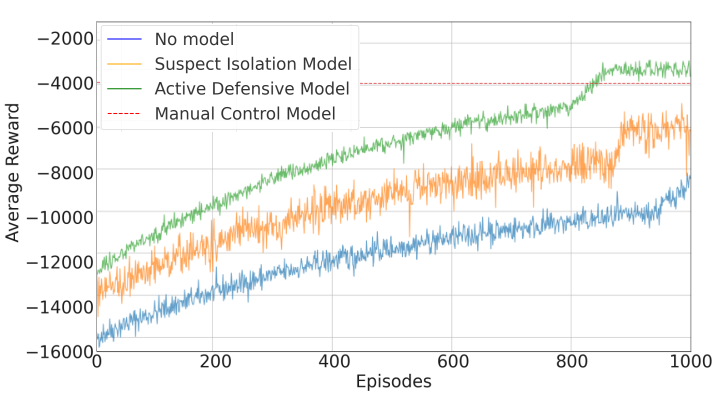
\includegraphics[width=1\linewidth]{figures/learning_curves.png}
    \caption{Courbes d'apprentissage pour \textit{Gratuit}, \textit{Isolation suspecte}, \textit{Défense active}, \textit{Manuel} en utilisant le mode \textit{correct\_policy} }
    \label{fig:learning_curves}
\end{figure}

\begin{table*}[t]
    \centering
    \setlength{\tabcolsep}{4.5pt}
    \caption{Comparaison des modèles et des modes de contrainte par rapport aux métriques.}
    \label{tab:metrics_comparison}
    \begin{tabular}{lcccccccccccc}
                                                         & {Gratuit}   & \multicolumn{3}{c}{Isolation des suspects} & \multicolumn{3}{c}{Défense active} & {Manuel}                                                                                     \\
        % \cline{2-13}
        Métrique                                         &             & Pénaliser                                  & Corriger                           & Corriger\_Politique & Pénaliser & Corriger & Corriger\_Politique &                           \\
        \midrule
        Récompense moyenne                               & -8727,49    & -5900,00                                   & -6085,12                           & -6088,00            & -3055,36  & -3100,00 & -3060,00            & -3906,00                  \\
        Écart type                                       & 138,00      & 2148,0                                     & 2027,0                             & 2018,00             & 962,      & 940,00   & 945,00              & 570,33                    \\
        Évolutivité                                      & Moyenne     & Élevée                                     & Moyenne                            & Moyenne             & Élevée    & Moyenne  & Moyenne             & Moyenne                   \\
        Temps de convergence                             &             & gt;1000                                    & 1000                               & 950                 & 950       & 800      & 850                 & 850         & $\emptyset$ \\
        Respect des contraintes                          & $\emptyset$ & Faible                                     & Élevé                              & Élevé               & Moyen     & Élevé    & Élevé               & $\emptyset$               \\
        Moyenne inf. drones (\%)                         & 61,0        & 43,0                                       & 30,0                               & 23,0                & 24,0      & 25,0     & 20,0                & 40,0                      \\
        Attaques de logiciels malveillants moyennes (\%) & 72,0        & 55,0                                       & 52,0                               & 45,0                & 38,0      & 45,0     & 40,0                & 51,0                      \\
    \end{tabular}
\end{table*}

Les modèles organisationnels ont efficacement influencé le comportement des drones dans l'environnement CybORG CAGE Challenge 3. Le modèle « Suspect Isolation » (isolement des suspects) a démontré son efficacité dans l'identification et l'isolement des drones présentant des activités suspectes, renforçant ainsi la sécurité globale. Ce modèle a permis d'identifier et de neutraliser rapidement les menaces potentielles, empêchant ainsi la propagation d'activités malveillantes au sein du essaim de drones ($\mathbf{C_1}$).

\autoref{fig:learning_curves} fournit une vue d'ensemble des courbes d'apprentissage pour chaque modèle. Le modèle « Free » (bleu) a présenté la convergence la plus lente et les récompenses moyennes les plus faibles. De plus, il montre également une faible variabilité des récompenses, ce qui indique que les agents sont lentement formés avec des changements limités à chaque étape. Ce résultat est prévisible, car le taux d'apprentissage pour MAPPO est relativement faible.

En revanche, le modèle « Suspect Isolation » (orange) a montré une convergence plus rapide et des récompenses moyennes plus élevées que le modèle « Free ». Cependant, la variabilité accrue (par rapport au modèle « Free ») suggère que, comme les agents sont contraints/incités à respecter certaines règles pour identifier et isoler les activités suspectes, leurs politiques peuvent nécessiter un certain temps pour s'habituer à ces règles et atteindre un comportement plus stable.

Le modèle « Active Defense » (vert) a affiché les récompenses moyennes les plus élevées et la convergence la plus rapide parmi tous les modèles. L'augmentation constante des récompenses démontre l'efficacité des stratégies de défense proactive mises en œuvre par les agents. Ce modèle a montré la plus grande amélioration des performances, soulignant les avantages de l'utilisation de contraintes organisationnelles structurées pour guider le comportement des agents. Le modèle « Active Defense » présente également une variabilité des récompenses plus faible que le modèle « Suspect Isolation », mais plus élevée que le modèle « Free ». Cela suggère que, même si les agents sont encore en phase d'adaptation aux contraintes, leurs comportements possibles sont plus limités dans le modèle « Active Defense » que dans le modèle « Suspect Isolation ».

Le modèle « Manuel » (ligne rouge en pointillés) a servi de référence pour la comparaison. Il a obtenu de meilleurs résultats que les modèles « Libre » et « Isolation des suspects », mais a été surpassé par le modèle « Défense active ». Cela s'explique par le fait que la stratégie de contrôle manuel, bien qu'efficace, manquait de l'adaptabilité et de l'efficacité fournies par les modèles organisationnels appris.

D'un point de vue quantitatif, les mesures fournissent également des preuves des avantages liés à l'application de contraintes organisationnelles. Comme l'illustre la figure \autoref{fig:learning_curves}, dans le cas d'une politique contrainte, les agents ont convergé plus rapidement que dans le modèle « Libre » dans tous les modes. Cela confirme que les contraintes organisationnelles peuvent accélérer l'apprentissage ($\mathbf{C_2}$). Comme prévu, la politique élaborée manuellement a permis une convergence immédiate, en raison de l'absence d'apprentissage.

Les mesures de récompense moyenne révèlent que les agents guidés par le modèle « Suspect Isolation » ont systématiquement surpassé ceux du modèle « Free », obtenant des récompenses plus élevées ($\mathbf{C_3}$). Cela indique que les contraintes organisationnelles améliorent non seulement l'efficacité de l'apprentissage, mais aussi les performances globales. Les politiques élaborées manuellement ont systématiquement obtenu les récompenses les plus élevées, soulignant l'efficacité de contraintes bien définies.

En ce qui concerne les modèles contraints, l'écart type dans \autoref{tab:metrics_comparison} a diminué progressivement du modèle le moins contraint, tel que « Suspect Isolation », au modèle le plus contraint, tel que « Active Defense » ($\mathbf{C_4}$). Cette réduction de la variabilité suggère que les contraintes organisationnelles contribuent à un comportement plus stable et plus cohérent des agents.

Le critère de respect des contraintes a été pleinement satisfait dans les modes \textit{correct} et \textit{correct\_policy}, mais pas dans le mode \textit{penalize} ($\mathbf{C_5}$). Cela démontre que si les agents peuvent apprendre à respecter efficacement les contraintes, le mode d'intégration des contraintes joue un rôle crucial. Dans notre évaluation, les modes « correct » et « correct\_policy » ont démontré une adhésion totale aux contraintes organisationnelles, comme en témoigne l'absence totale de déviations dans le comportement des agents par rapport aux rôles et missions prescrits. En revanche, le mode « pénaliser » a montré des déviations occasionnelles, en particulier dans les modèles peu contraints tels que « Suspect Isolation ». Cela suggère que les agents privilégient parfois la maximisation des récompenses plutôt que le respect strict des contraintes. Une analyse plus approfondie des stratégies de pénalisation permettrait d'améliorer la conformité.

L'évolutivité, évaluée en analysant les performances du système lorsque le nombre d'agents et d'obstacles augmente, a été gérée efficacement dans tous les modèles ($\mathbf{C_6}$). En particulier, le mode \textit{penalize} a montré une évolutivité supérieure grâce à un calcul efficace intégré des mises à jour des politiques, contrairement aux modes \textit{correct} et \textit{correct\_policy} qui nécessitent des fonctions de correction supplémentaires.

Les modèles « Active Defense » et « Suspect Isolation » ont tous deux eu un impact sur les indicateurs « Pourcentage moyen de drones infectés » et « Pourcentage moyen d'attaques de logiciels malveillants réussies » ($\mathbf{C_7}$ et $\mathbf{C_8}$). Cependant, il est important de noter que ces deux indicateurs ne sont pas directement liés à la récompense globale, car ils sont calculés séparément. Le modèle « Active Defense » a obtenu les meilleurs résultats, réduisant le pourcentage de drones infectés à 23 % et le taux de réussite des attaques de logiciels malveillants à 38 %. Cette réduction significative, comparée au taux d'infection de 61 % et au taux de réussite de 72 % du modèle « Free », démontre l'efficacité des stratégies défensives proactives dans la prévention de la propagation des logiciels malveillants et des attaques réussies. Le modèle « Isolation des suspects » a également affiché des taux d'infection et de réussite des attaques inférieurs à ceux du modèle « Libre ».

% Ces résultats soulignent l'importance de mettre en œuvre des contraintes organisationnelles structurées et des mécanismes de défense proactifs au sein des systèmes autonomes. L'intégration des modèles organisationnels $\mathcal{M}OISE^+$ dans le cadre MARL, comme le démontre CoPRAHOM, améliore considérablement l'efficacité et la coordination des agents de cyberdéfense autonomes. Les résultats expérimentaux soulignent que les contraintes organisationnelles structurées améliorent non seulement les performances et la stabilité des agents, mais garantissent également que leur comportement est conforme aux objectifs de la mission et aux objectifs de cybersécurité.

% Les résultats suggèrent qu'un affinement des spécifications organisationnelles et l'intégration de règles et de protocoles plus sophistiqués pourraient améliorer encore davantage le comportement et la coordination des agents. Ce développement continu promet de renforcer la résilience et la robustesse des stratégies de cyberdéfense face à des menaces de plus en plus sophistiquées.
% Cependant, la généralisation de CoPRAHOM à différents scénarios de cyberdéfense réels, tels que la sécurité de l'IoT ou les systèmes de contrôle industriel, pourrait nécessiter des ajustements des spécifications organisationnelles et des contraintes politiques. Les travaux futurs devraient explorer ces adaptations afin de valider la large applicabilité de CoPRAHOM.

\section{Conclusion}\label{sec:conclusion}

Notre contribution est motivée par le coût élevé de la conception de systèmes multi-agents de cyberdéfense (MAS) dans divers scénarios, en particulier lorsqu'il s'agit de faire face à des menaces en constante évolution. Pour remédier à ce problème, nous proposons un algorithme dédié appelé CoPRAHOM, qui exploite l'apprentissage par renforcement multi-agents (MARL) en fonction des spécifications organisationnelles. CoPRAHOM garantit le respect de certaines contraintes dans le comportement des agents, ce qui facilite la surveillance et la compréhension des agents formés.

CoPRAHOM a été évalué à l'aide de notre implémentation PoC proposée pour le 3e défi CAGE, un scénario coopératif de cyberdéfense par essaim de drones conçu pour limiter/éliminer les programmes malveillants et leur impact. Nous avons établi divers modèles organisationnels, allant de modèles minimalement contraints à des modèles entièrement contraints. Nous avons évalué les stratégies collectives émergentes, affinées ou prédéfinies sur la base de critères de performance pendant et après la formation.

Les résultats indiquent que les modèles équilibrés en termes de contraintes, tels que le « modèle défensif actif », permettent d'obtenir un compromis significatif entre les contraintes et l'apprentissage autonome. Ce modèle utilise des règles prédéfinies simples pour détecter et traiter les menaces lorsque les observations sont sans ambiguïté, tout en permettant à l'agent d'apprendre à réagir dans d'autres scénarios.

Outre la contrainte des agents en fonction des spécifications organisationnelles, nous souhaitons prendre en compte des mécanismes d'explicabilité afin de comprendre les nouveaux modèles organisationnels appris. L'idée d'une amélioration itérative entre l'entraînement et l'explicabilité pourrait grandement bénéficier de l'apprentissage hiérarchique, qui aide à caractériser et à mettre en évidence les stratégies pendant l'apprentissage.
%En outre, si les premiers résultats obtenus avec LLM montrent qu'il s'agit d'un outil complémentaire prometteur pour CoPRAHOM, il pourrait également offrir de nouvelles pistes pour expliquer les comportements collectifs, en particulier dans les scénarios de cyberdéfense où la plupart des environnements en réseau ne sont pas représentables de manière visuelle ou intuitive.

% Enfin, nous visons également à améliorer l'applicabilité de PRAHOM en développant des interfaces dédiées autour de PRAHOM afin de le rendre plus accessible aux contextes industriels et de recherche.


\section{Architecture de microservices}

% TODO : A ajouter comme le cas d'étude "Architecture de microservices"
% \usepackage{cite}
% \usepackage{amsmath,amssymb,amsfonts}
% \usepackage{algorithmic}
% \usepackage{graphicx}
% \usepackage{textcomp}
% \usepackage{xcolor}

% \usepackage{amsmath,amssymb,amsfonts}
% \usepackage{algorithmic}
% \usepackage{graphicx}
% \usepackage[inline, shortlabels]{enumitem}
% \usepackage{tabularx}
% \usepackage{caption}
% \usepackage{titlesec}
% \usepackage[T2A,T1]{fontenc}
% \usepackage[english]{babel}
% \captionsetup{font=it}
% \usepackage{ragged2e}
% \addto\extrasenglish{%
%   \renewcommand{\sectionautorefname}{Section}%
%   \renewcommand{\subsectionautorefname}{Subsection}%
%   \renewcommand{\subsubsectionautorefname}{Subsubsection}%
%   \renewcommand{\tableautorefname}{Table}%
%   \renewcommand{\figureautorefname}{Figure}%
% }
% \usepackage{pifont}
% \newcommand{\cmark}{\ding{51}}%
% \newcommand{\xmark}{\ding{55}}%
% \usepackage{footmisc}
% \usepackage{multirow}

% % --- Tickz
% \usepackage{physics}
% \usepackage{amsmath}
% \usepackage{tikz}
% \usepackage{mathdots}
% \usepackage{yhmath}
% \usepackage{float}
% \usepackage{pdfpages}
% \usepackage{stfloats}
% \usepackage{cancel}
% \usepackage{color}
% \usepackage{siunitx}
% \usepackage{array}
% \usepackage{multirow}
% \usepackage{amssymb}
% \usepackage{gensymb}
% \usepackage{tabularx}
% \usepackage{extarrows}
% \usepackage{booktabs}
% \usetikzlibrary{fadings}
% \usetikzlibrary{patterns}
% \usetikzlibrary{shadows.blur}
% \usetikzlibrary{shapes}

% % ---------

% \usepackage{pdfpages}
% \usepackage{booktabs}
% \usepackage{csquotes}
% \usepackage{lipsum}  
% \usepackage{arydshln}
% \usepackage{smartdiagram}
% \usepackage[inkscapeformat=png]{svg}
% \usepackage{textcomp}
% \usepackage{tabularray}\UseTblrLibrary{varwidth}
% \usepackage{xcolor}
% \def\BibTeX{{\rm B\kern-.05em{\sc i\kern-.025em b}\kern-.08em
%     T\kern-.1667em\lower.7ex\hbox{E}\kern-.125emX}}
% \usepackage{cite}
% \usepackage{amsmath}
% \newcommand{\probP}{\text{I\kern-0.15em P}}
% \usepackage{etoolbox}
% \patchcmd{\thebibliography}{\section*{\refname}}{}{}{}

% \usepackage{hyperref}
% \setlength{\extrarowheight}{2.5pt}

% % \renewcommand{\arraystretch}{1.7}

% % \setlength{\extrarowheight}{2.5pt}
% % \renewcommand{\arraystretch}{0.2}
% % \renewcommand{\arraystretch}{1.7}

% % --------------
% \titleclass{\subsubsubsection}{straight}[\subsection]

% \newcounter{subsubsubsection}[subsubsection]
% \renewcommand\thesubsubsubsection{\thesubsubsection.\arabic{subsubsubsection}}
% \renewcommand\theparagraph{\thesubsubsubsection.\arabic{paragraph}} % optional; useful if paragraphs are to be numbered

% \titleformat{\subsubsubsection}
%   {\normalfont\normalsize\bfseries}{\thesubsubsubsection}{1em}{}
% \titlespacing*{\subsubsubsection}
% {0pt}{3.25ex plus 1ex minus .2ex}{1.5ex plus .2ex}

% \makeatletter
% \renewcommand\paragraph{\@startsection{paragraph}{5}{\z@}%
%   {3.25ex \@plus1ex \@minus.2ex}%
%   {-1em}%
%   {\normalfont\normalsize\bfseries}}
% \renewcommand\subparagraph{\@startsection{subparagraph}{6}{\parindent}%
%   {3.25ex \@plus1ex \@minus .2ex}%
%   {-1em}%
%   {\normalfont\normalsize\bfseries}}
% \def\toclevel@subsubsubsection{4}
% \def\toclevel@paragraph{5}
% \def\toclevel@paragraph{6}
% \def\l@subsubsubsection{\@dottedtocline{4}{7em}{4em}}
% \def\l@paragraph{\@dottedtocline{5}{10em}{5em}}
% \def\l@subparagraph{\@dottedtocline{6}{14em}{6em}}
% \makeatother

% \makeatletter
% \newcommand{\linebreakand}{%
%   \end{@IEEEauthorhalign}
%   \hfill\mbox{}\par
%   \mbox{}\hfill\begin{@IEEEauthorhalign}
% }
% \makeatother

% \setcounter{secnumdepth}{4}
% \setcounter{tocdepth}{4}


% \setboolean{@twoside}{false}

% % --------------


% \newcommand{\before}[1]{\textcolor{red}{#1}}
% \newcommand{\after}[1]{\textcolor{green}{#1}}

% \newcommand{\old}[1]{\textcolor{orange}{#1}}
% \newcommand{\rem}[1]{\textcolor{red}{#1}}
% \newcommand{\todo}[1]{\textcolor{orange}{\newline \textit{\textbf{TODO:} #1}} \newline \newline }

% \def\BibTeX{{\rm B\kern-.05em{\sc i\kern-.025em b}\kern-.08em
%     T\kern-.1667em\lower.7ex\hbox{E}\kern-.125emX}}

\section{Introduction}
\label{sec:introduction}

% Context
Cloud-native critical systems are increasingly reliant on Kubernetes to orchestrate and manage interdependent services~\cite{Pahl2019}. HPA is a widely adopted mechanism to dynamically adjust the number of pods based on resource usage, enabling systems to handle highly dynamic workloads~\cite{Toka2020}. However, failures such as pod crashes, resource contention, and bottlenecks can severely jeopardize the performance of all of the cluster's functionalities we globally refer to as operational resilience~\cite{burns2016borg}. Worse, these failures may be exploited by attackers to degrade performance or induce outages, as seen in adversarial contexts like DDoS attacks~\cite{David2021}.

Although DDoS attacks may seem unlikely in isolated enterprise clusters, many organizations expose services via ingress gateways, making them viable targets. Internally, DDoS-like overloads can also result from misconfigurations, compromised devices, or red-teaming exercises. Accounting for such adversarial scenarios aligns with cybersecurity best practices and helps ensure robust, fault-tolerant autoscaling.

In such adversarial scenarios, malicious actors can exploit scaling mechanisms, exposing the limitations of conventional HPA systems. Modern approaches have sought to address these gaps using Reinforcement Learning (RL), where an agent optimizes a single global goal such as minimizing latency or resource usage~\cite{Gari2021}. While these methods demonstrate adaptability, they often fall short in handling diverse failure scenarios to maintain \textit{Quality of Service} (QoS)~\cite{Liu2024}. For example, prioritizing responses to cascading pod crashes during an attack may be far more critical than reducing latency. These challenges highlight the need for an autoscaling system capable of dynamically balancing multiple sub-goals to maintain all of the QoS to maximize operational resilience.

Achieving this shift from single-goal optimization to a multi-goal approach is complex~\cite{Shoham2009MAS}. In real-world scenarios, operational resilience is not reducible to a single objective: optimizing for low latency may conflict with ensuring high availability or limiting resource overprovisioning. During adversarial conditions, for example, prioritizing DDoS mitigation may require sacrificing latency, while pod crash recovery demands rapid reallocation of resources. A single RL agent struggles to address such priorities due to the difficulty of coordinating responses to diverse failures~\cite{Jennings1998}.

In contrast, MASs offer a promising paradigm by decomposing the overarching operational resilience maximization goal into sub-goals handled by specialized agents~\cite{Shoham2009MAS}. Each agent focuses on a specific failure mode or performance objective, which facilitates specialization, improved coordination, and scalable policy learning under dynamic workloads.

Considering an adversarial scenario, each defender can collaboratively contribute to complementary scaling actions to reach its own sub-goal, enabling more resilient and context-specific responses face to an attacker~\cite{Jennings1998}. We refer to the set of these collaborative as an HPA MAS. An HPA MAS actually builds upon the cyberdefense framework of Autonomous Intelligent Cybersecurity Agents (AICAs), which can be viewed as agents with specialized roles and missions collaboratively defending systems against attackers~\cite{Kott2018}.

% Problématique
However, designing HPA MASs tailored to a cluster presents significant challenges such as the need for detailed cluster knowledge, the time-consuming nature of manual design processes, and the difficulty of ensuring optimal agent behavior. Moreover, cluster changes require repeating the design process, increasing operational costs and complexity.

% Contribution
Among methdological works, we inspired from the \textit{Assisted MAS Organization Engineering Approach} (AOMEA)~\cite{soule2024aomea} that shows to align the most with automation and safety challenges. Based on AOMEA, we propose the \textit{Kubernetes Autoscaling with Resilient Multi-Agent system} (KARMA) to automate the design and implementation process through four sequential phases:
\begin{enumerate*}[label=\textbf{\arabic*)}, itemjoin={;\quad }]
    \item \textbf{Modeling}: Creating a digital twin of the cluster from real-world traces to simulate failure scenarios
    \item \textbf{Training}: Training agents in simulation using roles and missions that integrate explicit rule-based and guidance strategies
    \item \textbf{Analyzing}: Validating trained agents' behaviors and extracting design insights through empirical analysis
    \item \textbf{Transferring}: Running trained agents to apply their learned behaviors via the real Kubernetes API.
\end{enumerate*}

This framework enables to iteratively updates the simulation model with newly collected traces, enabling adaptation to cluster changes. We validated our approach on adversarial scenarios from the "Chained Service" Kubernetes environment. The MASs were generated with minimal manual intervention and demonstrate originality. They compete with state-of-the-art HPA systems, including AWARE~\cite{aware2023}, Gym-HPA~\cite{gymhpa2022}, and Rlad-core~\cite{Rossi2019}, in maximizing operational resilience.

% Organisation
The remainder is structured as follows:
\autoref{sec:related_work} reviews existing HPA techniques and their limitations in dynamic environments.
\autoref{sec:proposed_approach} details our framework leveraging related concepts for each phase.
\autoref{sec:experiments} describes the experimental setup.
\autoref{sec:results} presents and discusses results.
\autoref{sec:conclusion} concludes and provides future directions.

% ===================================

\section{Related Work}
\label{sec:related_work}

\begin{table}[h!]
    \centering
    \caption{A KARMA overview regarding selected HPA Systems}
    \label{tab:autoscaling_criteria}
    {\footnotesize
    \renewcommand{\arraystretch}{1.1}
    % \resizebox{0.5\textwidth}{!}{%
    \begin{tabular}{>{\raggedright\arraybackslash}m{1.3cm}>{\centering\arraybackslash}m{0.6cm}>{\centering\arraybackslash}m{0.6cm}>{\centering\arraybackslash}m{0.6cm}>{\centering\arraybackslash}m{0.6cm}>{\centering\arraybackslash}m{0.6cm}>{\centering\arraybackslash}m{0.6cm}>{\centering\arraybackslash}m{0.6cm}>{\centering\arraybackslash}m{0.6cm}>{\centering\arraybackslash}m{0.6cm}}
    \hline
    \textbf{Criterion} & \vspace{-0.3cm}\textbf{\cite{gymhpa2022}} & \vspace{-0.3cm}\textbf{\cite{aware2023}} & \vspace{-0.3cm}\textbf{\cite{Rossi2019}} & \vspace{-0.3cm}\textbf{\cite{QoSRL}} & \vspace{-0.3cm}\textbf{\cite{Zhou2024}} & \vspace{-0.3cm}\textbf{\cite{KOSMOS}} & \vspace{-0.3cm}\textbf{\cite{COPA}} \\
    \hline
    \hline
    Adversarial Scenarios & No & Partial & No & No & No & No & Partial \\
    \hline
    Multi-goal & No & Yes & Partial & Yes & No & Yes & No \\
    \hline
    Automation & High & Mid. & Mid. & High & Mid. & Mid. & Mid. \\
    \hline
    Learning & Yes & Yes & Yes & Yes & No & No & No \\
    \hline
    MAS & No & No & No & No & No & No & No \\
    \hline
    Simulation & Yes & No & Yes & Yes & No & No & No \\
    \hline
    Real env. & No & Yes & Yes & Yes & Yes & Yes & Yes \\
    \hline
    Explainable & No & No & No & No & No & No & No \\
    \hline
    Adaptation & High & Mid. & Mid. & Mid. & High & High & Mid. \\
    \hline
    Safety Guarantees & No & No & No & No & No & No & No \\
    \hline
    \end{tabular}%
    }
  \end{table}


\noindent Autoscaling in Kubernetes has traditionally relied on metrics-based approaches, such as the default Kubernetes Horizontal Pod Autoscaler (KHPA), which adjusts the number of pods based on CPU and memory utilization~\cite{Carrion2022}. While effective for basic scaling, such methods fail to address dynamic or adversarial workloads, as they rely on reactive, threshold-based rules~\cite{Tran2022}. To overcome these limitations, recent research has turned to Machine Learning (ML) and RL.

% \subsection*{Reinforcement Learning-Based Systems}
Three RL-based systems stand out for their innovative approaches, applicability, and relevance:
%
\begin{itemize}
    \item \textbf{Gym-HPA}~\cite{gymhpa2022} serves as a benchmark RL environment, enabling experimentation with various RL algorithms. It excels in adaptability to simulated workloads with a high degree of automation but lacks multi-goal support, explainability, and real-world applicability
    \item \textbf{AWARE}~\cite{aware2023} incorporates RL to optimize autoscaling decisions while balancing QoS goals, such as response time and throughput. It partially considers adversarial scenarios but struggles with high automation levels and multi-agent coordination
    \item \textbf{Rlad-core}~\cite{Rossi2019} focus on both horizontal and vertical scaling introducing a self-adaptive system that dynamically adjusts resource allocation in response to workload variations, optimizing performance while minimizing costs.
\end{itemize}

These systems highlight significant progress in RL-based autoscaling but share common limitations: a lack of comprehensive adversarial adaptability, limited support for MAS, and no explicit focus on explainability or safety guarantees.
%
% \subsection*{Hybrid and Rule-Based Approaches}
Other notable systems combine ML or rule-based strategies with traditional autoscaling:
%
\begin{enumerate*}[label={}, itemjoin={;\quad }]
    \item \textbf{QoS-Aware RL}~\cite{QoSRL} focus on maintaining QoS under dynamic workloads but does not integrate seamlessly with Kubernetes-native features or consider adversarial scenarios
    \item \textbf{AHPA}~\cite{Zhou2024} and \textbf{KOSMOS}~\cite{KOSMOS} explore adaptive and combined vertical-horizontal scaling strategies, offering high adaptability but lacking learning capabilities
    \item \textbf{COPA}~\cite{COPA} emphasize combined metrics-based autoscaling but remains reactive and limited in adversarial scenarios.
\end{enumerate*}

% \subsection*{Positioning Our Contribution}
KARMA addresses key gaps in \textbf{(1) operational resilience} for autoscaling by introducing an automated HPA MAS design framework. Unlike conventional approaches, which often fail under \textbf{(2) adversarial conditions}, KARMA decomposes maintaining operational resilience into failure-specific missions and roles, enabling agents to handle coordinate response to \textbf{bottlenecks}, \textbf{resource contention}, \textbf{DDoS}, and \textbf{pod crashes}. It combines \textbf{(3) digital twin modeling} with \textbf{(4) automated MAS generation} via Multi-Agent Reinforcement Learning (MARL) integrating \textbf{constraint satisfaction} to these roles and missions, streamlining HPA MAS design with minimal manual intervention. Leveraging this decomposition, KARMA seeks for a better \textbf{(5) adaptability} while also enabling a better \textbf{(6) explainability} as for decision making in the whole HPA MAS.


% ===================================
\section{KARMA: A framework for HPA MAS design and development}
\label{sec:proposed_approach}

This section overviews the KARMA framework to helps in designing a HPA MAS then details each one of its phase.

\subsection{KARMA Overview}

\begin{figure}[h!]
    \centering
    


\tikzset{every picture/.style={line width=0.75pt}} %set default line width to 0.75pt        

\begin{tikzpicture}[x=0.75pt,y=0.75pt,yscale=-1.2,xscale=1.2]
%uncomment if require: \path (0,1414); %set diagram left start at 0, and has height of 1414

%Straight Lines [id:da5609883377896374] 
\draw [color={rgb, 255:red, 74; green, 144; blue, 226 }  ,draw opacity=1 ][line width=2.25]    (317.22,111.13) -- (360.07,111.13) ;
\draw [shift={(365.07,111.13)}, rotate = 180] [fill={rgb, 255:red, 74; green, 144; blue, 226 }  ,fill opacity=1 ][line width=0.08]  [draw opacity=0] (5.72,-2.75) -- (0,0) -- (5.72,2.75) -- cycle    ;
%Image [id:dp9396292457736715] 
\draw (106.77,60.95) node  {
\includegraphics[width=18.66pt,height=18.36pt]{figures/karma_architecture/pod.png}};
%Image [id:dp3874378335758297] 
\draw (145.86,60.95) node  {
\includegraphics[width=18.66pt,height=18.36pt]{figures/karma_architecture/pod.png}};
%Shape: Rectangle [id:dp4562827234223257] 
\draw  [color={rgb, 255:red, 74; green, 144; blue, 226 }  ,draw opacity=1 ][line width=1.5]  (89,28.36) .. controls (89,25.6) and (91.24,23.36) .. (94,23.36) -- (255,23.36) .. controls (257.76,23.36) and (260,25.6) .. (260,28.36) -- (260,132) .. controls (260,134.76) and (257.76,137) .. (255,137) -- (94,137) .. controls (91.24,137) and (89,134.76) .. (89,132) -- cycle ;
%Image [id:dp9455935833751838] 
\draw (172.5,16.24) node  {
\includegraphics[width=18.66pt,height=18.36pt]{figures/karma_architecture/kubernetes.png}};
%Shape: Rectangle [id:dp9564725691593288] 
\draw  [color={rgb, 255:red, 74; green, 144; blue, 226 }  ,draw opacity=1 ][line width=1.5]  (92.55,50.21) .. controls (92.55,47.45) and (94.79,45.21) .. (97.55,45.21) -- (155.08,45.21) .. controls (157.84,45.21) and (160.08,47.45) .. (160.08,50.21) -- (160.08,70.81) .. controls (160.08,73.57) and (157.84,75.81) .. (155.08,75.81) -- (97.55,75.81) .. controls (94.79,75.81) and (92.55,73.57) .. (92.55,70.81) -- cycle ;
%Image [id:dp9120856447688912] 
\draw (126.32,39.97) node  {
\includegraphics[width=18.66pt,height=18.36pt]{figures/karma_architecture/node.png}};
%Image [id:dp5738167237736518] 
\draw (106.77,119.52) node  {
\includegraphics[width=18.66pt,height=18.36pt]{figures/karma_architecture/pod.png}};
%Image [id:dp2199681121060142] 
\draw (145.86,119.52) node  {
\includegraphics[width=18.66pt,height=18.36pt]{figures/karma_architecture/pod.png}};
%Shape: Rectangle [id:dp12159705904547402] 
\draw  [color={rgb, 255:red, 74; green, 144; blue, 226 }  ,draw opacity=1 ][line width=1.5]  (92.55,108.78) .. controls (92.55,106.02) and (94.79,103.78) .. (97.55,103.78) -- (155.08,103.78) .. controls (157.84,103.78) and (160.08,106.02) .. (160.08,108.78) -- (160.08,129.38) .. controls (160.08,132.14) and (157.84,134.38) .. (155.08,134.38) -- (97.55,134.38) .. controls (94.79,134.38) and (92.55,132.14) .. (92.55,129.38) -- cycle ;
%Image [id:dp37768653229718074] 
\draw (126.32,98.54) node  {
\includegraphics[width=18.66pt,height=18.36pt]{figures/karma_architecture/node.png}};
%Shape: Rectangle [id:dp20840815212238661] 
\draw  [color={rgb, 255:red, 74; green, 144; blue, 226 }  ,draw opacity=1 ][line width=1.5]  (264,28.36) .. controls (264,25.6) and (266.24,23.36) .. (269,23.36) -- (411.78,23.36) .. controls (414.54,23.36) and (416.78,25.6) .. (416.78,28.36) -- (416.78,132) .. controls (416.78,134.76) and (414.54,137) .. (411.78,137) -- (269,137) .. controls (266.24,137) and (264,134.76) .. (264,132) -- cycle ;
%Straight Lines [id:da9232180983272227] 
\draw [color={rgb, 255:red, 74; green, 144; blue, 226 }  ,draw opacity=1 ][line width=2.25]    (164,112) -- (201,112) ;
\draw [shift={(206,112)}, rotate = 180] [fill={rgb, 255:red, 74; green, 144; blue, 226 }  ,fill opacity=1 ][line width=0.08]  [draw opacity=0] (5.72,-2.75) -- (0,0) -- (5.72,2.75) -- cycle    ;
%Straight Lines [id:da6082715106712999] 
\draw [color={rgb, 255:red, 74; green, 144; blue, 226 }  ,draw opacity=1 ][line width=2.25]    (180,90.22) -- (167,90.22) ;
\draw [shift={(162,90.22)}, rotate = 360] [fill={rgb, 255:red, 74; green, 144; blue, 226 }  ,fill opacity=1 ][line width=0.08]  [draw opacity=0] (5.72,-2.75) -- (0,0) -- (5.72,2.75) -- cycle    ;
%Straight Lines [id:da30764510910060716] 
\draw [color={rgb, 255:red, 74; green, 144; blue, 226 }  ,draw opacity=1 ][line width=2.25]    (210,72) -- (199,72) ;
\draw [shift={(194,72)}, rotate = 360] [fill={rgb, 255:red, 74; green, 144; blue, 226 }  ,fill opacity=1 ][line width=0.08]  [draw opacity=0] (5.72,-2.75) -- (0,0) -- (5.72,2.75) -- cycle    ;
%Straight Lines [id:da5394403186779959] 
\draw [color={rgb, 255:red, 74; green, 144; blue, 226 }  ,draw opacity=1 ][line width=2.25]    (178,56.22) -- (167,56.22) ;
\draw [shift={(162,56.22)}, rotate = 360] [fill={rgb, 255:red, 74; green, 144; blue, 226 }  ,fill opacity=1 ][line width=0.08]  [draw opacity=0] (5.72,-2.75) -- (0,0) -- (5.72,2.75) -- cycle    ;
%Straight Lines [id:da6399475815904785] 
\draw [color={rgb, 255:red, 74; green, 144; blue, 226 }  ,draw opacity=1 ][line width=2.25]    (272,72) -- (235,72) ;
\draw [shift={(230,72)}, rotate = 360] [fill={rgb, 255:red, 74; green, 144; blue, 226 }  ,fill opacity=1 ][line width=0.08]  [draw opacity=0] (5.72,-2.75) -- (0,0) -- (5.72,2.75) -- cycle    ;
%Straight Lines [id:da24320102833940327] 
\draw [color={rgb, 255:red, 74; green, 144; blue, 226 }  ,draw opacity=1 ][line width=2.25]    (267,112) -- (230,112) ;
\draw [shift={(272,112)}, rotate = 180] [fill={rgb, 255:red, 74; green, 144; blue, 226 }  ,fill opacity=1 ][line width=0.08]  [draw opacity=0] (5.72,-2.75) -- (0,0) -- (5.72,2.75) -- cycle    ;
%Shape: Rectangle [id:dp9149123987409296] 
\draw  [color={rgb, 255:red, 255; green, 255; blue, 255 }  ,draw opacity=1 ][fill={rgb, 255:red, 255; green, 255; blue, 255 }  ,fill opacity=1 ] (328.83,106.67) -- (353.11,106.67) -- (353.11,114) -- (328.83,114) -- cycle ;
%Image [id:dp7127891043436136] 
\draw (341.68,109.47) node  {
\includegraphics[width=14.57pt,height=15.21pt]{figures/karma_architecture/pettingzoo.png}};
%Straight Lines [id:da5757027637146572] 
\draw [color={rgb, 255:red, 74; green, 144; blue, 226 }  ,draw opacity=1 ][line width=2.25]    (357.9,41) -- (364.9,41) ;
\draw [shift={(352.9,41)}, rotate = 0] [fill={rgb, 255:red, 74; green, 144; blue, 226 }  ,fill opacity=1 ][line width=0.08]  [draw opacity=0] (5.72,-2.75) -- (0,0) -- (5.72,2.75) -- cycle    ;
%Straight Lines [id:da29364722138505184] 
\draw [color={rgb, 255:red, 74; green, 144; blue, 226 }  ,draw opacity=1 ][line width=2.25]    (390.99,97.77) -- (390.99,57.25) ;
\draw [shift={(390.99,52.25)}, rotate = 90] [fill={rgb, 255:red, 74; green, 144; blue, 226 }  ,fill opacity=1 ][line width=0.08]  [draw opacity=0] (5.72,-2.75) -- (0,0) -- (5.72,2.75) -- cycle    ;
%Straight Lines [id:da5470457469462804] 
\draw [color={rgb, 255:red, 74; green, 144; blue, 226 }  ,draw opacity=1 ][line width=2.25]    (390.9,71) -- (325.9,71) ;
\draw [shift={(320.9,71)}, rotate = 360] [fill={rgb, 255:red, 74; green, 144; blue, 226 }  ,fill opacity=1 ][line width=0.08]  [draw opacity=0] (5.72,-2.75) -- (0,0) -- (5.72,2.75) -- cycle    ;
%Shape: Rectangle [id:dp8476965567779329] 
\draw  [color={rgb, 255:red, 255; green, 255; blue, 255 }  ,draw opacity=1 ][fill={rgb, 255:red, 255; green, 255; blue, 255 }  ,fill opacity=1 ] (378.41,65.11) -- (397.83,65.11) -- (397.83,92) -- (378.41,92) -- cycle ;
%Shape: Smiley Face [id:dp8656850497140396] 
\draw  [fill={rgb, 255:red, 255; green, 255; blue, 255 }  ,fill opacity=1 ][line width=0.75]  (380.35,69.4) .. controls (380.35,67.3) and (382.09,65.6) .. (384.24,65.6) .. controls (386.38,65.6) and (388.12,67.3) .. (388.12,69.4) .. controls (388.12,71.5) and (386.38,73.2) .. (384.24,73.2) .. controls (382.09,73.2) and (380.35,71.5) .. (380.35,69.4) -- cycle ; \draw  [fill={rgb, 255:red, 255; green, 255; blue, 255 }  ,fill opacity=1 ][line width=0.75]  (382.53,68.11) .. controls (382.53,67.9) and (382.7,67.73) .. (382.92,67.73) .. controls (383.13,67.73) and (383.31,67.9) .. (383.31,68.11) .. controls (383.31,68.32) and (383.13,68.49) .. (382.92,68.49) .. controls (382.7,68.49) and (382.53,68.32) .. (382.53,68.11) -- cycle ; \draw  [fill={rgb, 255:red, 255; green, 255; blue, 255 }  ,fill opacity=1 ][line width=0.75]  (385.17,68.11) .. controls (385.17,67.9) and (385.34,67.73) .. (385.56,67.73) .. controls (385.77,67.73) and (385.95,67.9) .. (385.95,68.11) .. controls (385.95,68.32) and (385.77,68.49) .. (385.56,68.49) .. controls (385.34,68.49) and (385.17,68.32) .. (385.17,68.11) -- cycle ; \draw  [line width=0.75]  (382.29,70.92) .. controls (383.59,71.94) and (384.88,71.94) .. (386.18,70.92) ;
%Shape: Smiley Face [id:dp9163740789669144] 
\draw  [fill={rgb, 255:red, 255; green, 255; blue, 255 }  ,fill opacity=1 ][line width=0.75]  (392.01,69.4) .. controls (392.01,67.3) and (393.75,65.6) .. (395.89,65.6) .. controls (398.04,65.6) and (399.78,67.3) .. (399.78,69.4) .. controls (399.78,71.5) and (398.04,73.2) .. (395.89,73.2) .. controls (393.75,73.2) and (392.01,71.5) .. (392.01,69.4) -- cycle ; \draw  [fill={rgb, 255:red, 255; green, 255; blue, 255 }  ,fill opacity=1 ][line width=0.75]  (394.18,68.11) .. controls (394.18,67.9) and (394.36,67.73) .. (394.57,67.73) .. controls (394.79,67.73) and (394.96,67.9) .. (394.96,68.11) .. controls (394.96,68.32) and (394.79,68.49) .. (394.57,68.49) .. controls (394.36,68.49) and (394.18,68.32) .. (394.18,68.11) -- cycle ; \draw  [fill={rgb, 255:red, 255; green, 255; blue, 255 }  ,fill opacity=1 ][line width=0.75]  (396.82,68.11) .. controls (396.82,67.9) and (397,67.73) .. (397.21,67.73) .. controls (397.43,67.73) and (397.6,67.9) .. (397.6,68.11) .. controls (397.6,68.32) and (397.43,68.49) .. (397.21,68.49) .. controls (397,68.49) and (396.82,68.32) .. (396.82,68.11) -- cycle ; \draw  [line width=0.75]  (393.95,70.92) .. controls (395.24,71.94) and (396.54,71.94) .. (397.83,70.92) ;
%Shape: Smiley Face [id:dp8186451078369623] 
\draw  [fill={rgb, 255:red, 255; green, 255; blue, 255 }  ,fill opacity=1 ][line width=0.75]  (386.18,77.44) .. controls (386.18,75.34) and (387.92,73.64) .. (390.06,73.64) .. controls (392.21,73.64) and (393.95,75.34) .. (393.95,77.44) .. controls (393.95,79.54) and (392.21,81.24) .. (390.06,81.24) .. controls (387.92,81.24) and (386.18,79.54) .. (386.18,77.44) -- cycle ; \draw  [fill={rgb, 255:red, 255; green, 255; blue, 255 }  ,fill opacity=1 ][line width=0.75]  (388.36,76.15) .. controls (388.36,75.94) and (388.53,75.77) .. (388.74,75.77) .. controls (388.96,75.77) and (389.13,75.94) .. (389.13,76.15) .. controls (389.13,76.36) and (388.96,76.53) .. (388.74,76.53) .. controls (388.53,76.53) and (388.36,76.36) .. (388.36,76.15) -- cycle ; \draw  [fill={rgb, 255:red, 255; green, 255; blue, 255 }  ,fill opacity=1 ][line width=0.75]  (391,76.15) .. controls (391,75.94) and (391.17,75.77) .. (391.39,75.77) .. controls (391.6,75.77) and (391.77,75.94) .. (391.77,76.15) .. controls (391.77,76.36) and (391.6,76.53) .. (391.39,76.53) .. controls (391.17,76.53) and (391,76.36) .. (391,76.15) -- cycle ; \draw  [line width=0.75]  (388.12,78.96) .. controls (389.42,79.98) and (390.71,79.98) .. (392.01,78.96) ;
%Flowchart: Punched Tape [id:dp6020643269389074] 
\draw  [fill={rgb, 255:red, 255; green, 255; blue, 255 }  ,fill opacity=1 ] (313.9,33.81) .. controls (313.9,35.03) and (318.18,36.02) .. (323.45,36.02) .. controls (328.73,36.02) and (333,35.03) .. (333,33.81) .. controls (333,32.58) and (337.28,31.59) .. (342.55,31.59) .. controls (347.83,31.59) and (352.1,32.58) .. (352.1,33.81) -- (352.1,51.52) .. controls (352.1,50.3) and (347.83,49.31) .. (342.55,49.31) .. controls (337.28,49.31) and (333,50.3) .. (333,51.52) .. controls (333,52.75) and (328.73,53.74) .. (323.45,53.74) .. controls (318.18,53.74) and (313.9,52.75) .. (313.9,51.52) -- cycle ;
%Straight Lines [id:da950307097731951] 
\draw [line width=0.75]    (324.14,41.04) -- (341.9,41) ;
%Shape: Smiley Face [id:dp8914579811118104] 
\draw  [line width=0.75]  (320.58,40.88) .. controls (320.58,39.7) and (321.59,38.73) .. (322.85,38.73) .. controls (324.1,38.73) and (325.11,39.7) .. (325.11,40.88) .. controls (325.11,42.07) and (324.1,43.03) .. (322.85,43.03) .. controls (321.59,43.03) and (320.58,42.07) .. (320.58,40.88) -- cycle ; \draw  [line width=0.75]  (321.85,40.15) .. controls (321.85,40.03) and (321.95,39.94) .. (322.08,39.94) .. controls (322.2,39.94) and (322.3,40.03) .. (322.3,40.15) .. controls (322.3,40.27) and (322.2,40.37) .. (322.08,40.37) .. controls (321.95,40.37) and (321.85,40.27) .. (321.85,40.15) -- cycle ; \draw  [line width=0.75]  (323.39,40.15) .. controls (323.39,40.03) and (323.49,39.94) .. (323.62,39.94) .. controls (323.74,39.94) and (323.84,40.03) .. (323.84,40.15) .. controls (323.84,40.27) and (323.74,40.37) .. (323.62,40.37) .. controls (323.49,40.37) and (323.39,40.27) .. (323.39,40.15) -- cycle ; \draw  [line width=0.75]  (321.71,41.74) .. controls (322.47,42.31) and (323.22,42.31) .. (323.98,41.74) ;
%Shape: Smiley Face [id:dp07941198495535606] 
\draw  [line width=0.75]  (329.9,45.15) .. controls (329.9,43.96) and (330.92,43) .. (332.17,43) .. controls (333.42,43) and (334.44,43.96) .. (334.44,45.15) .. controls (334.44,46.33) and (333.42,47.29) .. (332.17,47.29) .. controls (330.92,47.29) and (329.9,46.33) .. (329.9,45.15) -- cycle ; \draw  [line width=0.75]  (331.17,44.42) .. controls (331.17,44.3) and (331.28,44.2) .. (331.4,44.2) .. controls (331.53,44.2) and (331.63,44.3) .. (331.63,44.42) .. controls (331.63,44.54) and (331.53,44.63) .. (331.4,44.63) .. controls (331.28,44.63) and (331.17,44.54) .. (331.17,44.42) -- cycle ; \draw  [line width=0.75]  (332.72,44.42) .. controls (332.72,44.3) and (332.82,44.2) .. (332.94,44.2) .. controls (333.07,44.2) and (333.17,44.3) .. (333.17,44.42) .. controls (333.17,44.54) and (333.07,44.63) .. (332.94,44.63) .. controls (332.82,44.63) and (332.72,44.54) .. (332.72,44.42) -- cycle ; \draw  [line width=0.75]  (331.04,46.01) .. controls (331.79,46.58) and (332.55,46.58) .. (333.3,46.01) ;
%Shape: Smiley Face [id:dp8353415903298282] 
\draw  [line width=0.75]  (341.9,40.85) .. controls (341.9,39.67) and (342.92,38.71) .. (344.17,38.71) .. controls (345.42,38.71) and (346.44,39.67) .. (346.44,40.85) .. controls (346.44,42.04) and (345.42,43) .. (344.17,43) .. controls (342.92,43) and (341.9,42.04) .. (341.9,40.85) -- cycle ; \draw  [line width=0.75]  (343.17,40.12) .. controls (343.17,40) and (343.28,39.91) .. (343.4,39.91) .. controls (343.53,39.91) and (343.63,40) .. (343.63,40.12) .. controls (343.63,40.24) and (343.53,40.34) .. (343.4,40.34) .. controls (343.28,40.34) and (343.17,40.24) .. (343.17,40.12) -- cycle ; \draw  [line width=0.75]  (344.72,40.12) .. controls (344.72,40) and (344.82,39.91) .. (344.94,39.91) .. controls (345.07,39.91) and (345.17,40) .. (345.17,40.12) .. controls (345.17,40.24) and (345.07,40.34) .. (344.94,40.34) .. controls (344.82,40.34) and (344.72,40.24) .. (344.72,40.12) -- cycle ; \draw  [line width=0.75]  (343.04,41.71) .. controls (343.79,42.28) and (344.55,42.28) .. (345.3,41.71) ;
%Straight Lines [id:da21936285199788075] 
\draw [line width=0.75]    (324.19,41.87) -- (329.9,45) ;
%Image [id:dp05694376090002984] 
\draw (218.44,70.24) node  {
\includegraphics[width=18.66pt,height=18.36pt]{figures/karma_architecture/api.png}};
%Image [id:dp7747210194064744] 
\draw (186.74,54.54) node  {
\includegraphics[width=18.66pt,height=18.36pt]{figures/karma_architecture/deploy.png}};
%Image [id:dp5268588430037433] 
\draw (186.74,87.76) node  {
\includegraphics[width=18.66pt,height=18.36pt]{figures/karma_architecture/deploy.png}};
%Image [id:dp7447308292951857] 
\draw (218.44,111.76) node  {
\includegraphics[width=18.66pt,height=18.36pt]{figures/karma_architecture/prometheus.png}};
%Shape: Rectangle [id:dp7837974954754439] 
\draw  [color={rgb, 255:red, 75; green, 101; blue, 225 }  ,draw opacity=1 ][fill={rgb, 255:red, 74; green, 144; blue, 226 }  ,fill opacity=1 ] (202.37,94.64) -- (208.29,94.64) -- (208.29,101.67) -- (202.37,101.67) -- cycle ;
%Shape: Rectangle [id:dp780870970882084] 
\draw  [color={rgb, 255:red, 75; green, 101; blue, 225 }  ,draw opacity=1 ][fill={rgb, 255:red, 74; green, 144; blue, 226 }  ,fill opacity=1 ] (286.37,126) -- (292.29,126) -- (292.29,133.03) -- (286.37,133.03) -- cycle ;

%Shape: Rectangle [id:dp7051683429553395] 
\draw  [color={rgb, 255:red, 75; green, 101; blue, 225 }  ,draw opacity=1 ][fill={rgb, 255:red, 74; green, 144; blue, 226 }  ,fill opacity=1 ] (397.37,124.64) -- (403.29,124.64) -- (403.29,131.67) -- (397.37,131.67) -- cycle ;

%Shape: Rectangle [id:dp5578959475333973] 
\draw  [color={rgb, 255:red, 75; green, 101; blue, 225 }  ,draw opacity=1 ][fill={rgb, 255:red, 74; green, 144; blue, 226 }  ,fill opacity=1 ] (368.37,54.64) -- (374.29,54.64) -- (374.29,61.67) -- (368.37,61.67) -- cycle ;

%Shape: Rectangle [id:dp2822949836407178] 
\draw  [color={rgb, 255:red, 75; green, 101; blue, 225 }  ,draw opacity=1 ][fill={rgb, 255:red, 74; green, 144; blue, 226 }  ,fill opacity=1 ] (324.37,78) -- (330.29,78) -- (330.29,85.03) -- (324.37,85.03) -- cycle ;

%Shape: Rectangle [id:dp9339299822588341] 
\draw  [color={rgb, 255:red, 75; green, 101; blue, 225 }  ,draw opacity=1 ][fill={rgb, 255:red, 74; green, 144; blue, 226 }  ,fill opacity=1 ] (205.37,48) -- (211.29,48) -- (211.29,55.03) -- (205.37,55.03) -- cycle ;



% Text Node
\draw (205.5,98.5) node  [font=\fontsize{0.33em}{0.4em}\selectfont,color={rgb, 255:red, 255; green, 255; blue, 255 }  ,opacity=1 ] [align=left] {1};
% Text Node
\draw (244,58.5) node  [font=\normalsize] [align=left] {{\tiny Scaling}};
\draw (244,64.5) node  [font=\normalsize] [align=left] {{\tiny actions}};
% Text Node
\draw (244,99.5) node  [font=\normalsize] [align=left] {{\tiny Metrics}};
\draw (244,105.5) node  [font=\normalsize] [align=left] {{\tiny data}};
% Text Node
\draw (344.5,36) node  [font=\fontsize{0.33em}{0.4em}\selectfont] [align=left] {\begin{minipage}[lt]{8.66pt}\setlength\topsep{0pt}
\begin{center}
{\fontsize{0.33em}{0.4em}\selectfont $\displaystyle \mathbf{\textcolor[rgb]{0.82,0.01,0.11}{\pi }\textcolor[rgb]{0.82,0.01,0.11}{_{3}}}$}
\end{center}

\end{minipage}};
% Text Node
\draw (341,46.5) node  [font=\fontsize{0.33em}{0.4em}\selectfont] [align=left] {\begin{minipage}[lt]{8.66pt}\setlength\topsep{0pt}
\begin{center}
{\fontsize{0.33em}{0.4em}\selectfont $\displaystyle \mathbf{\textcolor[rgb]{0.82,0.01,0.11}{\pi }\textcolor[rgb]{0.82,0.01,0.11}{_{2}}}$}
\end{center}

\end{minipage}};
% Text Node
\draw (320.9,48) node  [font=\fontsize{0.33em}{0.4em}\selectfont] [align=left] {\begin{minipage}[lt]{8.66pt}\setlength\topsep{0pt}
\begin{center}
{\fontsize{0.33em}{0.4em}\selectfont $\displaystyle \mathbf{\textcolor[rgb]{0.82,0.01,0.11}{\pi }\textcolor[rgb]{0.82,0.01,0.11}{_{1}}}$}
\end{center}

\end{minipage}};
% Text Node
\draw  [color={rgb, 255:red, 75; green, 101; blue, 225 }  ,draw opacity=1 ][fill={rgb, 255:red, 136; green, 197; blue, 246 }  ,fill opacity=1 ][line width=1.5]   (322.77,14.89) .. controls (322.77,13.78) and (323.67,12.89) .. (324.77,12.89) -- (355.77,12.89) .. controls (356.88,12.89) and (357.77,13.78) .. (357.77,14.89) -- (357.77,26.89) .. controls (357.77,27.99) and (356.88,28.89) .. (355.77,28.89) -- (324.77,28.89) .. controls (323.67,28.89) and (322.77,27.99) .. (322.77,26.89) -- cycle  ;
\draw (340.27,20.89) node  [font=\tiny] [align=left] {\begin{minipage}[lt]{21.5pt}\setlength\topsep{0pt}
\begin{center}
KARMA
\end{center}

\end{minipage}};
% Text Node
\draw (290,40.5) node  [font=\tiny] [align=left] {\begin{minipage}[lt]{27.24pt}\setlength\topsep{0pt}
\begin{center}
Organizational\\Analysis
\end{center}

\end{minipage}};
% Text Node
\draw (388,86.39) node  [font=\tiny] [align=left] {\begin{minipage}[lt]{43.42pt}\setlength\topsep{0pt}
\begin{center}
Trained policies
\end{center}

\end{minipage}};
% Text Node
\draw (344.13,127.35) node  [font=\tiny] [align=left] {\begin{minipage}[lt]{60.78pt}\setlength\topsep{0pt}
\begin{center}
PettingZoo environment
\end{center}

\end{minipage}};
% Text Node
\draw (218,127) node  [font=\tiny] [align=left] {\begin{minipage}[lt]{30.31pt}\setlength\topsep{0pt}
\begin{center}
Prometheus
\end{center}

\end{minipage}};
% Text Node
\draw  [color={rgb, 255:red, 75; green, 101; blue, 225 }  ,draw opacity=1 ][fill={rgb, 255:red, 136; green, 197; blue, 246 }  ,fill opacity=1 ][line width=1.5]   (272.9,62) .. controls (272.9,60.9) and (273.8,60) .. (274.9,60) -- (317.9,60) .. controls (319.01,60) and (319.9,60.9) .. (319.9,62) -- (319.9,83) .. controls (319.9,84.1) and (319.01,85) .. (317.9,85) -- (274.9,85) .. controls (273.8,85) and (272.9,84.1) .. (272.9,83) -- cycle  ;
\draw (296.4,72.5) node  [font=\tiny,color={rgb, 255:red, 0; green, 0; blue, 0 }  ,opacity=1 ] [align=left] {Transfer\\Component};
% Text Node
\draw  [color={rgb, 255:red, 75; green, 101; blue, 225 }  ,draw opacity=1 ][fill={rgb, 255:red, 136; green, 197; blue, 246 }  ,fill opacity=1 ][line width=1.5]   (365.88,29.46) .. controls (365.88,28.35) and (366.78,27.46) .. (367.88,27.46) -- (410.88,27.46) .. controls (411.99,27.46) and (412.88,28.35) .. (412.88,29.46) -- (412.88,50.46) .. controls (412.88,51.56) and (411.99,52.46) .. (410.88,52.46) -- (367.88,52.46) .. controls (366.78,52.46) and (365.88,51.56) .. (365.88,50.46) -- cycle  ;
\draw (389.38,39.96) node  [font=\tiny,color={rgb, 255:red, 0; green, 0; blue, 0 }  ,opacity=1 ] [align=left] {Analyzing\\Component};
% Text Node
\draw  [color={rgb, 255:red, 75; green, 101; blue, 225 }  ,draw opacity=1 ][fill={rgb, 255:red, 136; green, 197; blue, 246 }  ,fill opacity=1 ][line width=1.5]   (365.88,98.24) .. controls (365.88,97.13) and (366.78,96.24) .. (367.88,96.24) -- (410.88,96.24) .. controls (411.99,96.24) and (412.88,97.13) .. (412.88,98.24) -- (412.88,119.24) .. controls (412.88,120.34) and (411.99,121.24) .. (410.88,121.24) -- (367.88,121.24) .. controls (366.78,121.24) and (365.88,120.34) .. (365.88,119.24) -- cycle  ;
\draw (389.38,108.74) node  [font=\tiny,color={rgb, 255:red, 0; green, 0; blue, 0 }  ,opacity=1 ] [align=left] {Training\\Component};
% Text Node
\draw (172.5,33.36) node  [font=\tiny] [align=left] {\begin{minipage}[lt]{16.92pt}\setlength\topsep{0pt}
\begin{center}
Cluster
\end{center}

\end{minipage}};
% Text Node
\draw  [color={rgb, 255:red, 75; green, 101; blue, 225 }  ,draw opacity=1 ][fill={rgb, 255:red, 136; green, 197; blue, 246 }  ,fill opacity=1 ][line width=1.5]   (272.9,99) .. controls (272.9,97.9) and (273.8,97) .. (274.9,97) -- (317.9,97) .. controls (319.01,97) and (319.9,97.9) .. (319.9,99) -- (319.9,120) .. controls (319.9,121.1) and (319.01,122) .. (317.9,122) -- (274.9,122) .. controls (273.8,122) and (272.9,121.1) .. (272.9,120) -- cycle  ;
\draw (296.4,109.5) node  [font=\tiny,color={rgb, 255:red, 0; green, 0; blue, 0 }  ,opacity=1 ] [align=left] {Modeling\\Component};
% Text Node
\draw (173,73.72) node  [font=\tiny,rotate=-90] [align=left] {{\LARGE {\fontfamily{helvet}\selectfont \textcolor[rgb]{0.29,0.56,0.89}{...}}}};
% Text Node
\draw (125.61,118.47) node  [font=\tiny] [align=left] {{\LARGE {\fontfamily{helvet}\selectfont \textcolor[rgb]{0.29,0.56,0.89}{...}}}};
% Text Node
\draw (147,89.5) node  [font=\tiny,rotate=-90] [align=left] {{\LARGE {\fontfamily{helvet}\selectfont \textcolor[rgb]{0.29,0.56,0.89}{...}}}};
% Text Node
\draw (125.61,59.9) node  [font=\tiny] [align=left] {{\LARGE {\fontfamily{helvet}\selectfont \textcolor[rgb]{0.29,0.56,0.89}{...}}}};
% Text Node
\draw (208.5,51.86) node  [font=\fontsize{0.33em}{0.4em}\selectfont,color={rgb, 255:red, 255; green, 255; blue, 255 }  ,opacity=1 ] [align=left] {6};
% Text Node
\draw (327.5,81.86) node  [font=\fontsize{0.33em}{0.4em}\selectfont,color={rgb, 255:red, 255; green, 255; blue, 255 }  ,opacity=1 ] [align=left] {5};
% Text Node
\draw (371.5,58.5) node  [font=\fontsize{0.33em}{0.4em}\selectfont,color={rgb, 255:red, 255; green, 255; blue, 255 }  ,opacity=1 ] [align=left] {4};
% Text Node
\draw (400.5,128.5) node  [font=\fontsize{0.33em}{0.4em}\selectfont,color={rgb, 255:red, 255; green, 255; blue, 255 }  ,opacity=1 ] [align=left] {3};
% Text Node
\draw (289.5,129.86) node  [font=\fontsize{0.33em}{0.4em}\selectfont,color={rgb, 255:red, 255; green, 255; blue, 255 }  ,opacity=1 ] [align=left] {2};


\end{tikzpicture}
    \caption{Overview of the KARMA framework in use with a Kubernetes cluster}
    \label{fig:karma_architecture}
\end{figure}

As illustrated in \autoref{fig:karma_architecture}, the KARMA framework operates alongside the Kubernetes cluster, comprising \textbf{worker nodes} that host \textbf{pods} (the atomic unit in Kubernetes containing \textbf{containers} running the actual processes). Pods are organized into \textbf{services} and managed by \textbf{deployments} to update the number of pod refered to as \textbf{replica}. The KARMA framework functions as a separate software layer, interfacing with both the Kubernetes API and Prometheus.

\textbf{1)} Metrics related to availability are gathered as states by \textit{Prometheus}~\cite{prometheus}, a widely adopted time-series metrics database, and processed by KARMA's \textbf{Modeling Component}.

\textbf{2)} Collected states are used to construct a \textit{digital twin} of the cluster as a state transition model. A reward function, defined as a weighted sum of QoS-specific sub-rewards, drives the operational resilience. The digital twin provides a controlled simulation environment to train agents safely without risking disruptions in the real cluster.

\textbf{3)} The \textbf{Training Component} trains agents to maximize rewards to improve operational resilience. Agents are optionally guided by \textit{roles} (constraints shaping their actions) and \textit{missions} (incremental goals facilitating policy convergence), following the AOMEA methodology~\cite{soule2024aomea}.

\textbf{4)} The \textbf{Analyzing Component} visualize the learned policies through trajectory clustering and hierarchical visualization, ensuring interpretability, alignment with goals, and resilience to dynamic workloads.

\textbf{5)} The \textbf{Transfer Component} deploys trained policies to the real Kubernetes cluster via the Kubernetes API, executing replica adjustments \textbf{(6)}. Continous interactions between agents and the cluster enables enriching the digital twin with newly collected traces, eventually updating the agents' policy regularly to meet environment's changes.

KARMA integrates simulation-based learning with real-world Kubernetes operations in a closed-loop process. Metrics collected from the cluster guide policy updates, while trained agents' decisions are applied back to the cluster. This iterative process aims to ensure ongoing adaptability, robustness, and resilience under diverse conditions.


\subsection{Modeling}
% Modeling:
%  - observation
%  - actions
%  - rewards -> Faire une récompense qui englobe toutes les QoS ayant pour père la QoS (ne pas faire encore référence aux fonctions de récompense pour l'instant) "availability"
%  - transition -> Transition modeling + MLP -> donner détails des paramètres

In this phase, we assume the initial defender and attacker agents have applied various action in the cluster, leading to a collection of representative amount of traces. Relying on the formalization of the environment as a zero-sum \textbf{Stochastic Game (SG)}~\cite{shapley1953stochastic}, we can provide a near-realistic simulation environment from these collected traces. The SG is characterized by the tuple $\mathcal{SG} = (\mathcal{A}, S, A, T, R, \gamma)$, where $\mathcal{A} = \{\mathcal{A}_d, \mathcal{A}_a\}$ is the agents set comprising $n = |\mathcal{A}_d|$ defender agents and one single attacker agent in $\mathcal{A}_a$; and $\gamma \in [0, 1]$ is the discount factor for future rewards.

\noindent \paragraph{\textbf{State Space}} $S$ is the state space of the Kubernetes cluster. A state denoted as $s \in S$, consists of metrics to characterizing system performance for each of the $d = |D|$ micro-service deployments:
$$
s = (n_{id}, d_{dep}, d_{des}, d_{err}, d_{rem}, r_{cpu}, r_{ram}, t_{in}, t_{out})^d
$$
$n_{id} \in \mathbb{N}$: the deployment number; \quad
$d_{dep} \in \mathbb{N}$: the number of deployed pods; \quad 
$d_{des} \in \mathbb{N}$: the number of desired pods; \quad
$d_{err} \in \mathbb{N}$: the number of failed pods; \quad
$d_{rem} \in \mathbb{N}$: the number of remaining requests to be processed in the queue; \quad
$r_{cpu} \in \mathbb{R}$: the total aggregated CPU (in m) of the pods; \quad
$r_{ram} \in \mathbb{R}$: the total aggregated memory (in Mi) of the pods; \quad
$t_{in} \in \mathbb{R}$: the average received traffic (in Kbps); \quad
$t_{out} \in \mathbb{R}$: the average transmitted traffic (in Kbps).
% TODO: ajouter les métriques spécifiques pour pouvoir vérifier s'il y a des goulots d'étranglement, 

% These metrics are continuously collected using Prometheus~\cite{prometheus}, a widely adopted monitoring and metrics database system, enabling the capture of time-series data for each pod, deployment, and the cluster as a whole.

\noindent \paragraph{\textbf{Action Space}} $A = A_d^n \times A_a$ is the action space with $A_d$ and $A_a$ are the action spaces for a defender and the attacker agents respectively:

\vspace{0.3cm}

\indent\begin{minipage}{0.15\linewidth}
    (1)
\end{minipage}
\begin{minipage}{0.9\linewidth}
    \raggedright
    $\displaystyle a_d \in A_d = (service\_id, replica\_change)$
\end{minipage}

\vspace{0.3cm}

\indent $\mathbf{service\_id} \in \mathbb{N}$ identifies the target service (through deployment), and $\mathbf{replica\_change} \in [-\alpha, +\alpha]$ indicates the change as for pod replica number. Actions from this space are one-hot encoded as a Box Gym Space~\cite{openAIGymActionSpaces}: for example, the defender actions $(2,1)$, $(0,-2), (1,0)$ mean the services with id numbers equal to $2$, $0$, and $1$ have their respective replica numbers changed by adding $1$, $-2$, $0$.

\

\indent\begin{minipage}{0.06\linewidth}
    (2)
\end{minipage}
\begin{minipage}{0.9\linewidth}
    \raggedright
    $\displaystyle a_a \in A_a = (\text{entry\_point\_id}, \text{rate\_change}, \text{data\_change})$
\end{minipage}

\vspace{0.3cm}

\indent $\mathbf{entry\_point\_id} \in \mathbb{N}$ specifies the service entry point;
$\mathbf{rate\_change} \in \{\textit{high\_decrease}, \textit{low\_decrease}, \textit{no\_change}, \allowbreak \textit{low\_increase}, \allowbreak \textit{high\_increase}\}$ changes the incoming traffic based on a factor $\kappa$; and $\mathbf{data\_change} \in \{\textit{no\_alteration}, \allowbreak \textit{low\_alteration}, \allowbreak \textit{high\_alteration}\}$ specifies the degree of data alteration based on factor $\sigma \in [2,\infty[$. Actions from this space are one-hot encoded as a Box Gym space: for example, the attacker actions $(0,1,2), (2,-1,0), (1,2,1)$ mean that entrypoint services id number 0, 2, and 1 would have their respective traffic-in rates increased by $1 \times \kappa, -1 \times \kappa, 2 \times \kappa$, and respective probabilities to crash due to data alteration are changed by $\frac{2}{\sigma}, \frac{0}{\sigma}, \frac{1}{\sigma}$.


\noindent \paragraph{\textbf{Reward Functions}} $R = \{R_d, R_a\}$, with $R_d: S \times A \to \mathbb{R}$ and $R_a: S \times A \to \mathbb{R} = - R_d$ are respectively the reward function for the defender agents based on operational resilience and the attacker one.
To measure operational resilience, we use the linear combination of the following metrics:
%
\begin{itemize}
    \vspace{0.15cm}
    \item $\text{Success Rate } (sr) : \frac{\text{Successful Requests}}{\text{Total Received Requests}}$
    \vspace{0.15cm}
    \item $\text{Pod Failure Rate } (pfr) : \frac{\text{Failed Pods}}{\text{Total Deployed Pods}}$
    \vspace{0.15cm}
    \item $\text{Latency Ratio } (lr) : \min\left(1,\frac{\text{Measured Latency}}{\text{Maximum Acceptable Latency}}\right)$
    \vspace{0.15cm}    
    \item $\text{Entry Point Availability } (epa) : \frac{\text{Available Entry Points}}{\text{Total Entry Points}}$
    \vspace{0.15cm}
    \item $\text{Traffic Capacity Ratio } (tcr) : \min\left(1, \frac{\text{Outgoing Traffic}}{\text{Expected Traffic}}\right)$
\end{itemize}

\vspace{0.3cm}

$\text{Operational Resilience }: or(s) = w_1 \times sr
\allowbreak + w_2 \times (1 - pfr)
\allowbreak + w_3 \times (1 - lr)
\allowbreak + w_4 \times epa
\allowbreak + w_5 \times tcr
\text{ where } (w_1, w_2, w_3, w_4, w_5) \text{ are relative weights.}$

\

Then, the reward function is formalized as follow:

$$
\begin{cases} 
    R_a(s, a_d, a_a) = -R_d(s, a_d, a_a) & \\
    R_a(s, a_d, a_a) = or(s)
\end{cases}
$$

where $s$ is the current state after applying actions, and the weights $(w_1, w_2, w_3, w_4, w_5)$ are empirically tuned to favor a balanced global functioning in the cluster.


\noindent \paragraph{\textbf{Transition Modeling}} $T: S \times A \rightarrow S$ is the real state transition function dictating the next state when the joint actions of the defender agents and the attacker's one are applied. Relying a representative set of collected transitions $\mathcal{T} = \langle(s, a_d^n, a_a, s')_{t\in \mathbb{N}}\rangle$ over a time window, we can form a partial state transition function $\hat{T}_t$ defined as:
%
$$
\hat{T}_t(s, a_d^n, a_a) =
\begin{cases} 
    s' & \text{if } (s, a_d^n, a_a, s') \in \mathcal{T} \\
    \emptyset & \text{ otherwise}
\end{cases}
$$

To cover no recorded transition, we introduce a Multi-Layer Perceptron (MLP)-based approximator $\hat{T}_a$ to learn from collected transitions and predict the next likely state. The choice of an MLP is motivated by its universal approximation capabilities and the assumption that the next state of a Kubernetes cluster depends only on the current state and the chosen actions. This assumption holds because:
\begin{enumerate*}[label={\roman*)}, itemjoin={;\quad }]
    \item Kubernetes autoscaling decisions are primarily dictated by real-time resource metrics (CPU, memory, network) which do not depend on historical states beyond a small time window
    \item Previous works in reinforcement learning for autoscaling~\cite{Gari2021} have demonstrated that Markovian models effectively approximate real-world cluster behavior.
\end{enumerate*}
The MLP approximator has three hidden layers, striking a balance between expressiveness and computational efficiency. The input and output layer dimensions correspond to the size of the state space, while each hidden layer consists of 128 neurons. Rectified Linear Unit (ReLU) activation functions are applied to the hidden layers, and a linear activation function is used at the output layer to produce the predicted next state. The model is optimized using the Adam optimizer with a learning rate of $10^{-3}$, minimizing the Mean Squared Error loss function, expressed as
$$
\mathcal{L} = \frac{1}{N} \sum_{i=1}^N |T(s_i, a_{d,i}, a_{a,i}) - s'_i|^2
$$
where $N$ is a number of representative transitions to ensure generalization.

The complete modeled transition function $\hat{T}$ is defined as:
$$
\hat{T}(s, a_d, a_a) = 
\begin{cases} 
\hat{T}_t(s, a_d, a_a) & \text{if } (s, a_d, a_a) \in \text{Domain}(\hat{T}_t), \\
\hat{T}_a(s, a_d, a_a) & \text{otherwise}.
\end{cases}
$$

\noindent \paragraph{\textbf{Digital Twin Environment}} The defined action and state spaces with the approximated transition function $\hat{T}$, combined with the reward functions $R_d$ and $R_a$, forms the basis of the digital twin environment implemented using the PettingZoo library~\cite{Terry2021}. This environment enables simulating the cluster from the defined SG, offering a safe space for defender agents to explore various strategies against the attacker agent.



\subsection{Training}
\label{sec:training}

In this phase, MARL algorithms are applied within the modeled environment to enable agents to learn by maximizing cumulative rewards. As suggested in AOMEA~\cite{soule2024aomea}, we leverage the $\mathcal{M}OISE^+$ organizational model to bring ways to control/guide the MARL training. In the KARMA framework it results in a decomposition of the overarching goal of \textit{operational resilience} into sub-goals. Each sub-goal is assigned to a specific agent as a mission, while roles define rule-based strategies to guide agent operations.\\

\noindent \textbf{Agent Roles and Missions}

\

A \textbf{role} is formally represented by a \textbf{Role Action Guide} (RAG), which restricts an agent's permissible actions:
$$
rag(h, \omega) = (\{a_1, a_2, \dots, a_i\}, ch)
$$
where $h$ represents the trajectory or history, \(\omega\) is the agent's observation, and \(ch \in \{0,1\}\) is the constraint hardness. A hard constraint (\(ch = 1\)) strictly limits the agent's available actions to authorized ones, while a soft constraint (\(ch = 0\)) allows for exploratory actions but adjusts rewards with bonuses or penalties based on compliance with the authorized action set. For example, the \textit{Bottleneck Manager} has a role restricting its actions to modifying pod replicas within a specific service graph, ensuring it does not affect unrelated services. If a bottleneck is detected in Service A that causes delays in Service B, the agent adheres to its role by increasing the pod replicas of Service A to resolve the issue without overstepping constraints.

\

A \textbf{mission} is a set of intermediate goals designed to assist in achieving the overarching operational resilience goal. A goal is represented by a \textbf{Goal Reward Guide} (GRG), which incentivizes achieving the expected outcome for this goal:
$$
grg(h) = r_b,
$$
where \(h \in H\) represents the current agent trajectory and \(r_b \in \mathbb{R}\) is the associated reward bonus or penalty. This mechanism narrows the optimization focus to critical resilience tasks. For instance, the \textit{DDoS Manager} is assigned a mission to maintain service availability during DDoS attacks. It earns a reward bonus for ensuring that a predefined percentage of incoming requests is successfully handled, despite the increased load, by dynamically adjusting replicas. The mission aligns the agent's focus on balancing load while avoiding resource over-provisioning.\\

By defining specific \textbf{(role, mission)} pairs, the KARMA framework assigns specialized tasks to agents to tackle distinct challenges in chained Kubernetes services. These roles and missions enable distributed yet coordinated policy learning, ensuring that agents align their actions to maximize overall \textit{operational resilience}. For example, while the \textit{Bottleneck Manager} alleviates bottlenecks to ensure steady service throughput, its actions complement those of the \textit{DDoS Manager}, which adjusts replicas to mitigate traffic surges. This interdependence highlights the importance of coordinating roles and missions to address shared challenges.

\paragraph*{Algorithms and training pipeline}

KARMA integrates \textit{Multi-Agent Proximal Policy Optimization}~\cite{Yu2022} (MAPPO), an Actor-Critic MARL algorithm where the centralized critic provides global feedback, helping agents learn cooperative strategies by optimizing a shared value function. Meanwhile, decentralized actors ensure independent decision-making, preserving realistic execution. This structure fosters emergent collaboration as agents implicitly coordinate through the centralized learning process~\cite{Yu2022}, which is critical in KARMA due to the interdependencies between roles and missions.

The training pipeline in KARMA follows a systematic sequence to optimize agent behaviors. Initially, policies (\(\pi_i\)), roles (RAG), and missions (GRG) are defined for all agents to establish a structured framework. Agents participate in simulation runs, generating trajectories within the digital twin environment. At each step, roles with hard constraints restrict the available actions to authorized ones, while soft constraints influence rewards by applying bonuses or penalties based on compliance. Missions add further reward shaping by incentivizing goal-aligned trajectories. The \textit{Optuna}~\cite{akiba2019optuna} framework is used for Hyper-Parameter Optimization, iteratively refining policies by adjusting hyperparameters~\footnote{} and role specifications to improve convergence and enhance system resilience.

Convergence is deemed successful when the standard deviation of cumulative rewards across episodes falls below a predefined threshold $\mu \in \mathbb{R}$, and cumulative rewards exceed an empirically determined minimum value $\lambda \in \mathbb{R}$.


\subsection{Analysis}
\label{sec:analysis}

This phase aims to interpret agent behaviors as understandable roles and goals, particularly in dynamic, unstructured environments where loosely defined roles and goals lead to broad policy convergence. More complexity arises when agents must coordinate, as in DDoS scenarios, where prioritization emerges implicitly. Understanding these interactions can help ensuring structured coordination and optimal policy convergence~\cite{Shoham2009MAS}.

We propose a manual post-training method to analyze the trajectories of trained agents (comparable to sequences of actions) using unsupervised learning techniques to identify roles, missions, and inter-agent interactions based on a general definition of each, derived from their trajectories.

We also envisioned this method to reduce reliance on domain-specific knowledge by framing role and goal design as an optimization problem, where agent policies evolve within a policy space that is iteratively refined. Training begins with minimal constraints, allowing efficient behaviors to emerge, revealing abstract roles and goals that progressively narrow the search space. With each iteration, newly identified roles and goals further restrict the space, improving precision. Through repeated training, analysis, and refinement, this process aims to design relevant, domain-agnostic roles and goals with minimal manual intervention, enhancing KARMA's generalizability.

\paragraph*{\textbf{Identifying Roles}}

We propose that agents sharing the same role should exhibit similar trajectories. To identify recurring action sequences that define a common role among agents, we apply hierarchical clustering. The distance between these sequences is computed using Dynamic Time Warping~\cite{berndt1994using} (DTW), allowing for variations in timing across test episodes:
\[
d(\tau_i, \tau_j) = \min_{\pi} \sum_{k=1}^{|\pi|} \|a_{t_k}^i - a_{t_k}^j\|_2,
\]
where $\pi$ is the optimal alignment path. Clustering hyperparameters, such as the number of clusters, are empirically tuned to minimize noise and avoid generating rough roles. Clusters are annotated to define abstract roles if they do not match existing ones, such as \textit{Bottleneck Manager} or \textit{DDoS Manager}.

\paragraph*{\textbf{Identifying Missions}}

We propose that agents sharing the same goal should transition through at least one similar state, though possibly via different paths. To identify such similar states, we leverage K-means clustering to group trajectories of performing agents based on the similarity of visited states. Similar states in a cluster are used to define intermediate goals:
\[
g_i = \mathcal{S}_j, \quad \text{where } \mathcal{S}_j = \{s \in \tau_i | \mathbb{P}(s) > \epsilon\}.
\]
Here, $\mathbb{P}(s)$ represents the probability of visiting a state $s$ within successful trajectories. $\epsilon$ represents a threshold used to filter states $s$ based on their probability $\mathbb{P}(s)$ of being visited to minimize noise. Hyperparameters of K-means are empirically optimized to minimize noise. Sampled states are annotated to define abstract goals if they do not match existing ones.


\paragraph*{\textbf{Identifying Inter-Agent Interactions}}

Explainability in KARMA also requires an understanding of how agents coordinate their actions in different contexts. This is achieved by analyzing inter-agent relationships using the concepts of $\mathcal{M}OISE^+$~\cite{hubner2002moise}, which formalizes relations such as:
\begin{enumerate*}[label=\textbf{\arabic*)}, itemjoin={;\quad }]
    \item \textbf{Acquaintance Relations}: Derived from shared observations or reward signals during training, these relations represent which agents are aware of each other's actions.
    \item \textbf{Authority Relations}: Captured through dependency patterns, authority relations prioritize one agent's decisions over another's in specific scenarios. For instance, an specific agent may hold authority during a DDoS attack.
    \item \textbf{Communication Relations}: Inferred from synchronized actions or information-sharing events. For example, agents sharing traffic load data to coordinate replica adjustments during surges.
\end{enumerate*}

To visualize these relations, a directed graph can be constructed where nodes represent agents and edges represent relations, annotated with interaction type on a time window. An illustrative example is provided in \autoref{fig:example_interaction_graph}.

\begin{figure}[h!]
    \centering
    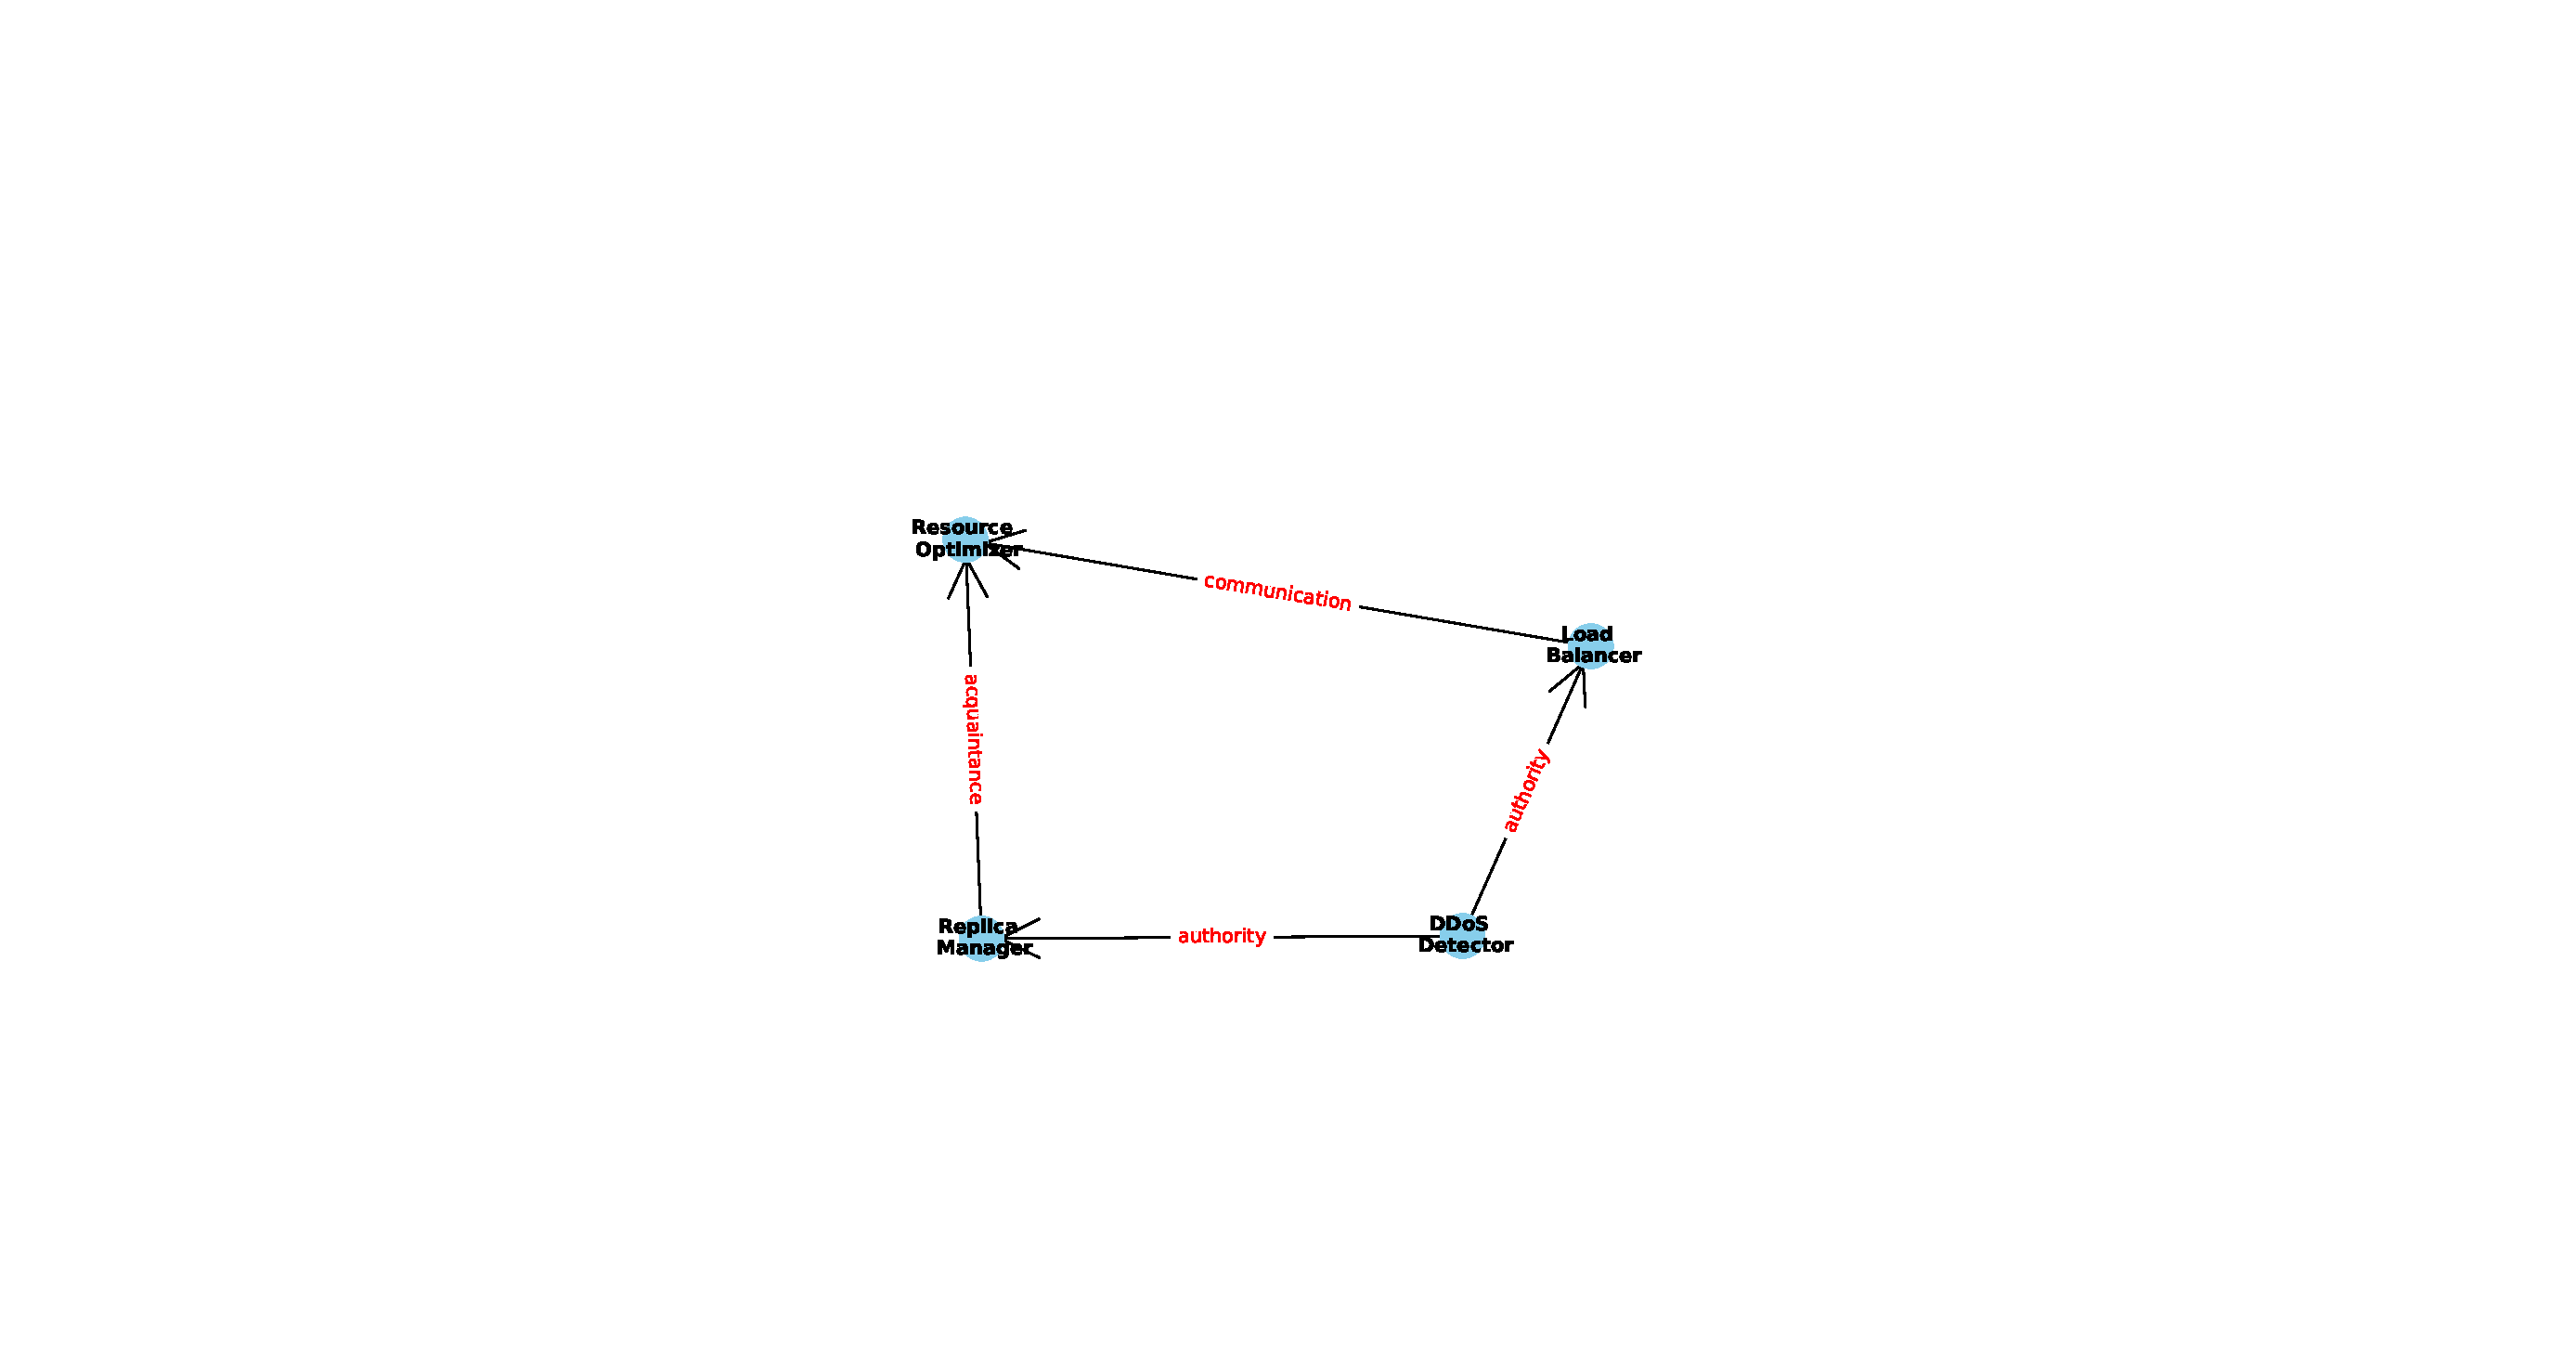
\includegraphics[trim=0cm 2cm 0cm 2cm, clip, width=0.5\textwidth]{figures/roles_graph.pdf}
    \caption{Example of inter-agent graph inferred from trajectories during a DDoS attack: The \textit{DDoS Manager} holds authority over the other agents, coordinating their responses. Additional relations capture observed communication (e.g., Bottleneck and Resource Managers) and awareness links (e.g., acquaintance between Failure and Bottleneck Managers).}
    \label{fig:example_interaction_graph}
\end{figure}

%Considering a time window, we can generate a graph based on detected relations and may evolves dynamically on the next time window, highlighting changes in interaction patterns.

% In addition, we also determine the \textbf{patterns of coordination} that aim to understand the mutual impact of an agent's actions onto another agent's trajectory  over time. Among Sequential Pattern Mining, we favoured the use of the \textit{PrefixSpan} algorithm to identify recurring action sequences across agents during specific scenarios. For example, patterns may show that one agent defers actions to another during adversarial conditions. Detected sequences can be represented as a sequence diagram illustrates how agents interact over time, showing causal relationships and dependencies in resolving challenges.



\subsection{Transfer}
\label{sec:transfer}

% Transfering: Processus de transfert des comportements appris au cluster réel.
%  - récupérer les politiques entrainés dans un sous-module
%  - lancer les politiques entrainés avec l'état courant collecté
%  - appliquer les actions choisies par ces politiques via l'API K8s

In this phase, policies interact with the real cluster:
\begin{enumerate*}[label=\textbf{\arabic*)}, itemjoin={;\quad }]
    \item \textbf{State Collection:} Real-time metrics such as CPU usage, memory consumption, pod status, and network traffic are collected from the Prometheus server~\cite{prometheus}
    \item \textbf{Policy Execution:} Each agent's policy $\pi_i$ computes an action $a_t^i$ based on the current state $s_t$, selecting adjustments such as scaling pod replicas for a deployment
    \item \textbf{Action Application:} The computed actions are sent as API requests, directly modifying deployment.
\end{enumerate*}

Agents in the transfer component continuously interact with the Kubernetes API, generating states that are stored in the modeling component's database. Initially, a large time window is used to collect representative traces for creating a near-realistic digital twin of the Kubernetes cluster. Subsequently, at shorter regular intervals, the modeling component updates the digital twin using the latest trace data. This iterative process aims to ensure agents dynamically adapt to workload.

\noindent \textit{Safety Mechanisms:} To ensure safe policy deployment, KARMA applies several runtime safeguards. Action magnitudes are capped to avoid extreme scaling behaviors, and fallback mechanisms enable reverting to standard KHPA policies if unexpected states are detected. Additionally, policies can be first tested in canary deployments, isolating their effect before full rollout. Monitoring components continuously evaluate agent decisions and trigger alerts if anomalies occur.

%
% The agents interact seamlessly with Kubernetes:
% \begin{enumerate*}[label={}, itemjoin={;\quad }]
%     \item Actions are applied to deployments via the API
%     \item Real-time metrics are gathered using Prometheus, ensuring up-to-date cluster state observations
%     \item KARMA operates independently of the native Kubernetes HPA mechanisms.
% \end{enumerate*}

% \

% \noindent The framework integrates a feedback loop:
% \begin{enumerate*}[label=\textbf{\arabic*)}, itemjoin={;\quad }]
%     \item Metrics from the live cluster are used to update the digital twin model.
%     \item Agents are periodically retrained on this updated model to refine their policies for new workload patterns or adversarial conditions.
%     \item Refined policies are redeployed to the cluster, maintaining high adaptability and resilience.
% \end{enumerate*}

% =======================================
\section{Experimental Setup}
\label{sec:experiments}
% Experimental setup:
%  - Présenter "Chained Services"
%  - CybMASDE: présenter comme un moyen d'implémenter KARMA et présenter la configuration logicielle
%  - Configuration matérielle (pour entrainement et analyse)
%  - Protocole d'experimentation et d'analyse (prend en compte un espèce d'étude d'ablation dans les baselines)
%  - Métriques d'évaluation
%  - Baselines: MA x (Org. Spec.)
%     - modèle sans specifications organisationnelles avec 1 seul agent (état de l'art)
%     - modèle avec spécifications organisationnelles du modèle "fort" avec 1 seul agent (état de l'art?)
%     - modèle sans spécifications organisationnelles avec plusieurs agents (état de l'art?)
%     - modèle avec spécifications organisationnelles du modèle "faible" avec plusieurs agents
%     - modèle avec spécifications organisationnelles du modèle "fort" avec plusieurs agents

This section outlines the experimental setup for evaluating KARMA's ability to address initially defined gaps.

\subsection{Description of the Kubernetes Cluster and Configuration}

The evaluation environment consists of a Kubernetes cluster simulating a \textbf{Chained Services} (CS) architecture. Each service comprises a set of microservices hosted in pods and managed by deployments. For instance, \autoref{fig:chained_services_graph} illustrates the graph representation of a four services CS cluster. We considered using a cluster characterized by the following specifications:

\begin{itemize}
    \item \textbf{Topology:} Four interconnected running services configured to emulate real-world conditions, including resource contention, bottlenecks, and adversarial scenarios;
    \item \textbf{Failure Simulation:} Bottlenecks and cascading failures are induced by resource-intensive workloads, while adversarial conditions (e.g., DDoS attacks) are emulated using Locust~\cite{locust2021} and random-based custom scripts;
    \item \textbf{Worker Nodes:} 1 worker node with 8 vCPUs, 32 GB RAM, and 1 Gbps network bandwidth. This configuration is suitable for testing purposes on medium-sized clusters;
    \item \textbf{Training Node:} 1 high computing cluster comprising nodes with NVIDIA Tesla V100 GPUs (16GB), Intel Xeon Platinum CPUs (2.3 GHz, 16 cores), 128 GB RAM.
\end{itemize}

\begin{figure}[h!]
    \centering
    \hspace{-0.4cm}
    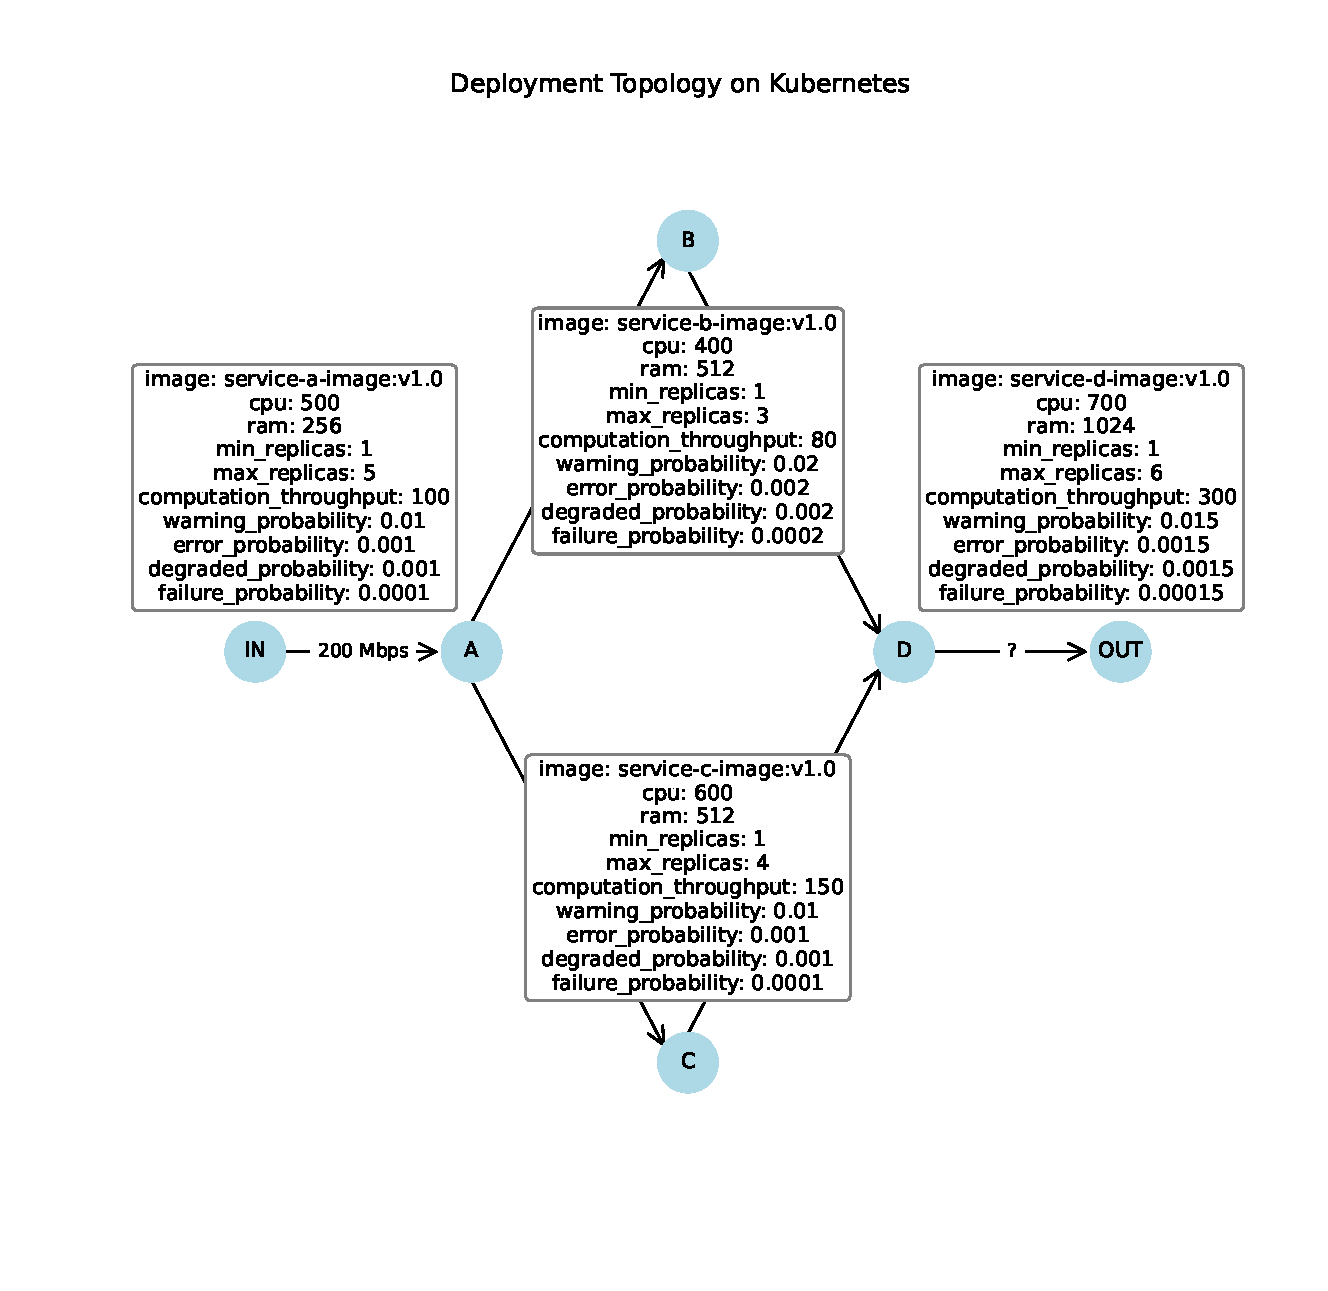
\includegraphics[trim=1.8cm 3.3cm 1.25cm 3.5cm, clip, width=0.5\textwidth]{figures/k8s_cluster_graph.pdf}
    \caption{A graph representation of a "Chained Services" cluster with four services}
    \label{fig:chained_services_graph}
\end{figure}

\subsection{Implementation of KARMA with CybMASDE}

% TODO:
% - Présenter le framework CybMASDE
% - Scénario normal, scénario DDoS (augmentation ponctuelle de volume données), scénario de défaillance (corruption ponctuelle des données), scénario de contention de ressources (priorisation), scénario mixte
% - Protocole d'expérimentation
%   - Baseline 1: Single-Agent w/o Soft Organizational Specifications
%   - Baseline 2: Single-Agent w/ Hard Organizational Specifications
%   - Baseline 3: Multi-Agent w/o Organizational Specifications
%   - Baseline 4: Multi-Agent w/ Organizational Specifications

\footnotetext[2]{\label{lnk:footnote_2}In our implementation by default $\alpha = 3$, $\sigma = 10$, $\kappa = 1$, $ch = 1$, reward weights $(w_1, w_2, w_3, w_4, w_5) = (0.2, 0.2, 0.2, 0.2, 0.2)$, $Q_{\text{threshold}} = 30$ and $U_{\text{threshold}} = 90\%$.
KARMA's source code and other hyperparameters can be found in \url{https://github.com/julien6/KARMA}}

The KARMA framework leverages \textit{Cyber Multi-Agent System Development Environment}~\textsuperscript{\ref{lnk:footnote_2}} (CybMASDE) which is a general assisted-design MAS framework that seamlessly integrates into the KARMA framework.
The framework includes:
\begin{enumerate*}[label=\textbf{\arabic*)}, itemjoin={;\quad }]
    \item \textbf{Digital Twin Modeling:} A simulation environment replicates Kubernetes cluster using real-world traces
    \item \textbf{MARL Training:} \textit{MAPPO}~\cite{Yu2022} is used to train agents in the digital twin environment
    \item \textbf{Organizational Specifications:} Roles and missions defined for agents guide the training process, ensuring coordinated behavior and explainability
    \item \textbf{Deployment Integration:} Trained policies interact with the Kubernetes API to adjust pod replicas in real time.
\end{enumerate*}

\subsection{Roles and Missions for Operational Resilience}

\noindent Following to the $\mathcal{M}OISE^+$~\cite{hubner2002moise} and the AICA architectural insights~\cite{kott2018autonomous}, we implemented four roles to address a specific degradation factor in a QoS.
% and defines the permissible actions of agents.
Each role is associated with a mission, containing a single sub-goal based on metrics.

\noindent \paragraph{\textbf{Bottleneck Manager}} 
%
The \textit{Bottleneck Manager} role is to monitor services for bottlenecks caused by imbalanced traffic flows. It is based on rules following these metrics:
\begin{enumerate*}[label={}, itemjoin={;\quad }]
    \item \( T_{\text{in}}^i \): Incoming traffic for service \( i \) (Kbps)
    \item \( T_{\text{out}}^i \): Outgoing traffic for service \( i \)
    \item \( Q_{\text{pending}}^i \): Pending requests for service \( i \).
\end{enumerate*}
A bottleneck is detected if: $Q_{\text{pending}}^i > Q_{\text{threshold}} \quad \text{or} \quad T_{\text{in}}^i > \alpha \cdot T_{\text{out}}^i$
where \( Q_{\text{threshold}} \) is the critical queue threshold, and \( \alpha > 1 \) is an amplification factor.

The associated mission aims to minimize the pending queue size to eliminate bottlenecks. The reward function is defined as: $R_{\text{bottleneck}} = - \sum_{i} Q_{\text{pending}}^i$
Agents are rewarded for reducing pending requests, optimizing the throughput~\cite{burns2016borg}.

\noindent \paragraph{\textbf{DDoS Manager}}

The \textit{DDoS Manager} role is to identify DDoS attacks by analyzing traffic anomalies:
\begin{enumerate*}[label={}, itemjoin={;\quad }]
    \item \( R_{\text{rate}} \): Incoming request rate for the cluster.
    \item \( L_{\text{avg}} \): Average observed latency.
    \item \( \Delta T \): Change in traffic volume over a time window \( t \).
\end{enumerate*}
A DDoS attack is detected when:
$R_{\text{rate}} > R_{\text{threshold}} \quad \text{and} \quad \Delta T > \Delta T_{\text{threshold}}$
where \( R_{\text{threshold}} \) is a critical traffic threshold.

The associated mission is to isolate affected services to minimize downtime with this reward function:
$R_{\text{ddos}} = - \left( \text{DownTime} \cdot w_{\text{d}} + L_{\text{avg}} \cdot w_{\text{l}} \right)$
where \( w_{\text{d}} \) and \( w_{\text{l}} \) are weights for downtime and latency, respectively~\cite{Liu2018}.

\noindent \paragraph{\textbf{Failure Manager}}

The \textit{Failure Manager} role is to monitor pod health and eliminates failed pods following this rule:
\begin{enumerate*}[label={}, itemjoin={;\quad }]
    \item \( F_{\text{fail}}^i \): Number of failures for pod \( i \)
    \item \( S_{\text{status}}^i \): Status of pod \( i \) (e.g., \textit{CrashLoopBackOff}).
\end{enumerate*}
A pod failure is detected if:
$F_{\text{fail}}^i > F_{\text{threshold}}$
where \( F_{\text{threshold}} \) is the maximum number of tolerated failures.

The associated mission minimizes downtime caused by repeated failures with this reward function:
$R_{\text{failure}} = - \sum_{i} T_{\text{downtime}}^i$
Agents are incentivized to quickly eliminate and restart failed services.

\noindent \paragraph{\textbf{Resource Manager}}

The \textit{Resource Manager} role is to prioritize critical services when resource contention occurs. The rules are based on:
\begin{enumerate*}[label={}, itemjoin={;\quad }]
    \item \( U_{\text{cpu}}^i \): CPU utilization of service \( i \)
    \item \( U_{\text{mem}}^i \): Memory utilization of service \( i \)
    \item \( P_{\text{priority}}^i \): Priority level of service \( i \) (critical, normal, low).
\end{enumerate*}
Contention is detected if total CPU usage exceeds a threshold:
$U_{\text{cpu}}^{\text{total}} > U_{\text{threshold}}$
Non-critical services are scaled down to free resources:
$\text{Replicas}_{\text{new}}^i = \max\left( \text{Replicas}_{\text{current}}^i - \delta, 1 \right)$

The associated mission ensures critical services by balancing resource usage with this reward function:
$R_{\text{resource}} = - \sum_{i \in \text{Critical}} \left( U_{\text{cpu}}^i + U_{\text{mem}}^i \right)$
Agents are rewarded for prioritizing services while maintaining efficient resource usage~\cite{shahrad2020resource}.

\

\subsection{Experimental Protocol}

\noindent To evaluate KARMA's performance in addressing the six gaps, we propose comparing baselines accross scenarios.

\paragraph{\textbf{Real-Cluster Integration \& Evaluation}}

KARMA couples simulation with real-cluster interaction by building a digital twin from real Kubernetes traces. Trained policies are deployed via the Kubernetes API, influencing the real cluster, while new traces refine the simulation. This ensures real-world applicability with agent training in a safe environment.

\paragraph{\textbf{Experimental Scenarios}}

\noindent Five experimental scenarios are defined to simulate key factors impacting operational resilience in Kubernetes:
%
\begin{enumerate*}[label=\textbf{\arabic*)}, itemjoin={;\quad }]
    \item \textbf{Bottleneck Resolution:} Simulates scenarios where upstream services overload downstream services to maximize throughput by dynamically scaling replicas
    \item \textbf{DDoS Attack:} Models a sudden surge in traffic aimed at disrupting critical services to detect the attack, isolate affected services, and minimize downtime~\cite{Liu2018}
    \item \textbf{Pod Failures:} Pod crashes are triggered to evaluate the system's ability to restore affected services~\cite{burns2016borg}
    \item \textbf{Resource Contention:} Simulates high resource demand, requiring dynamic prioritization of critical services to maintain overall cluster functionality~\cite{Vhatkar2022}
    \item \textbf{Mixed Scenario:} Combines all scenarios to evaluate the system's adaptability and resilience.
\end{enumerate*}

\paragraph{\textbf{Baselines from the literature}}
%
\noindent We selected three HPA systems as baselines:
\begin{enumerate*}[label=\textbf{\arabic*)}, itemjoin={;\quad }]
    \item \textbf{AWARE:} An RL-based system that balances response time and throughput~\cite{aware2023}
    \item \textbf{Gym-HPA:} An RL environment for experimentation with various RL algorithms in simulation~\cite{gymhpa2022}
    \item \textbf{Rlad-core}~\cite{Rossi2019} A RL-based simulator which uses machine learning techniques to scale services, most notably Q-learning and Model-based algorithms.
\end{enumerate*}

These baselines have been tested under the same five scenarios using source code when available.

\paragraph{\textbf{Baselines as ablation studies}}

\noindent To isolate the contributions of KARMA's components, ablation studies have been performed following these configurations:
%
\begin{itemize}
    \item \textbf{With/without MLP:} Evaluates the impact of using an MLP-based transitioner for digital-twin modeling.
    \item \textbf{With/without organizational specifications:} Tests hard and soft organizational constraints during training:
        \begin{itemize}
            \item \textit{Hard constraints:} Strictly enforce roles and missions.
            \item \textit{Soft constraints:} Allow exploratory actions with rewards based on organizational specifications.
        \end{itemize}
    \item \textbf{Multi-agent vs Mono-agent:} Compares a multi-agent configuration with a mono-agent baseline.
\end{itemize}

\paragraph{\textbf{Performance Metrics}}

\noindent For each scenario and baseline, the following metrics are collected:
%
\begin{enumerate*}[label=\textbf{\arabic*)}, itemjoin={;\quad }]
    \item \textbf{Operational Resilience:} Based on the global reward from the success rate (\%), ratio of pending request (\%), average latency (ms)
    \item \textbf{Adversarial Robustness:} Based on the standard deviation of the reward and the recovery time after DDoS (s), percentage of services remaining available (\%)
    \item \textbf{Digital Twin Accuracy:} Based on the modeled transition model accuracy (\%), computed as the ratio of real cluster performance over the simulation's one
    \item \textbf{Automated MAS Generation:} Based on training convergence time (number of episodes)
    \item \textbf{Adaptability:} Based on the reward standard deviation variance over training episodes on all scenarios (\%)
    \item \textbf{Explainability:} Based on alignment of behaviors with roles/missions when given (\%), and qualitative evaluation of clustering of trajectories.
\end{enumerate*}



\section{Results and Discussion}
\label{sec:results}

This section analyzes the performance of KARMA in addressing the six identified gaps.


\subsection{Gap 1: Operational Resilience}
Operational resilience evaluates the ability of the system to handle failures and maintain high QoS.
\begin{table}[h]
    \centering
    \caption{Operational resilience metrics across all scenarios.}
    \label{tab:operational_resilience}{\footnotesize
    \begin{tabular}{>{\raggedright\arraybackslash}m{2.7cm}>{\centering\arraybackslash}m{1.5cm}>{\centering\arraybackslash}m{1.5cm}>{\centering\arraybackslash}m{1.5cm}}
        \hline
        \textbf{Baseline} & \textbf{Success Rate (\%)} & \textbf{Latency Compliance (\%)} & \textbf{Pending Requests (\%)} \\
        \hline
        KHPA & 64.8 & 58.1 & 20.7 \\
        Gym-HPA & 73.1 & 65.7 & 20.8 \\
        Rlad-core & 77.4 & 70.1 & 15.9 \\
        AWARE & 80.6 & 73.8 & 13.3 \\
        Single-Agent w/o Org. Spec. & 72.6 & 65.4 & 17.0 \\
        Single-Agent w/ Hard Org. Spec. & 80.8 & 72.5 & 15.4 \\
        Multi-Agent w/o Org. Spec. & 87.7 & 81.5 & 9.3 \\
        Multi-Agent w/ Soft Org. Spec. & 82.0 & 74.7 & 15.0 \\
        \textbf{Multi-Agent w/ Hard Org. Spec. (KARMA)} & \textbf{90.9} & \textbf{85.7} & \textbf{5.9} \\
        \hline
    \end{tabular}}
\end{table}
%
\autoref{tab:operational_resilience} presents a comparison of KARMA against existing baselines. The results show that KARMA achieves the highest success rate (\textbf{90.9\%}), surpassing all baselines including AWARE (80.6\%) and Rlad-core (\textbf{77.4\%}). Similarly, the latency compliance of KARMA is the highest at \textbf{85.7\%}, while the lowest pending requests ratio (\textbf{5.9\%}) suggests efficient handling of workload variations.

\noindent \textit{Statistical Note:} All reported values represent the mean over 10 independent evaluation runs. Although not shown in the tables for brevity, the standard deviation across runs remained consistently low ($\pm$1.8\% for success rate and $\pm$2.1 ms for latency in the mixed scenario), indicating robust outcomes.

KARMA's performance stems from its structured multi-agent coordination, which optimally distributes resources based on failure contexts, avoiding redundant or conflicting scaling actions—issues common in single-agent RL-based autoscalers.
%
Reactive, threshold-based autoscalers like KHPA and Gym-HPA struggle with dynamic workloads, leading to higher pending requests and lower success rates. AWARE and Rlad-core improve response time and throughput but lack multi-agent coordination, resulting in slower reactions in adversarial scenarios. Single-Agent w/o Organizational Specifications suffers from inefficient resource allocation, while Single-Agent w/ Hard Organizational Specifications benefits from structured decision-making but still lacks distributed coordination.

KARMA's role-based coordination minimizes inefficiencies and enhances decision stability. Its hierarchical decomposition of objectives enables independent yet complementary decisions, leading to more resilient autoscaling.

The results also underscore the value of organizational constraints. Multi-agent systems with soft constraints (82.0\% success rate) outperform single-agent approaches, but KARMA's hard constraints achieve the best results, eliminating conflicting agent behaviors and optimizing scaling.



\subsection{Gap 2: Adversarial Conditions}

Adversarial conditions evaluate the system's robustness against disruptive scenarios such as DDoS attacks.
\begin{table}[h]
    \centering
    \caption{Performance under DDoS scenario.}
    \label{tab:adversarial_conditions}{
        \footnotesize
    \begin{tabular}{>{\raggedright\arraybackslash}m{3.6cm}>{\centering\arraybackslash}m{1.8cm}>{\centering\arraybackslash}m{2cm}}
        \hline
        \textbf{Baseline} & \textbf{Recovery Time (s)} & \textbf{Service Availability (\%)} \\
        \hline
        KHPA & 80.7 & 65.6 \\
        Gym-HPA & 66.2 & 72.6 \\
        Rlad-core & 37.4 & 78.3 \\
        AWARE & 49.5 & 83.6 \\
        Single-Agent w/o Org. Spec. & 60.3 & 72.4 \\
        Single-Agent w/ Hard Org. Spec. & 48.5 & 77.5 \\
        Multi-Agent w/o Org. Spec. & 43.5 & 82.0 \\
        Multi-Agent w/ Soft Org. Spec. & 38.8 & 86.0 \\
        \textbf{Multi-Agent w/ Hard Org. Spec. (KARMA)} & \textbf{33.0} & \textbf{90.7} \\
        \hline
    \end{tabular}}
\end{table}
%
\autoref{tab:adversarial_conditions} compares recovery times and service availability in the \textit{DDoS Attack} scenario. KARMA achieves the fastest recovery time (\textbf{33.0s}), outperforming AWARE (\textbf{38.8s}) and Rlad-core (\textbf{43.5s}). It also ensures a good service availability at \textbf{90.7\%}, reducing downtime compared to AWARE (\textbf{83.6\%}).

Traditional autoscalers like KHPA and Gym-HPA rely on reactive threshold-based scaling, leading to slower recovery and lower service availability under attacks. RL-based methods such as Rlad-core and AWARE improve resilience but lack structured coordination, making them less effective against adversarial spikes. Single-agent approaches struggle with balancing attack mitigation and resource optimization, while multi-agent models with soft constraints allow exploratory actions that sometimes delay optimal responses.

KARMA's proactive adversarial learning and structured coordination enable it to anticipate attacks rather than react after degradation. Explicit role-based constraints ensure agents prioritize critical scaling actions, resulting in faster mitigation and higher availability. These results highlight the effectiveness of multi-agent structured learning in security-sensitive autoscaling, where traditional methods exhibit slower adaptation and prolonged downtime.


\subsection{Gap 3: Digital Twin Modeling}

\begin{table}[h]
    \centering
    \caption{Transition models accuracy across all scenarios.}
    \label{tab:digital_twin_accuracy}{
        \footnotesize
    \begin{tabular}{>{\raggedright\arraybackslash}m{6cm}>{\centering\arraybackslash}m{2cm}}
        \hline
        \textbf{Baseline} & \textbf{Accuracy (\%)} \\
        \hline
        Without MLP Transition Model & 83.5 \\
        \textbf{With MLP Transition Model (KARMA)} & \textbf{94.9} \\
        \hline
    \end{tabular}}
\end{table}
%
The accuracy of the digital twin model is critical for training agents under realistic conditions.
\autoref{tab:digital_twin_accuracy} compares the accuracy of different digital twin models. The results show that KARMA achieves \textbf{94.9\%} accuracy, outperforming the non-MLP model (\textbf{83.5\%}), which struggles to generalize.

The improvement stems from the MLP model's ability to capture non-linear dependencies between workload fluctuations, resource allocation, and scaling actions. Without this feature, the system fails to model complex cluster behaviors accurately.
%
By leveraging a neural network for transition modeling, KARMA ensures a more reliable digital twin, allowing agents to train under near-realistic conditions. This reduces the risk of poor decision-making when policies transfer to production, reinforcing the importance of high-fidelity simulations.



\subsection{Gap 4: Automated MAS Generation}

The efficiency of generating a MAS is evaluated in terms of convergence time and training overhead. \autoref{tab:mas_generation_efficiency} presents the results across concerned scenarios while \autoref{fig:learning_curves} shows learning curves in the mixed scenario over 2000 episodes.

\begin{table}[h]
    \centering
    \caption{MAS generation efficiency across all scenarios.}
    \label{tab:mas_generation_efficiency}{
        \footnotesize
    \begin{tabular}{>{\raggedright\arraybackslash}m{3.5cm}>{\centering\arraybackslash}m{2cm}>{\centering\arraybackslash}m{2cm}}
        \hline
        \textbf{Baseline} & \textbf{Convergence Time (episodes)} & \textbf{Training Overhead (hours)} \\
        \hline
        Multi-Agent w/o Org. Spec. & 1800 & 4 \\
        \textbf{Multi-Agent w/ Hard Org. Spec. (KARMA)} & \textbf{950} & \textbf{1.5} \\
        \hline
    \end{tabular}}
\end{table}

The role-guided learning narrows the search space for optimal policies, enabling faster convergence and reduced computational costs. These efficiency gains are particularly important for scaling MAS solutions to complex environments.

The learning curves in \autoref{fig:learning_curves} demonstrate that KARMA achieves stable convergence significantly faster than the baseline without organizational specifications. By episode 950, KARMA exhibits minimal variance in cumulative rewards, whereas the baseline requires nearly double the episodes (1800) to reach comparable performance. This highlights the role of organizational constraints in guiding agents toward effective policies, thereby reducing exploration overhead.

\noindent \textit{Overhead Discussion:} The training phase for KARMA required approximately 1.5 hours on a high-performance machine with 1 GPU (Tesla V100, 16GB) and 16 CPU cores, converging in under 1,000 episodes. At inference time, each agent's policy produces decisions in under 30ms, with a negligible memory footprint (<50MB per agent).

\autoref{tab:mas_generation_efficiency}, shows reduced \textit{Convergence Time} by approximately \textbf{47\%} compared to Multi-Agent w/o Org. Spec., showcasing the efficiency of role-guided learning in minimizing unnecessary exploration. Moreover, \textit{Training Overhead} is reduced by \textbf{62.5\%}, showing a better practicality for large-scale systems where computational resources are a limiting factor.

\begin{figure}[h!]
    \centering
    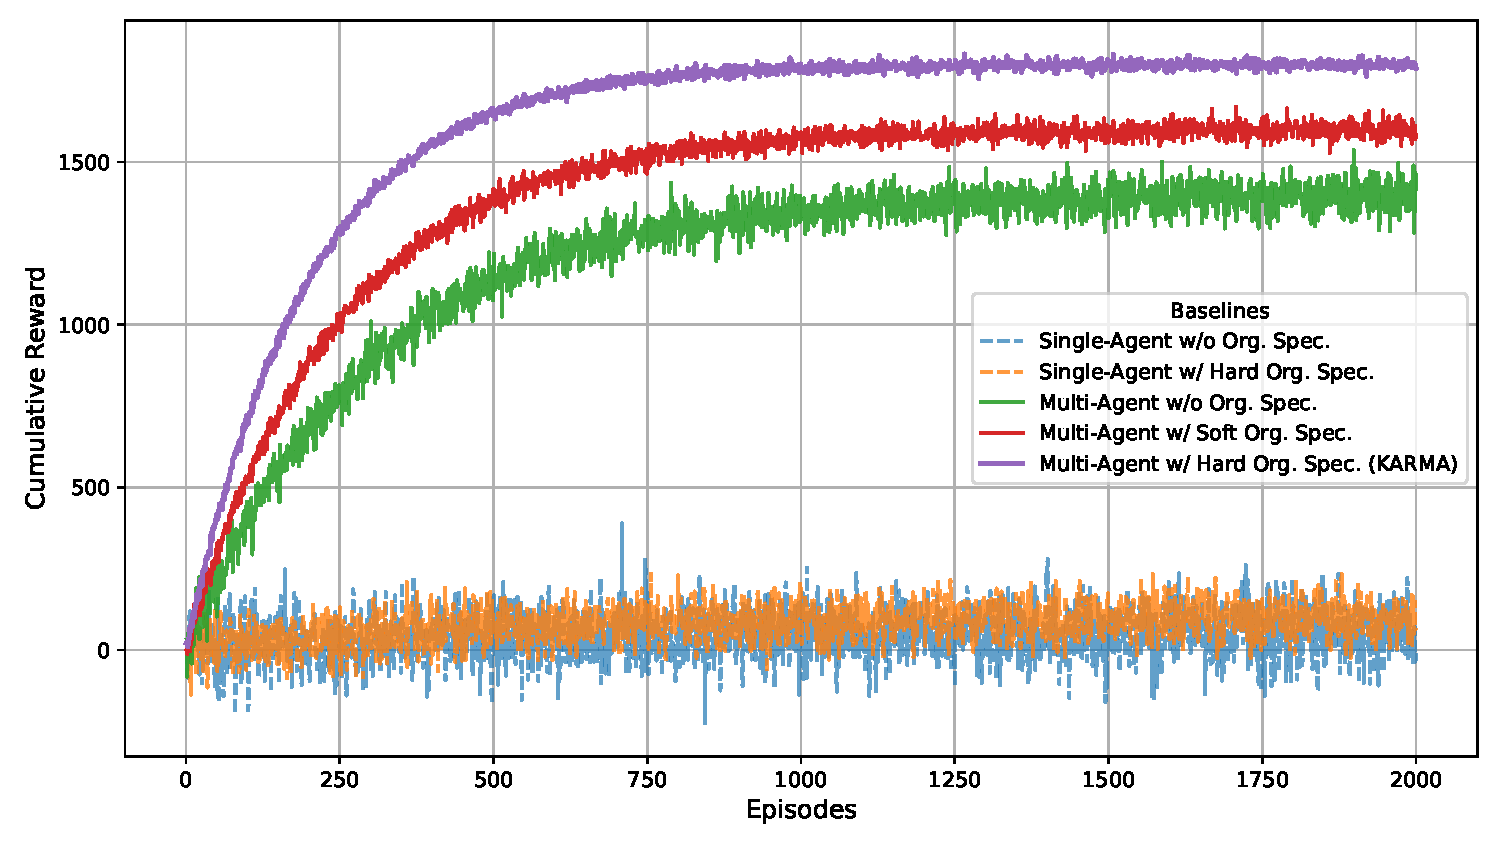
\includegraphics[width=0.49\textwidth]{figures/learning_curves.pdf}
    \caption{Learning curves across baselines for the mixed scenario over 2000 episodes.}
    \label{fig:learning_curves}
\end{figure}


\subsection{Gap 5: Adaptability}

Adaptability assesses the ability of the system to maintain performance under dynamic workloads accross scenarios.
\begin{table}[h]
    \centering
    \caption{Comparison of adaptability in the mixed scenario.}
    \label{tab:adaptability_comparison}{
    \footnotesize
    \begin{tabular}{>{\raggedright\arraybackslash}m{5cm}>{\centering\arraybackslash}m{3cm}}
        \hline
        \textbf{Baseline} & \textbf{Reward s.t.d (\%)} \\
        \hline
        Single-Agent w/o Org. Spec. & 11.1 \\
        Single-Agent w/ Hard Org. Spec. & 11.1 \\
        Multi-Agent w/o Org. Spec. & 10.7 \\
        Multi-Agent w/ Soft Org. Spec. & 9.0 \\
        \textbf{Multi-Agent w/ Hard Org. Spec. (KARMA)} & \textbf{5.3} \\
        \hline
    \end{tabular}}
\end{table}
%
\autoref{tab:adaptability_comparison} shows that KARMA achieves the lowest reward standard deviation (\textbf{5.3\%}), indicating a highly stable performance, outperforming Multi-Agent w/ Soft Org. Spec. (\textbf{9.0\%}) and Multi-Agent w/o Org. Spec. (\textbf{10.7\%}).

In the \textit{Mixed Scenario}, single-agent models exhibit higher variance as they must balance multiple competing objectives without specialization. Multi-agent approaches improve adaptability, but without structured coordination, fluctuations remain. The use of soft organizational constraints stabilizes performance, though some exploratory variations persist.

KARMA's hierarchical reinforcement learning ensures lower variability by decomposing the overarching goal into specialized sub-goals. This structured approach enables agents to focus on well-defined objectives, reducing conflicting decisions and improving overall stability.
%
These findings underscore the importance of structured learning frameworks in autoscaling. By enforcing clear agent specializations, KARMA enhances adaptability, ensuring resilient performance across unpredictable workload conditions.


\subsection{Gap 6: Explainability}
\label{subsec:gap_explainability}

Explainability is qualitatively evaluated through trajectory clustering and quantitatively through the alignment of agent behaviors with predefined roles and missions.
\noindent \autoref{fig:trajectory_clustering_hrl} illustrates the dendrogram generated by hierarchical clustering of agents' action sequences with the four roles applied, using DTW as the similarity measure. The figure highlights the emergence of four distinct clusters, each corresponding to a specific organizational role, demonstrating the ability of the agents' behaviors to align with the predefined roles.

\begin{figure}[h!]
    \centering
    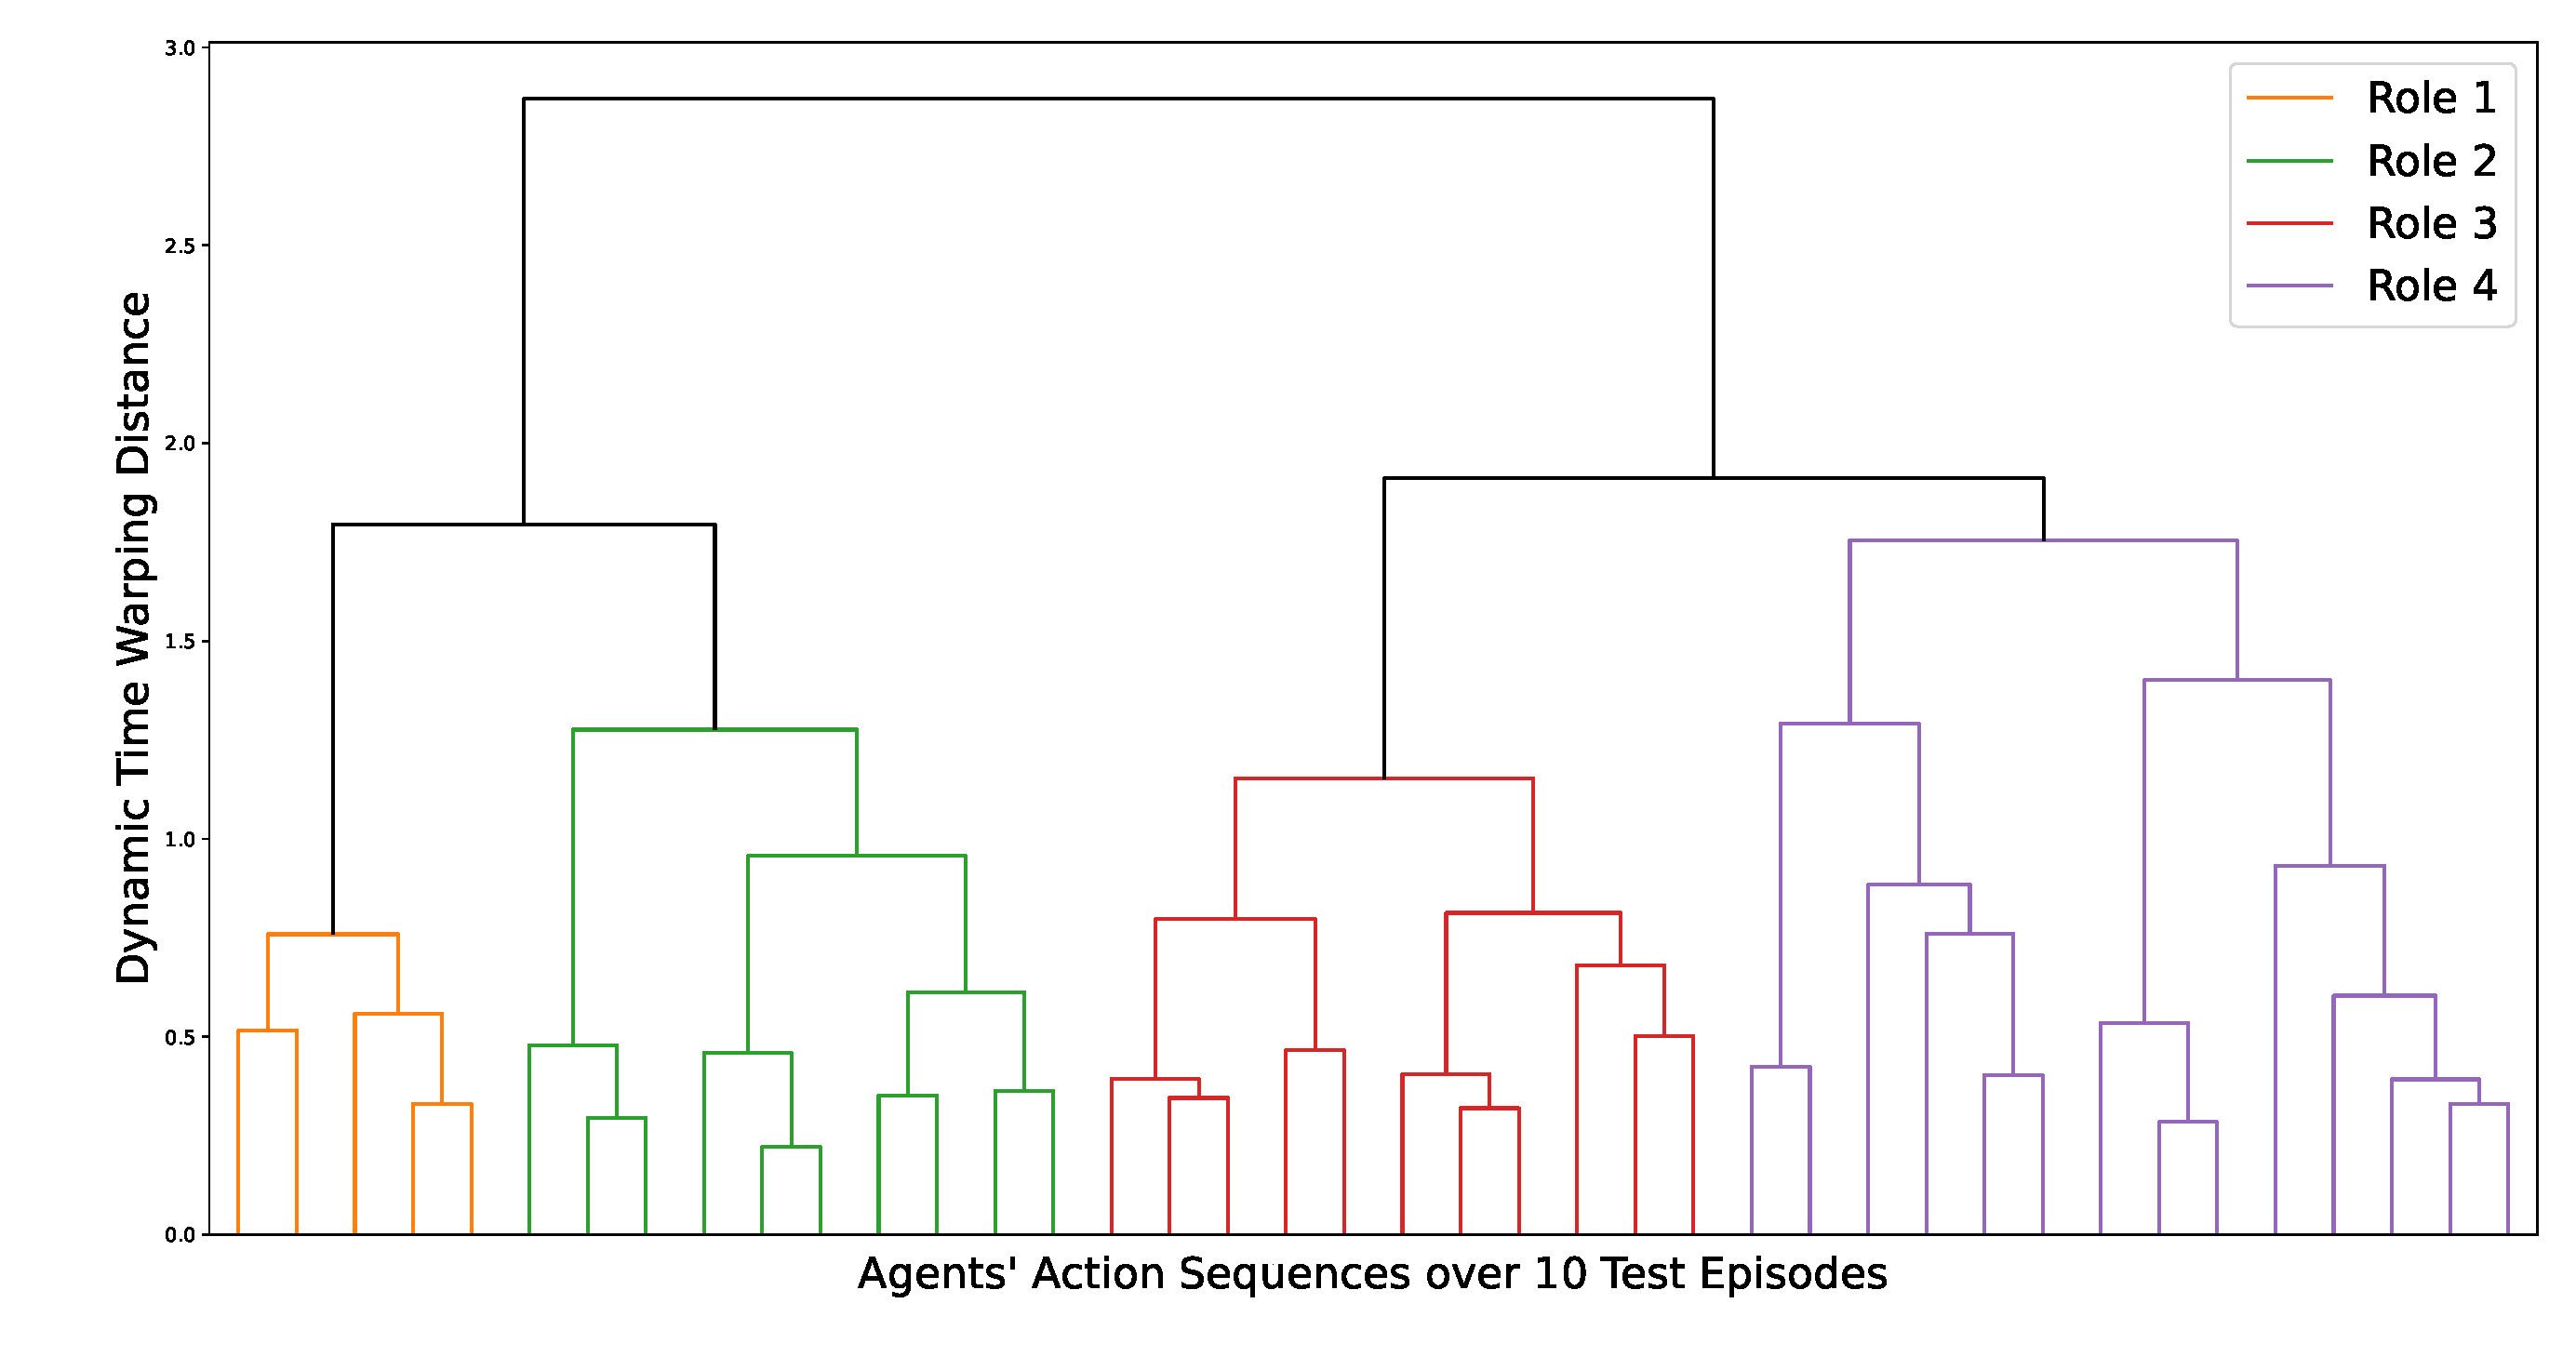
\includegraphics[width=0.49\textwidth]{figures/role_hierarchical_clustering.pdf}
    \caption{Dendrogram obtained after hierarchical clustering of agent trajectories for role inference in the mixed scenario.}
    \label{fig:trajectory_clustering_hrl}
\end{figure}

\begin{table}[h!]
    \centering
    \caption{Alignment of agents with roles and missions.}
    \label{tab:alignment}
    {\footnotesize
    \begin{tabular}{>{\raggedright\arraybackslash}m{4.1cm}>{\centering\arraybackslash}m{1.5cm}>
    {\centering\arraybackslash}m{1.5cm}}
    \toprule
    \textbf{Baseline} & \textbf{Alignment Score (\%)} & \textbf{Clustering Purity (\%)} \\
    \midrule
    Multi-Agent w/o Org. Spec. & $\emptyset$ & 62.7 \\
    Multi-Agent w/ Soft Org. Spec. & 85.3 & 70.1 \\
    \textbf{Multi-Agent w/ Hard Org. Spec. (KARMA)} & \textbf{96.2} & \textbf{89.4} \\
    \bottomrule
    \end{tabular}
    }
\end{table}

KARMA shows the emergence of distinct behavioral patterns aligned with predefined roles validates KARMA's organizational model and has the highest alignment score (\textbf{96.2\%}), significantly outperforming Multi-Agent w/o Org. Spec. (\textbf{85.3\%}), showcasing well-coordinated agent behaviors. In adversarial scenarios, clustering purity is highest for KARMA, reflecting the clear differentiation of agent behaviors under organizational constraints.
%
Distinct clusters validate the role-specific behaviors and highlight the interpretability of agents. Baselines without organizational specifications show reduced explainability, as evidenced by lower clustering purity and alignment scores with soft organizational constraints.

\subsection{General discussion}

The experimental results demonstrate that KARMA effectively addresses several critical gaps in Kubernetes autoscaling. By integrating MARL with organizational principles, KARMA achieves notable improvements in operational resilience, adversarial robustness, and explainability. Its ability to decompose complex goals into roles and missions ensures coordinated agent behavior, as reflected in the high success rates, reduced recovery times, and alignment with predefined roles observed across all scenarios. The use of a digital twin environment, enhanced by an MLP-based transition model, further strengthens KARMA's capacity to simulate realistic conditions, facilitating robust training and better policy generalization.

However, KARMA is not without limitations. While it shows advancements in adaptability, its dependence on domain expertise for defining roles and missions could limit its applicability in domains where such expertise is scarce. Additionally, the computational overhead required for multi-agent training and digital twin modeling remains a challenge for large-scale deployments. The results also indicate that while KARMA effectively reduces latency and pending requests, some baselines, such as Rlad-core, perform comparably in specific scenarios like resource contention, highlighting areas where further refinement may be needed.

\section{Conclusion}
\label{sec:conclusion}
% Conclusion
%  - Résumé
%  - Résumé des Points faibles et Perspectives

This paper presented KARMA, a framework aimed at improving the operational resilience of Kubernetes clusters. While modular designs offer simplicity, they often rely on manual coordination that struggles in dynamic or adversarial contexts. In contrast, KARMA’s MAS approach enables adaptive, decentralized responses through agent specialization.
The experimental results demonstrate that KARMA effectively addresses several critical gaps in Kubernetes autoscaling. By integrating MARL with organizational principles, KARMA achieves improvements in adversarial robustness, and explainability. Its ability to decompose complex goals into roles and missions ensures coordinated agent behavior. The use of MLP-based transition model, further strengthens KARMA's capacity to simulate realistic conditions.
%
% The main contributions of this work include:
% \begin{itemize}
%     \item \textbf{Digital Twin Environment:} A realistic and representative simulation model derived from cluster traces, enabling safe and efficient policy learning through a digital twin.
%     \item \textbf{Organizationally Guided Design:} The use of roles and missions to decompose operational resilience into manageable sub-goals, providing a systematic method for agent coordination and decision-making.
%     \item \textbf{Multi-Agent Reinforcement Learning (MARL):} Leveraging MARL algorithms to train agents collaboratively, ensuring adaptability and robustness in complex, multi-goal scenarios.
%     \item \textbf{Explainability and Analysis:} Analyzing agent behaviors using trajectory clustering and inter-agent interaction detection, enhancing interpretability and trust in agent decisions.
%     \item \textbf{Adversarial Scenario Handling:} Demonstrating the resilience of the proposed framework in scenarios such as DDoS attacks, which are critical for the reliability of cloud-native systems.
% \end{itemize}
%
% \

However, some aspects need to be further explored:
\begin{enumerate*}[label=\textbf{\arabic*)}, itemjoin={;\quad }]
    \item \textbf{Simulation-to-Reality Gap:} Even though we generate a near-realistic simulation model from environment traces, we need to better simulate unaccounted unexpected system failures
    \item \textbf{Dependence on Domain Expertise:} Defining roles, missions, and reward structures relies heavily on domain-specific knowledge, which may limit the framework's generalizability
    \item \textbf{Computational Overhead:} The training process with multi-agent configurations and organizational constraints requires substantial computational resources.
    \item \textbf{Scalability to Multi-Node Clusters:} Although current experiments focus on a single-node cluster, preliminary evaluations are being conducted on larger-scale deployments.

    % \item \textbf{Sensitivity to Workload Shifts:} While KARMA demonstrates adaptability, abrupt changes in workload patterns or cluster configurations may require retraining or fine-tuning of agent policies.
    % \item \textbf{Evaluation Scope:} Although the framework was tested under diverse scenarios, including adversarial conditions, its performance on larger and more heterogeneous clusters remains to be validated.
\end{enumerate*}


% While KARMA is not a universal solution to all Kubernetes autoscaling challenges, it provides a step forward in addressing key gaps in operational resilience, adaptability, and explainability. The framework's combination of MARL and organizational principles offers a promising foundation for future research and development.


\chapter{Résultats expérimentaux et analyse comparative}
\section{Validation expérimentale des hypothèses}
\section{Comparaison entre scénarios}
\section{Discussion des résultats et généralité}

\chapter*{Conclusion}
\addcontentsline{toc}{chapter}{\textbf{Conclusion}}
% TODO
